\documentclass{article}
\usepackage{graphicx} % Required for inserting images
\usepackage[utf8]{inputenc} % UTF-8 kódolás
\usepackage[T1]{fontenc} % Magyar ékezetek
\usepackage{hyphenat} % Kötőjelezés támogatása
\usepackage[top=2cm, bottom=2cm, left=2cm, right=2cm]{geometry} % Margók beállítása
\usepackage{float} % Képek abszolút elhelyezése

\title{\textbf{Magas rendelkezésreállású beágyazott rendszerek}}
\author{Diasor: Prof. Dr. Molnár András, Jegyzet: py-snake}
\date{2025. november}

\begin{document}

\maketitle

\section{Követelmények}

\begin{itemize}
    \item 1 db zh
    \item évközi jegy
    \item élév végén zh
    \item pótlás: csak annak, aki nem írta meg
\end{itemize}

\section{Bevezetés}

\begin{figure}[H]
    \centering
    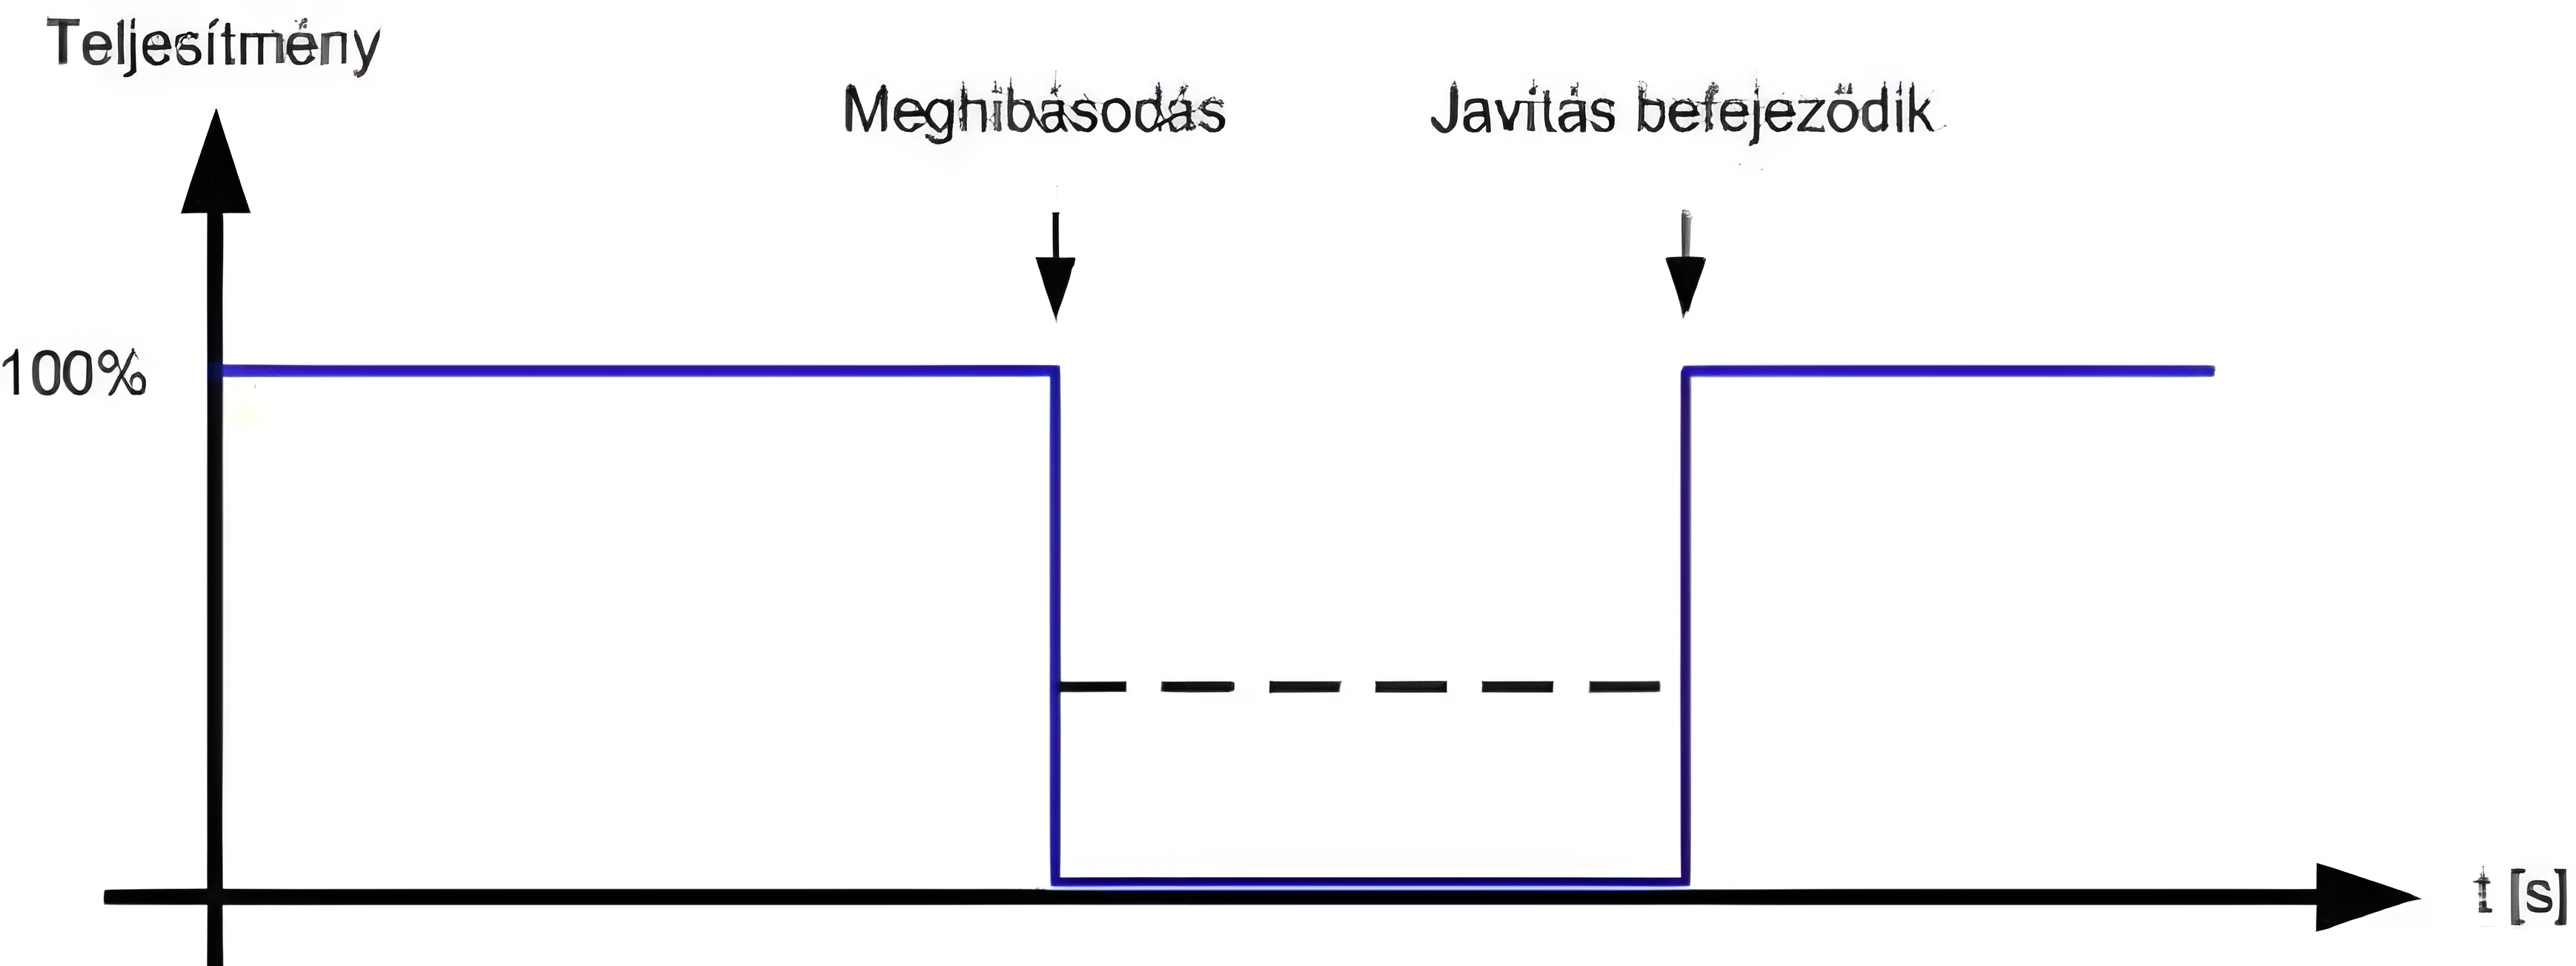
\includegraphics[width=0.7\textwidth]{kep/kep1.png}
    \caption{Egy rendszer rendelkezésreállása}
    \label{fig:kep1}
\end{figure}

\begin{itemize}
    \item \textbf{Beágyazott rendszerek}
    \item \textbf{Redundáns rendszerek}
\end{itemize}

\begin{itemize}
    \item Olyan rendszerek, amelyek nagyon nagy megbízhatósággal képesek üzemelni.
    \item \textbf{Hiba esetén egy rendszer nem állhat le teljesen;} legrosszabb esetben is minimum korlátozott módon kell üzemelnie, amíg meg nem történik a javítás.
    \item \textbf{Redundáns:} a rendszer összetevői többszörözve vannak a megbízhatóság érdekében.
    \item \textbf{Hiba detektálása:} nem biztos, hogy észrevesszük, ha valami elromlik.
    \item \textbf{A hiba feltárása problémás lehet,} még ha tudjuk is, hogy valamilyen hiba van ki kell deríteni, melyik komponens jelez hibát, és minek a meghibásodása okozta a jelenséget.
\end{itemize}

\section{A hibajelenség okát ki kell deríteni}

\begin{itemize}
    \item Mi a konkrét hiba?
    \item Mi a forrás?
    \item Szoftveres vagy hardveres hiba?
    \item Szoftverhiba: nem volt felkészítve a kód bizonyos esetekre, nem tudja kezelni a beérkező értékeket, és ez gondot okoz.
    \item Hardver hiba: megsérült egy adott szenzor.
\end{itemize}

\section{A hibák lehetséges forrásai}

\begin{figure}[H]
    \centering
    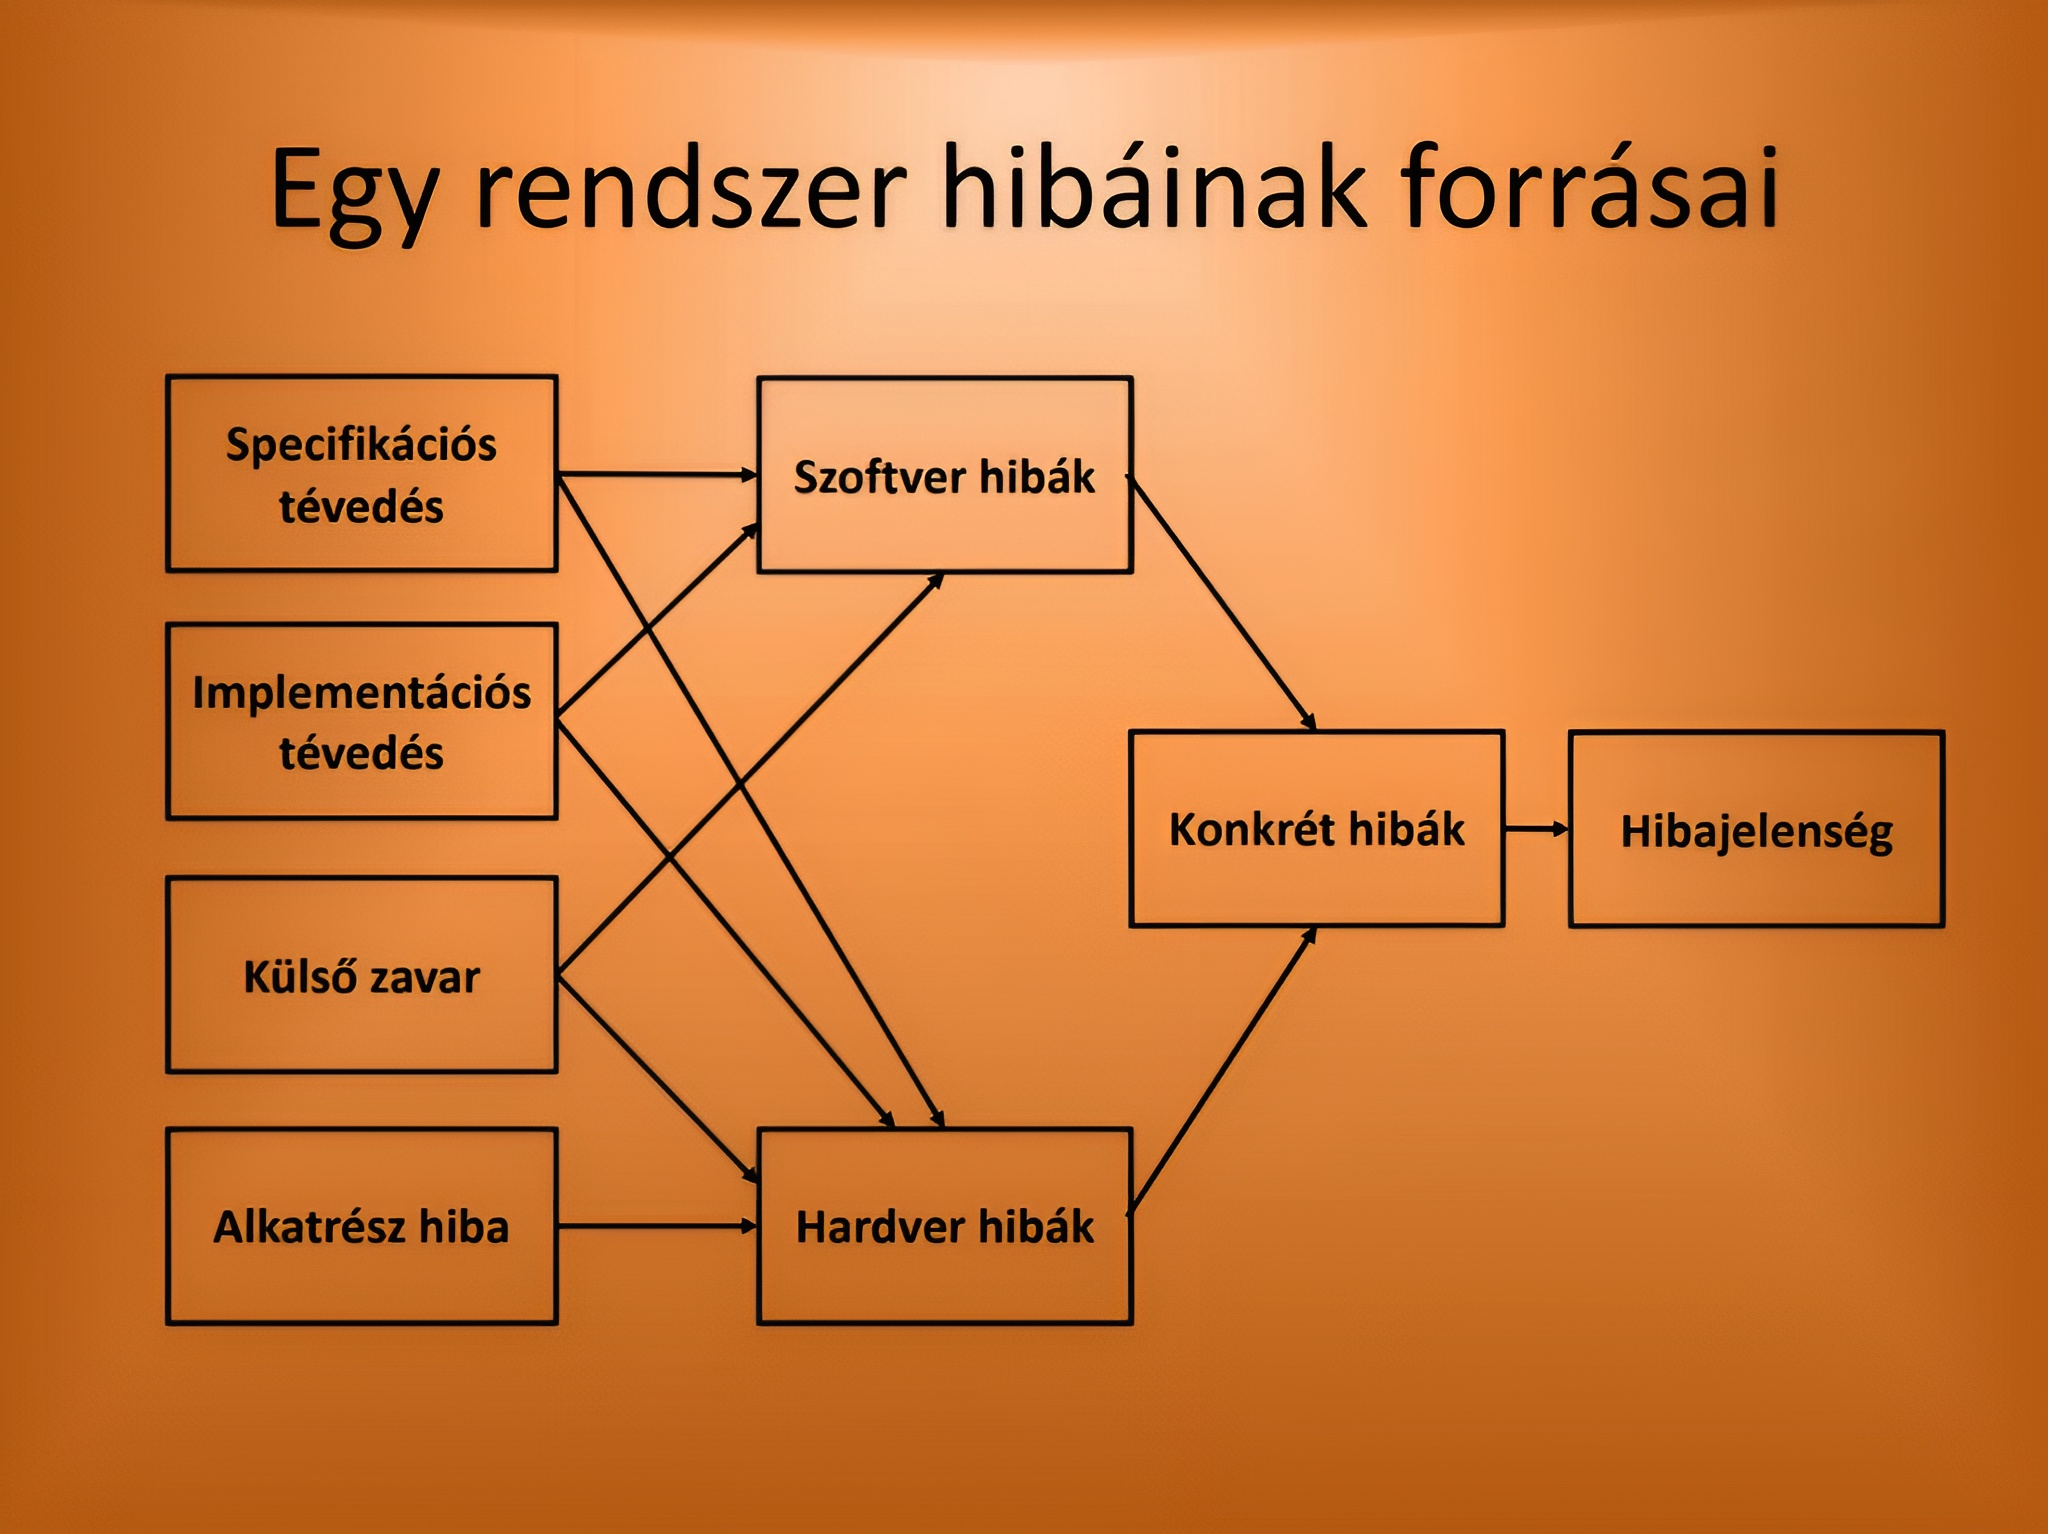
\includegraphics[width=0.7\textwidth]{kep/kep2.png}
    \caption{Egy rendszer hibáinak forrásai}
    \label{fig:kep2}
\end{figure}

\begin{itemize}
    \item \textbf{Specifikációs tévedés:} már a tervben hiba van, és a hibás elv alapján lett elkészítve a szoftver vagy a hardver. Pl: alulméretezett tengely, vagy a kód a specifikációnak megfelel, de a valóságnak nem.
    \item \textbf{Implementációs tévedés:} Például a tengely rossz méretezéssel lett elkészítve, ugyan működik de meg fog hibásodni a rossz kivitelezés miatt. Vagy pl: rosszul lett elkészítve a kód, például 0-val való osztásra fut.
    \item \textbf{Külső zavar:} kívülről érkező tényező zavart okoz a hardverben vagy szoftverben. Például valamilyen sugárzás éri a hardvert, vagy kibertámadás a szoftvert.
    \item \textbf{Alkatrész hiba:} valamilyen alkatrész idő előtt tönkremegy egy áramkörben, de ez is korrigálható, ha úgy van tervezve az eszköz, hogy valami más átvegye a szerepét.
\end{itemize}

\begin{figure}[H]
    \centering
    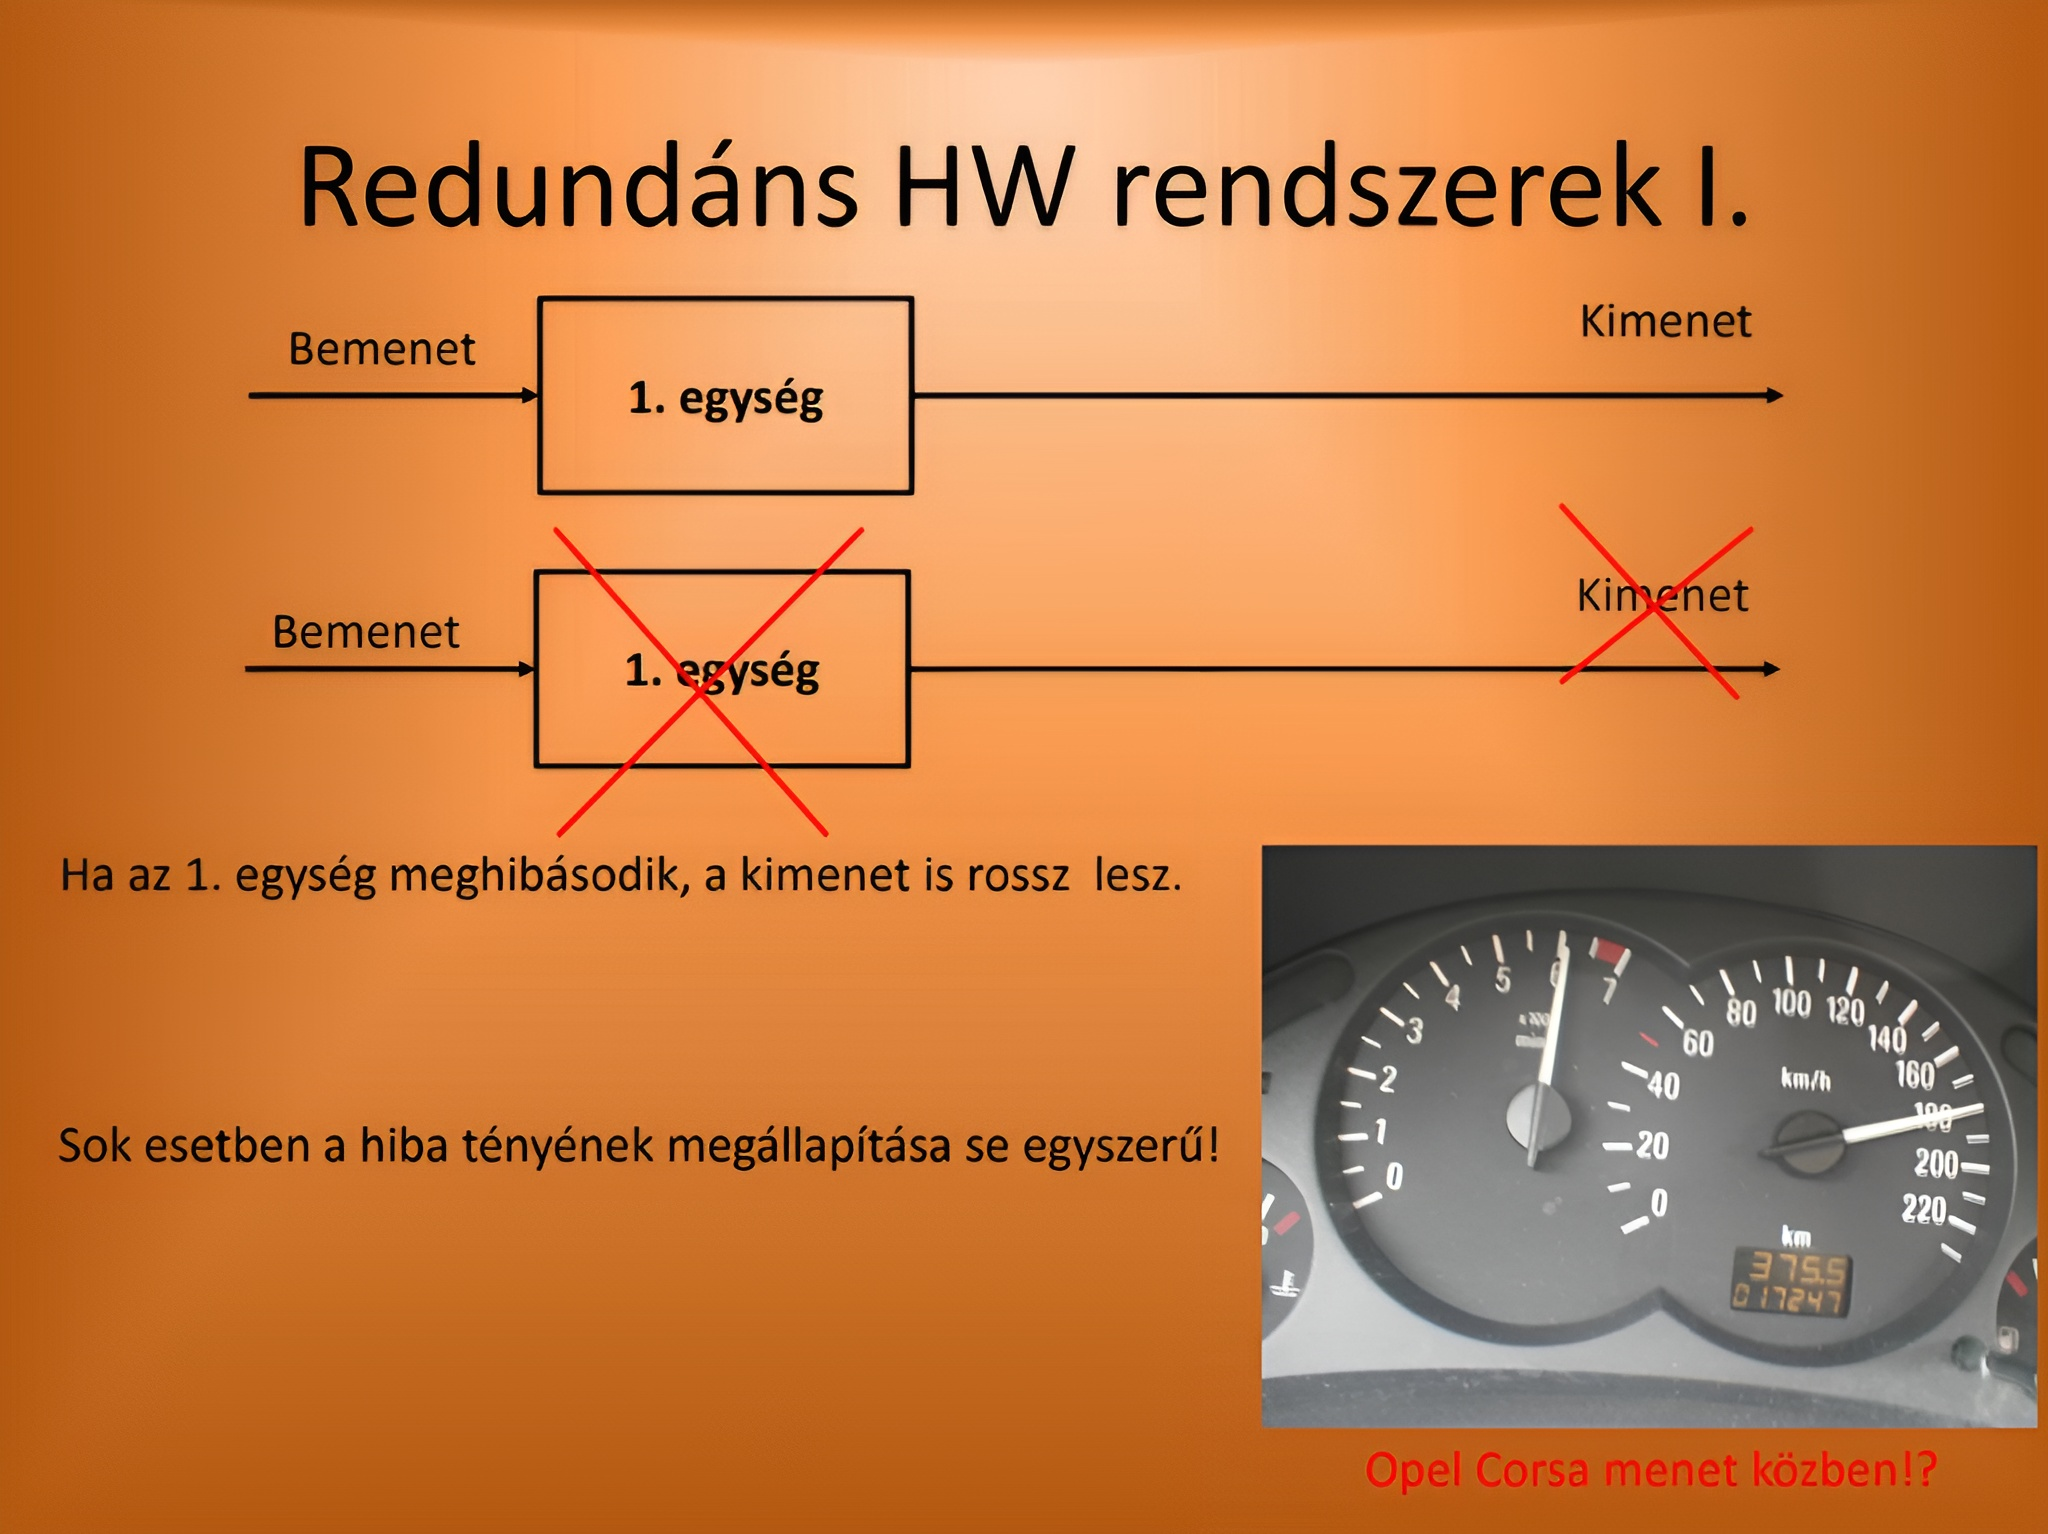
\includegraphics[width=0.7\textwidth]{kep/kep3.png}
    \caption{Redundáns HW rendszerek I. - 1 egységből álló rendszer}
    \label{fig:kep3}
\end{figure}

\begin{figure}[H]
    \centering
    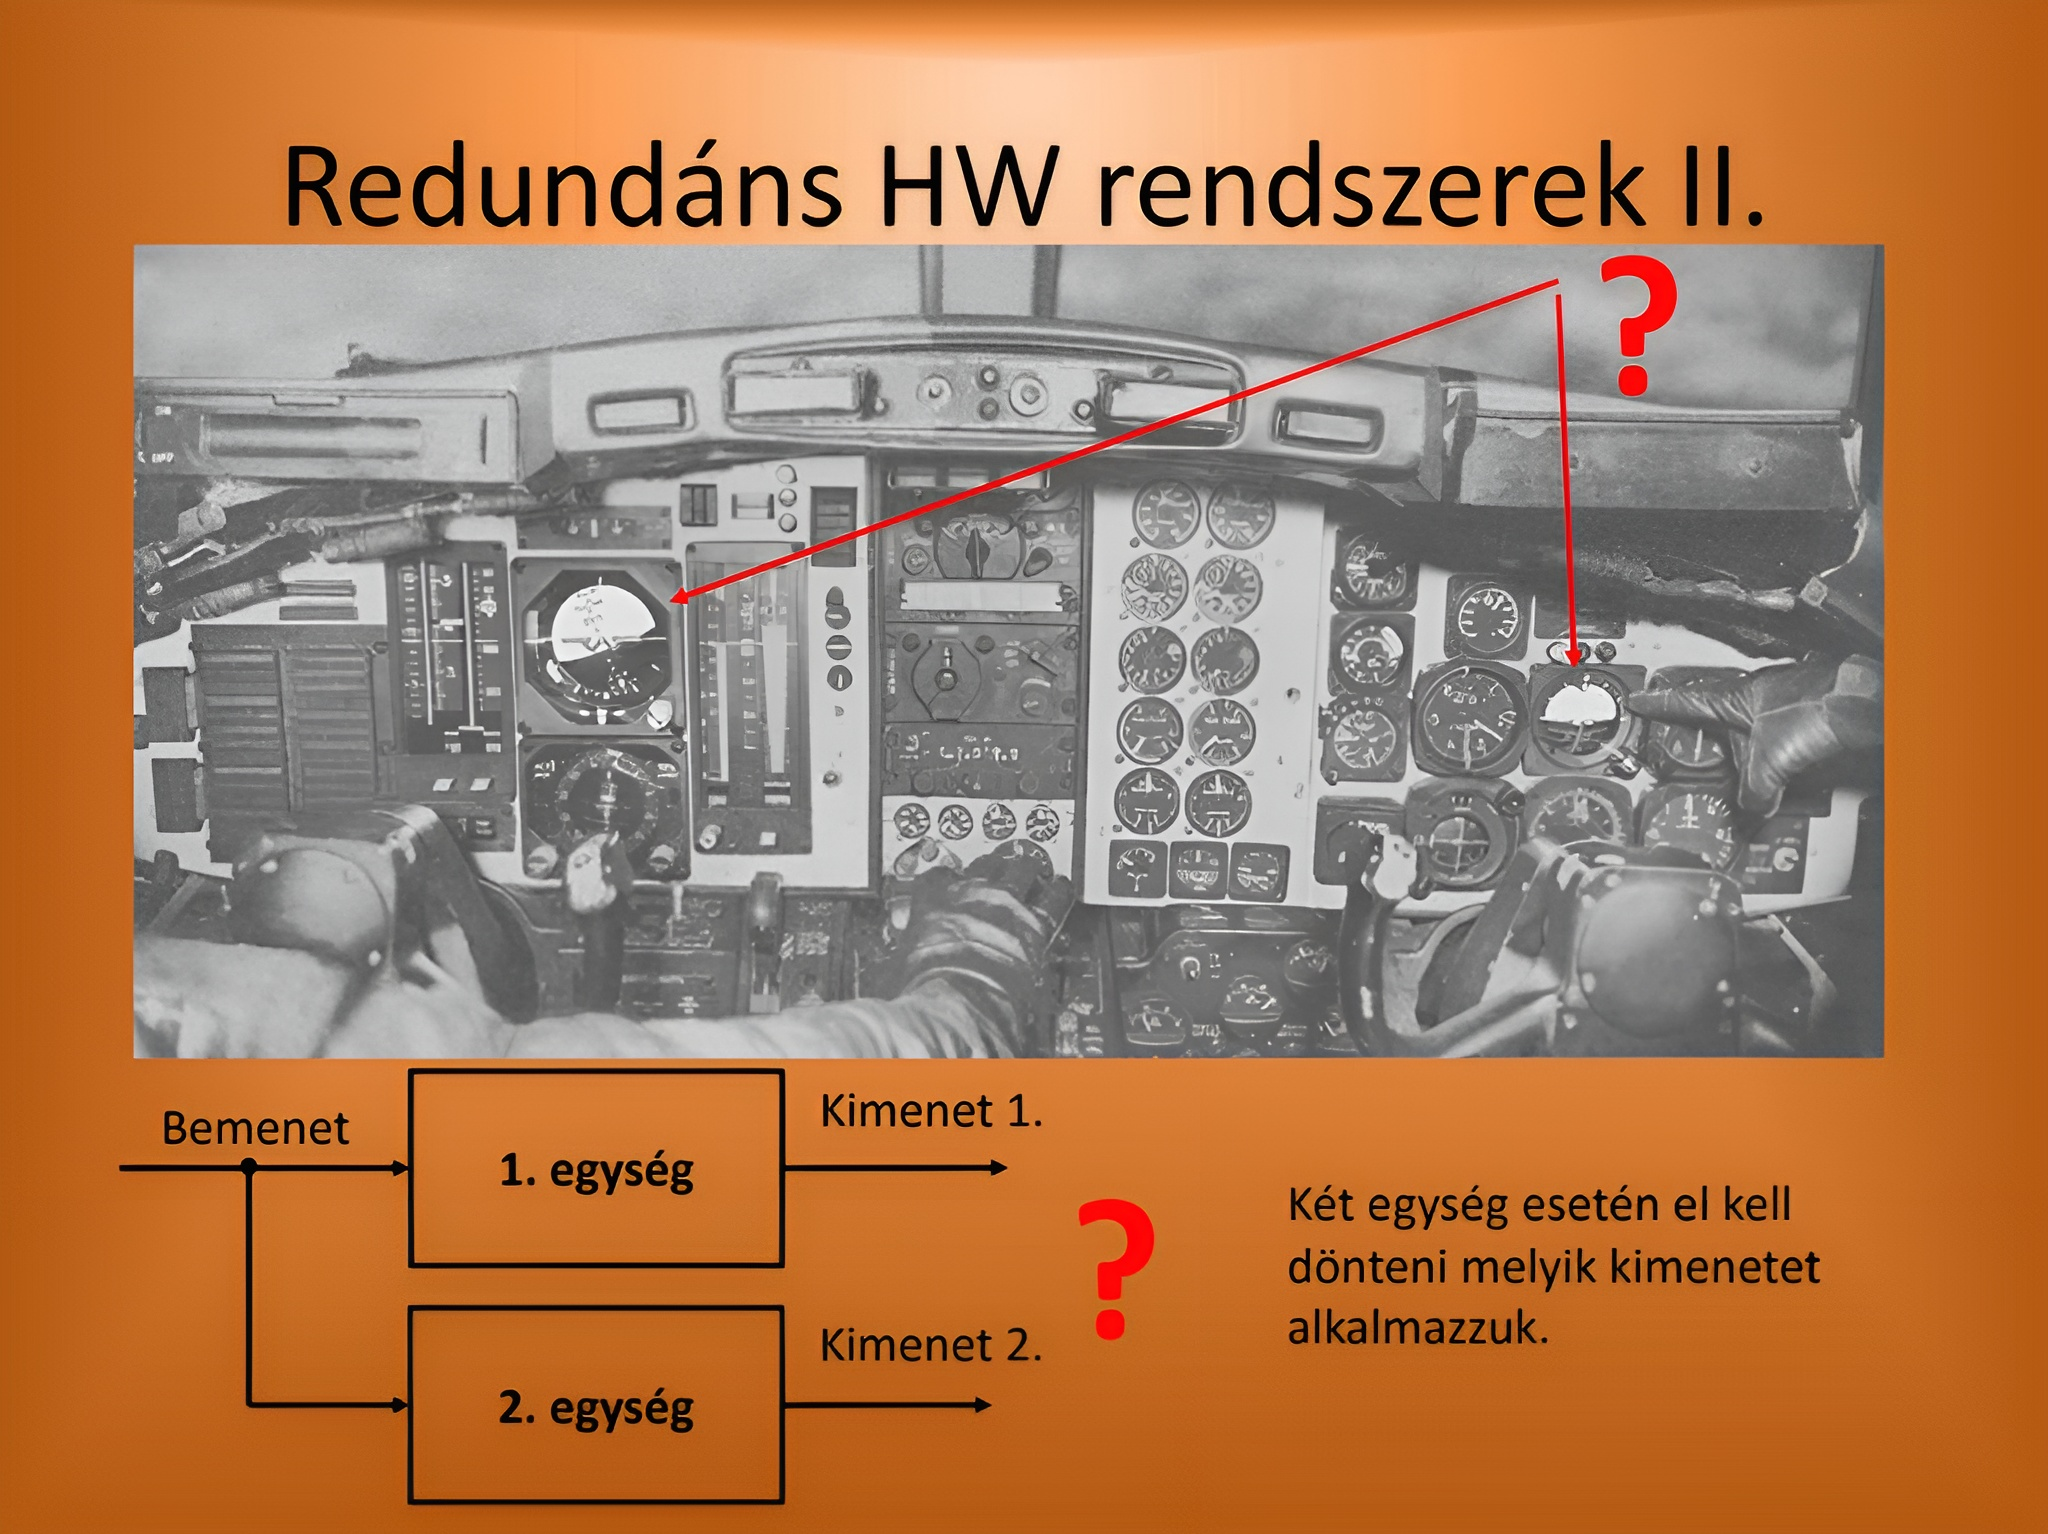
\includegraphics[width=0.7\textwidth]{kep/kep4.png}
    \caption{Redundáns HW rendszerek II. - 2 egységből álló rendszer}
    \label{fig:kep4}
\end{figure}

\begin{figure}[H]
    \centering
    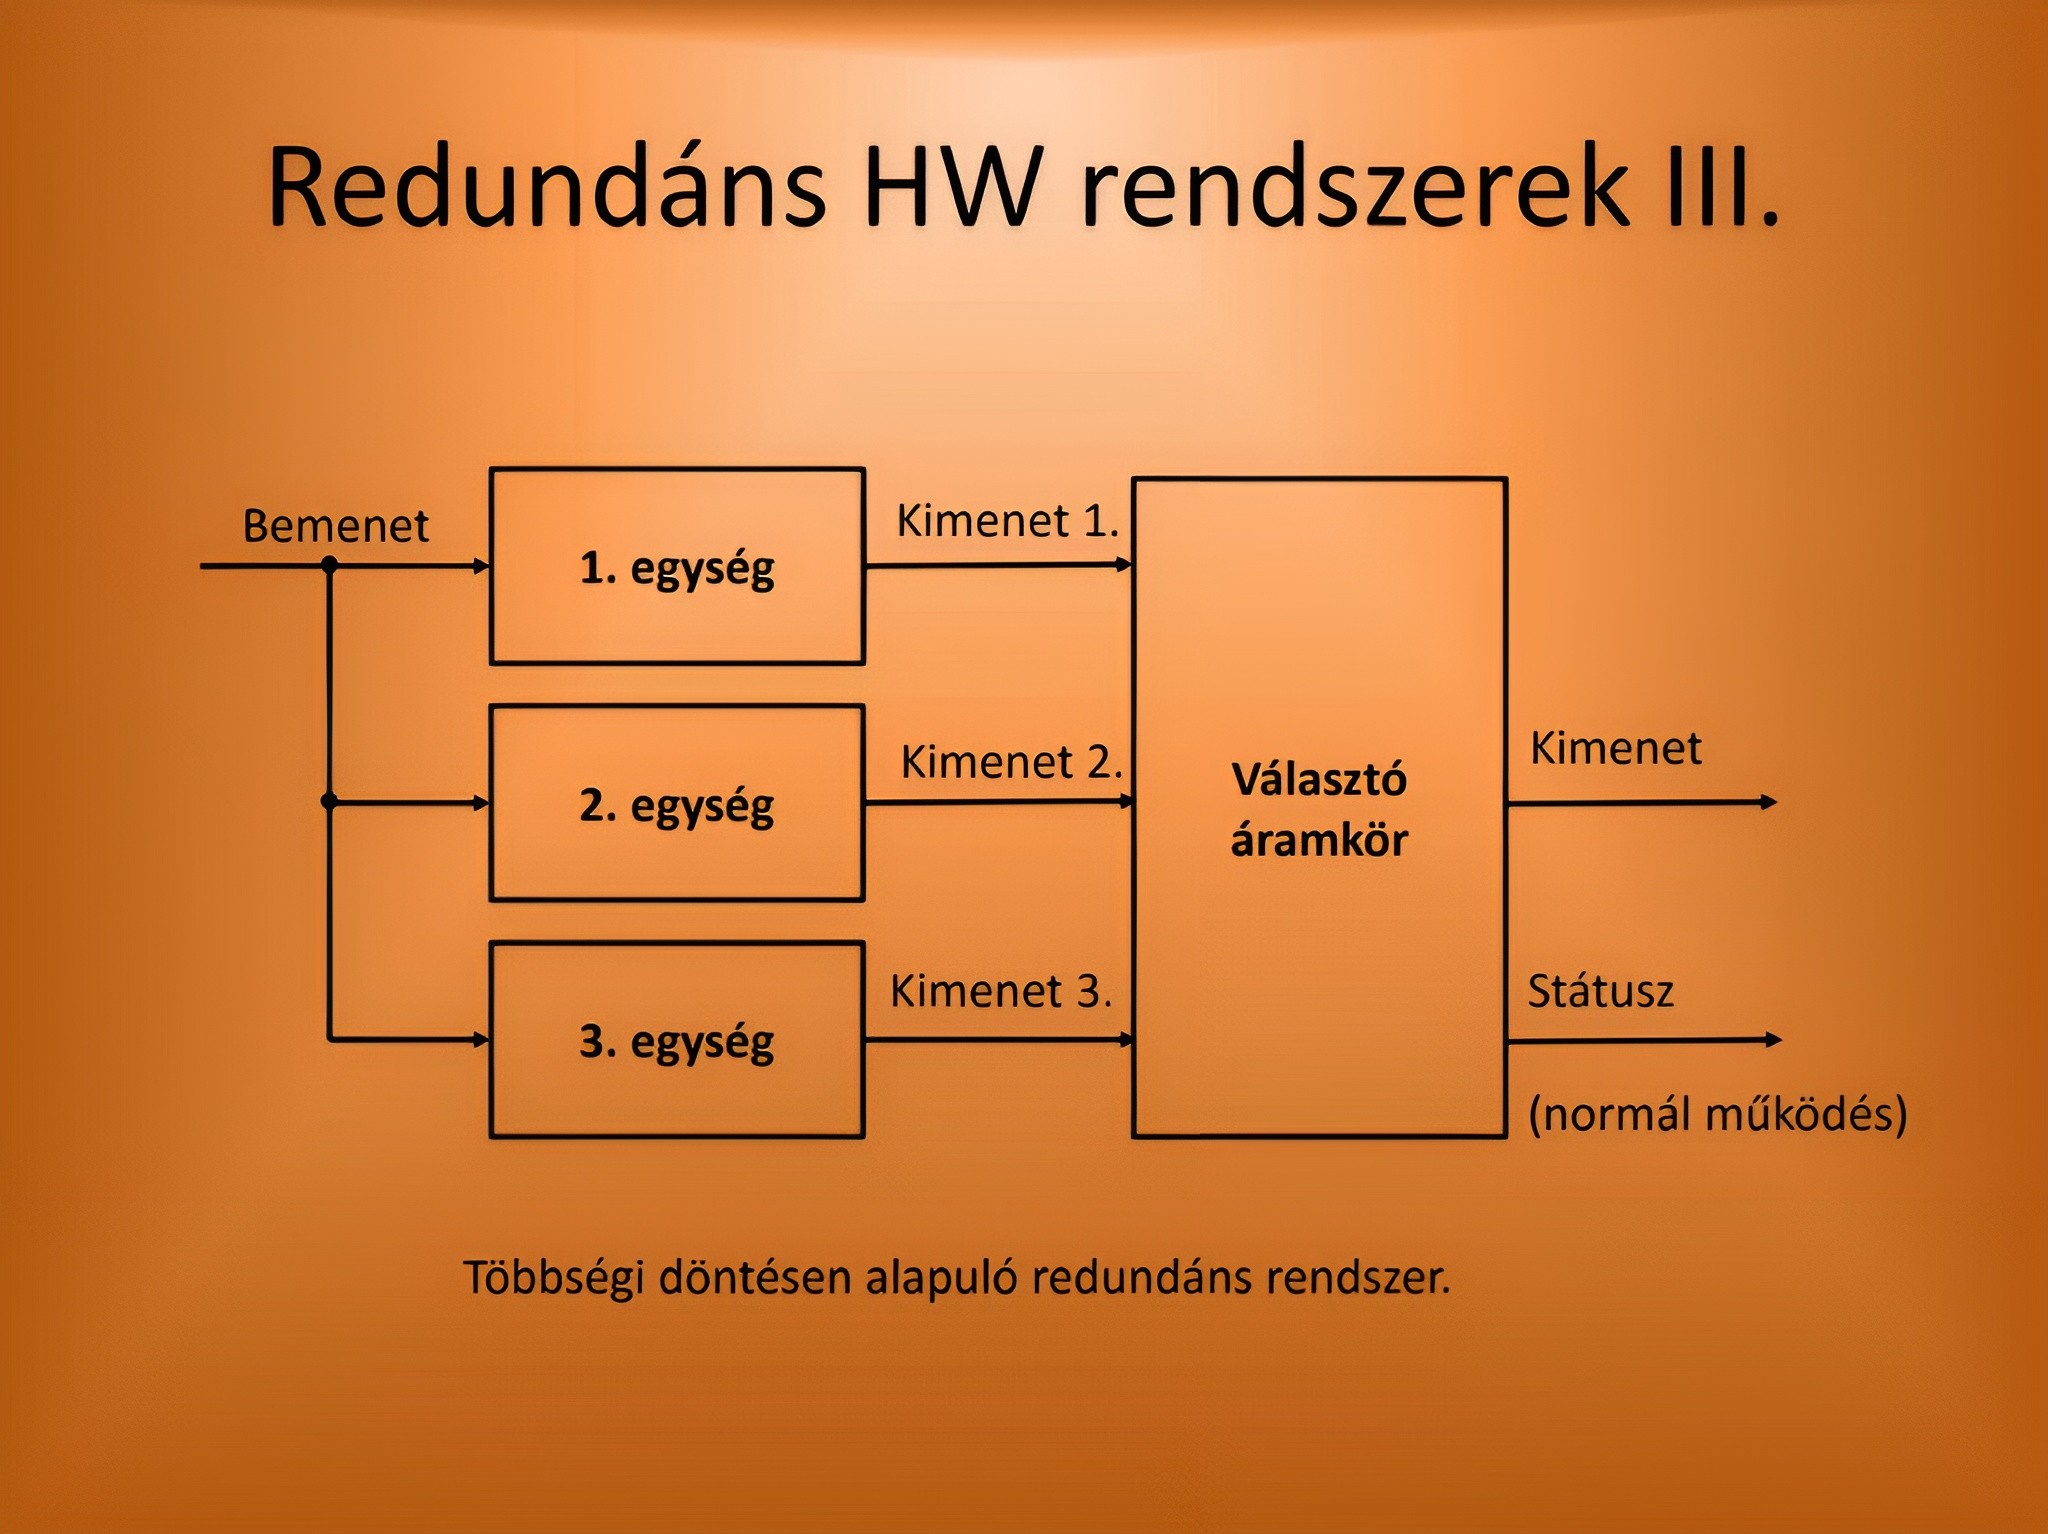
\includegraphics[width=0.7\textwidth]{kep/kep5.png}
    \caption{Redundáns HW rendszerek III. - 3 egységből álló rendszer}
    \label{fig:kep5}
\end{figure}

\begin{figure}[H]
    \centering
    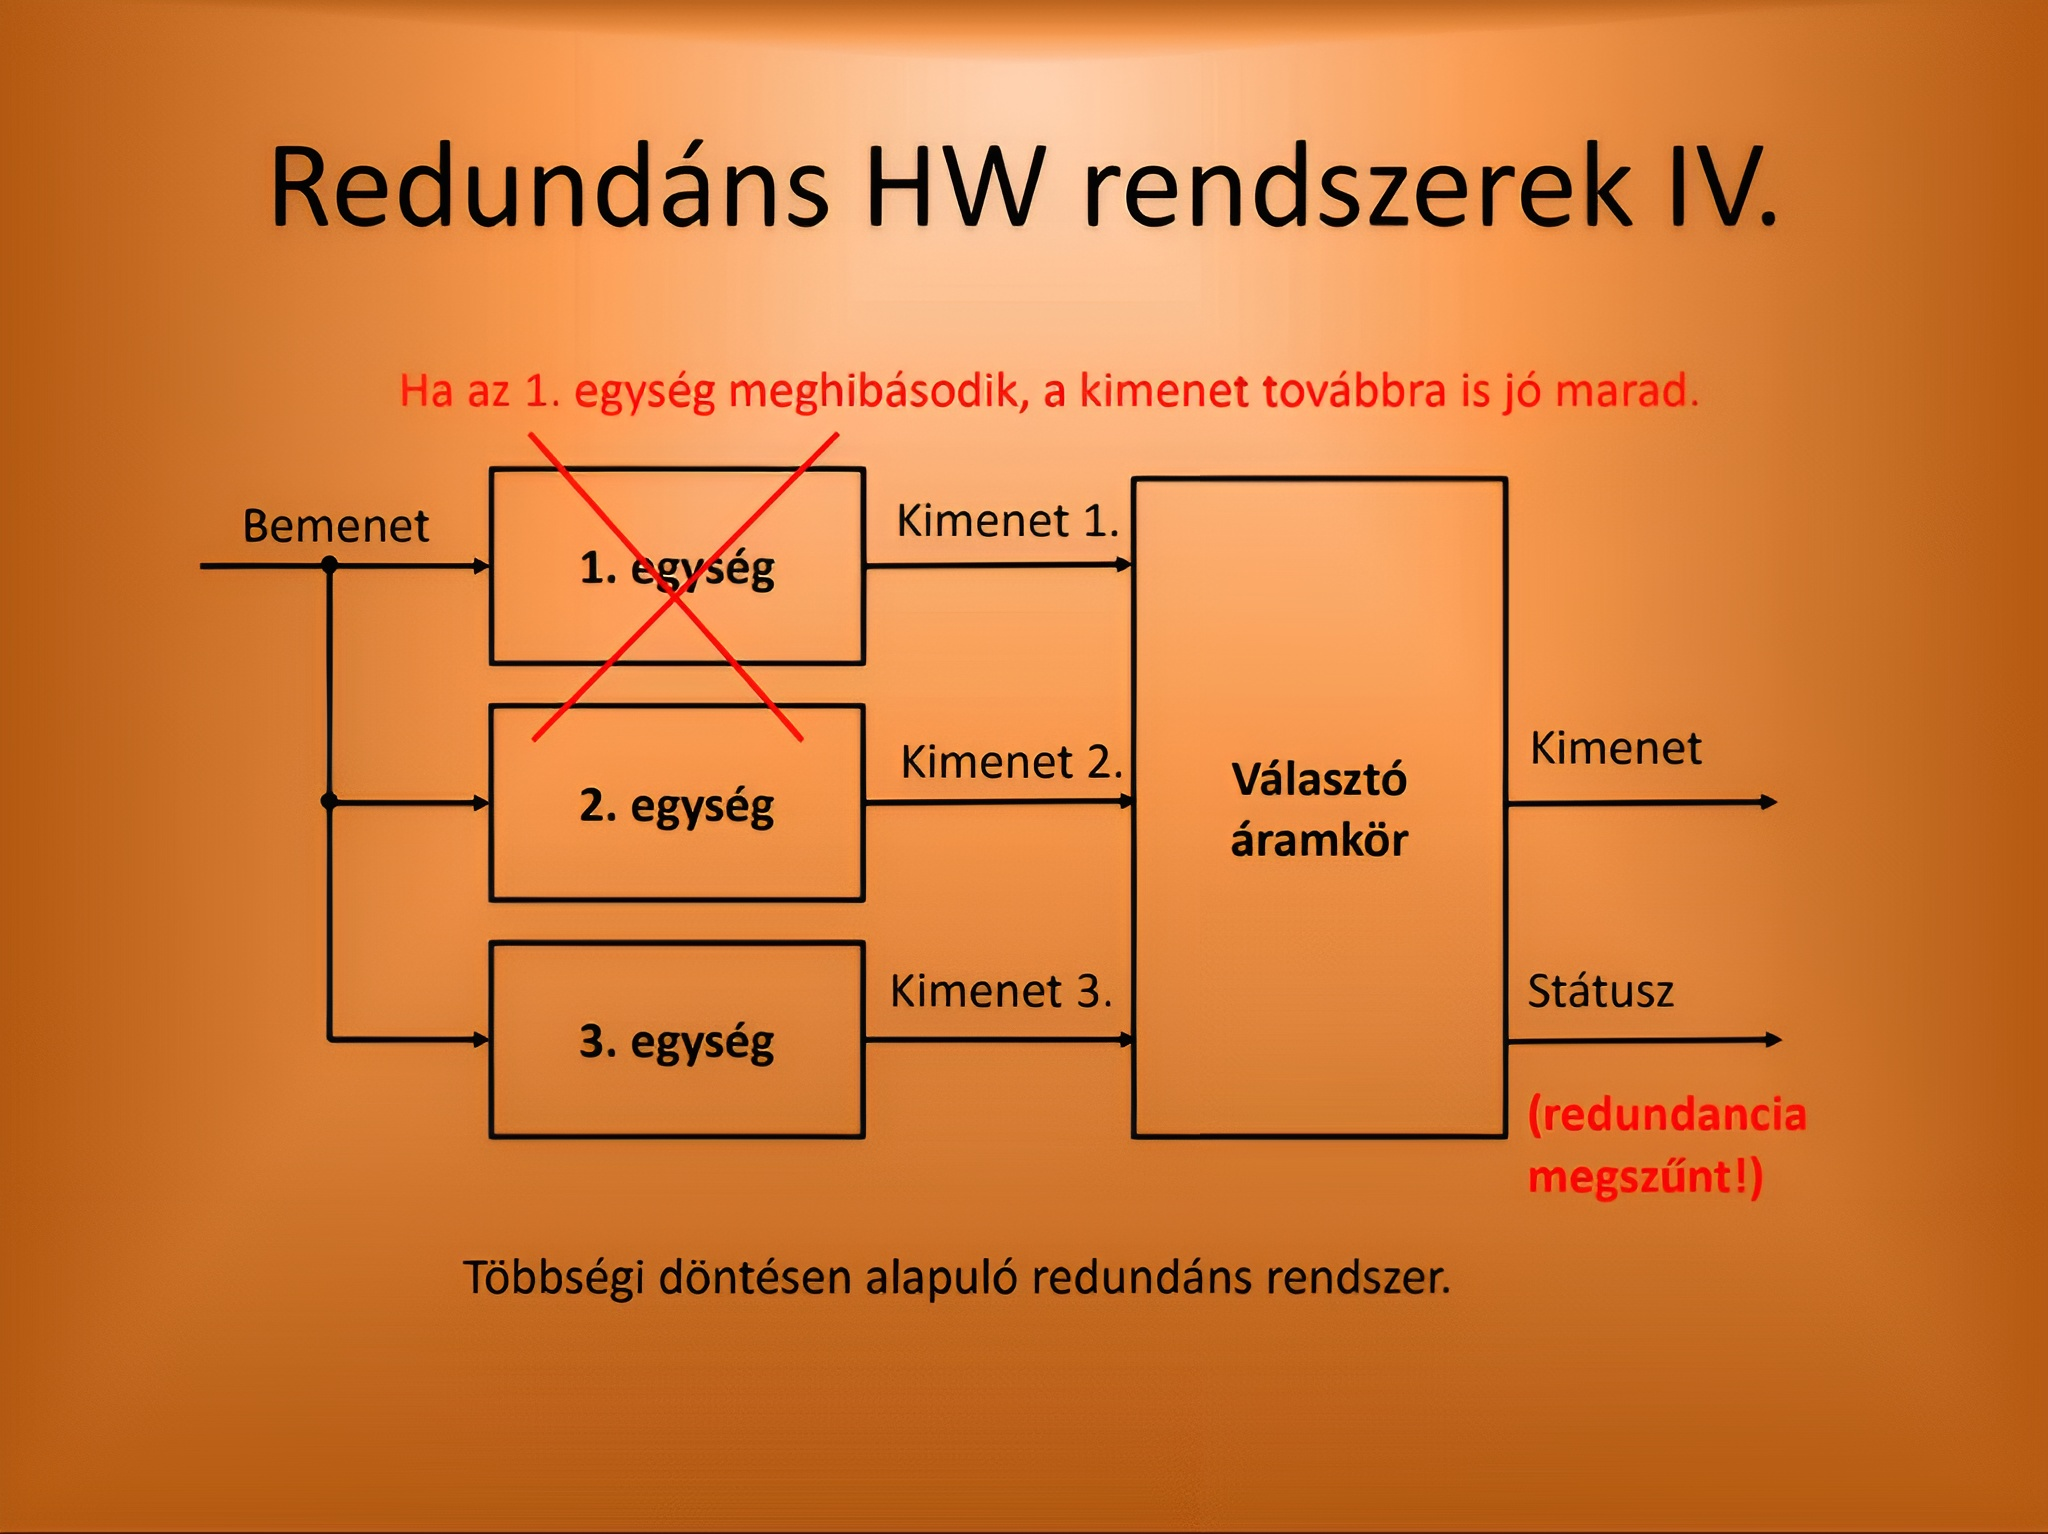
\includegraphics[width=0.7\textwidth]{kep/kep6.png}
    \caption{Redundáns HW rendszerek IV. - 3 egységből álló rendszer meghibásodása}
    \label{fig:kep6}
\end{figure}

\section{Összetett hibák sorozatára való felkészülés}

\begin{itemize}
    \item Több jeladó használata, ha valamelyik elromlik, a többi van használatban.
    \item \textbf{De melyik romlott el, hogy lehet meghatározni?} Például mindenből 3db, vagy másik adatokból következtetni rá, hogy valami gond van.
    \item \textbf{Hogy derül ki, ha valami rossz?} Ha az 1. egység meghibásodik, a kimenet is rossz lesz. Másik körülményt figyelembe véve rá lehet jönni, hogy az az érték nem felel meg a valóságnak.
    \item \textbf{Ha meg van kettőzve a mérés, melyiknek van igaza?} Nem derül ki.
\end{itemize}

\section{Megoldás összetett hibákra}

\begin{figure}[H]
    \centering
    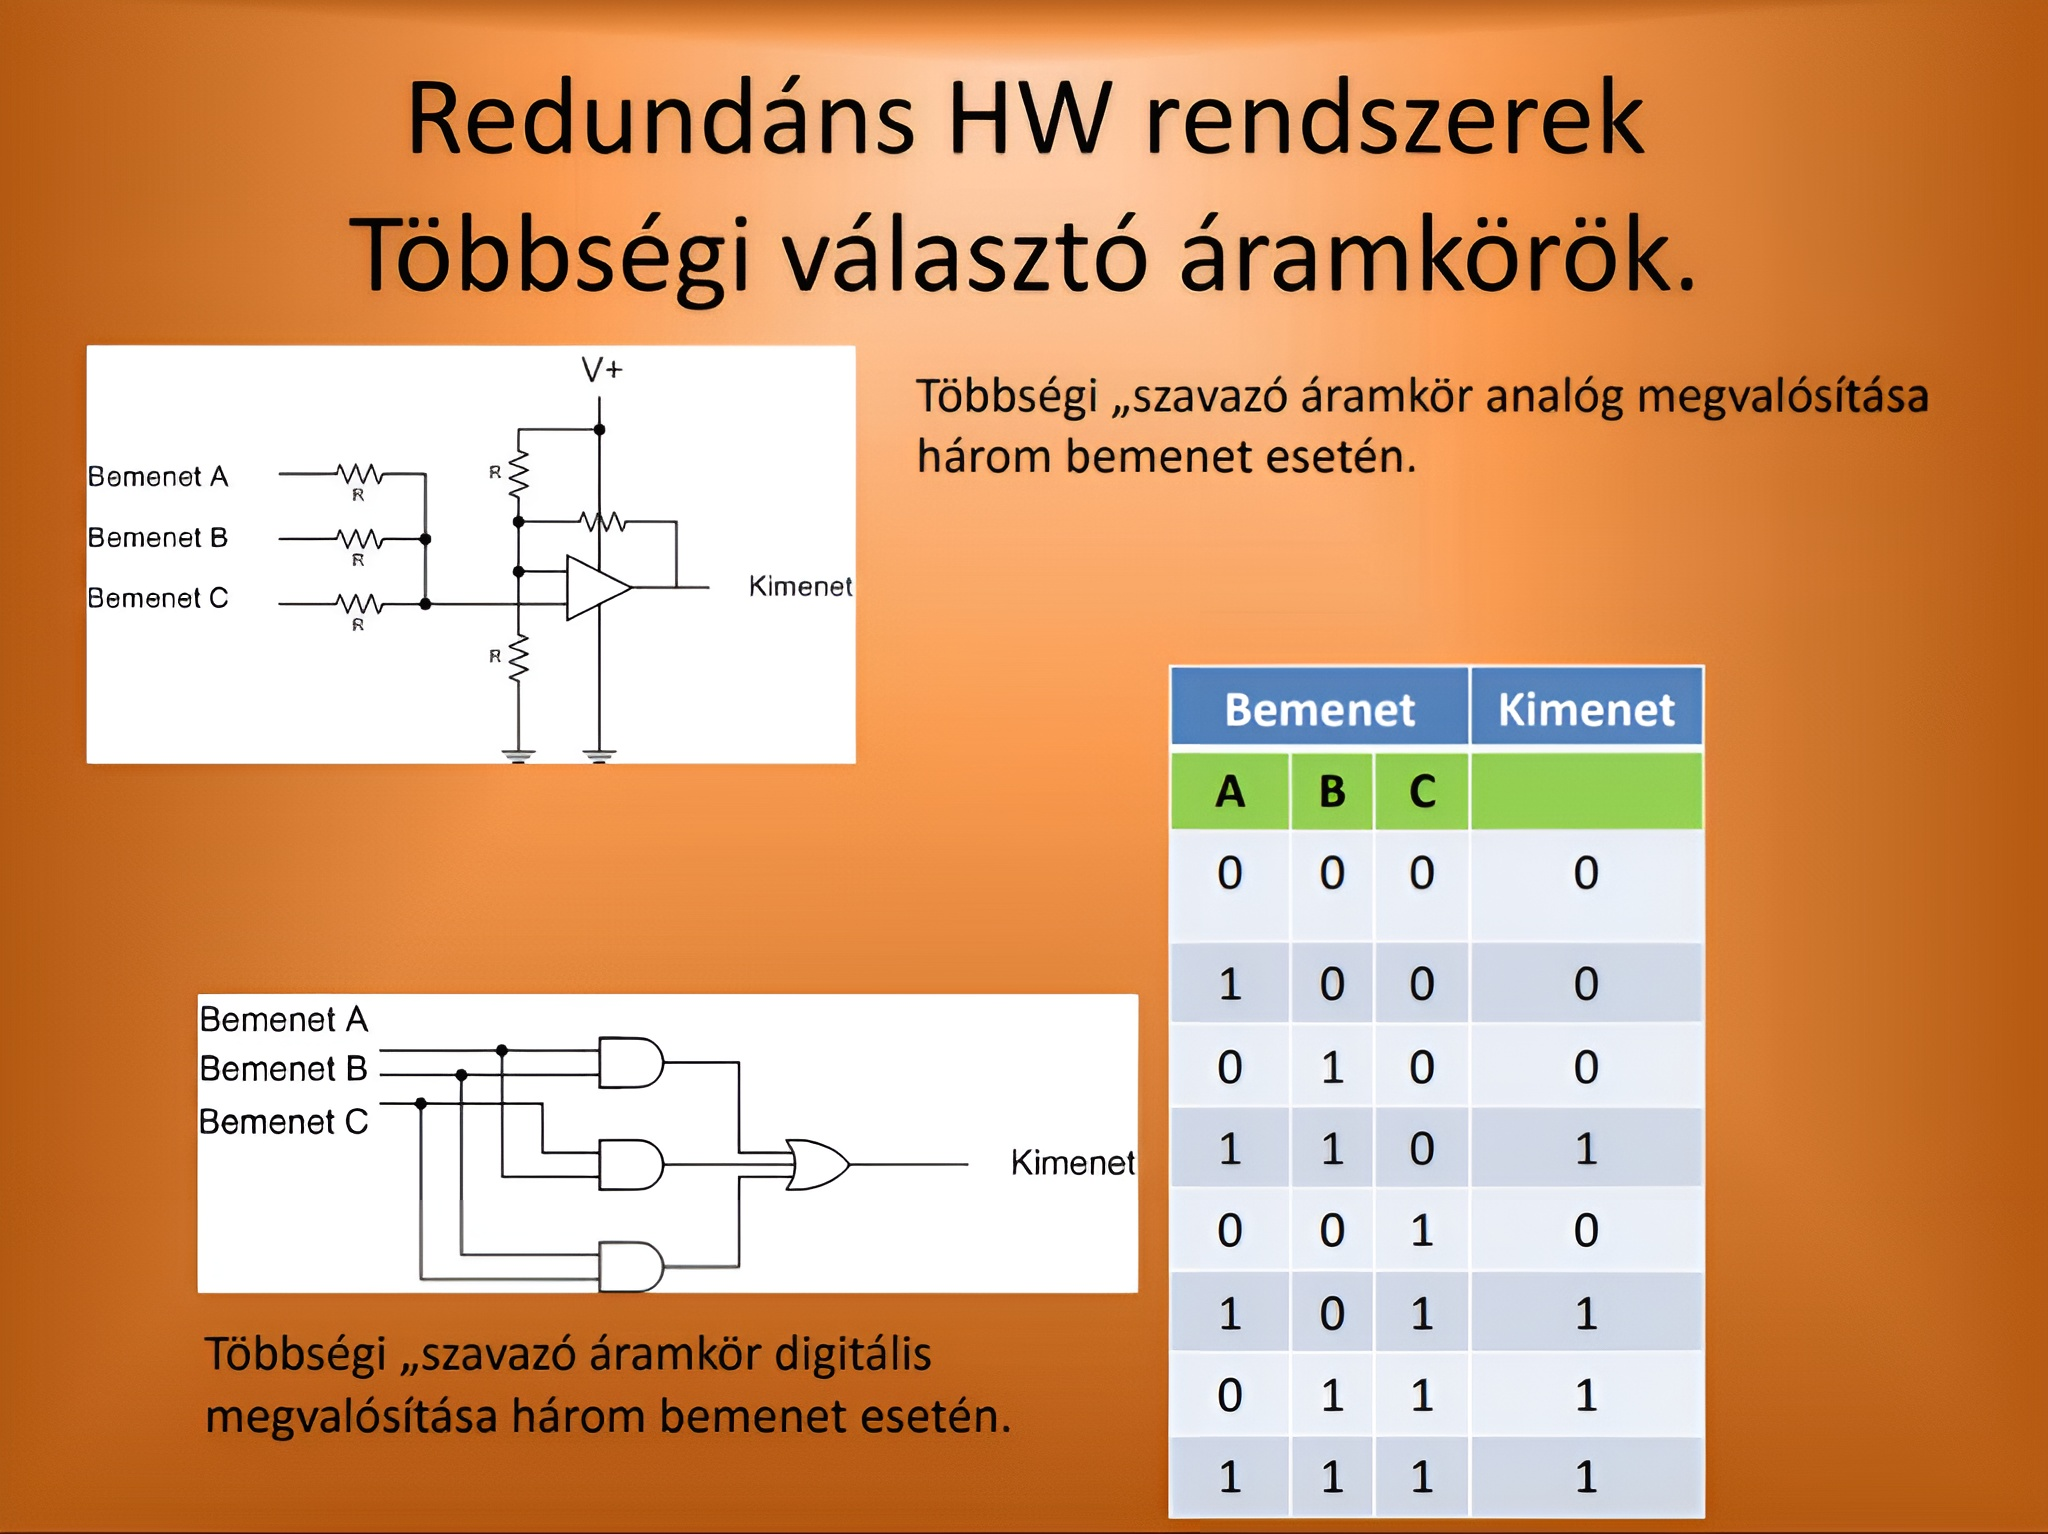
\includegraphics[width=0.7\textwidth]{kep/kep7.png}
    \caption{Redundáns HW rendszerek - Többségi választó áramkörök}
    \label{fig:kep7}
\end{figure}

\begin{itemize}
    \item \textbf{Minimum 3 redundáns egységre van szükség,} mert 2 közül nem lehet eldönteni melyik működik helyesen.
    \item Ha van 3 egység, egy \textbf{választó áramkör tudja ezeket felügyelni,} és megadni a helyes kimentetet.
    \item Ha a 3 egységből 1 eltérő eredményt ad, azt a kimenetet lekapcsolja és a maradék kettő közül választ egyet a végleges kimenetre, hibajelzés mellett.
    \item Ha 2 egység hibásodik meg, az utolsó működőképes egység jelét kapcsolja be, de hibával jelzi, hogy az érték nem megbízható.
    \item Az egységek nem feltétlenül ugyanazok a dobozok többszörözve, hanem például hasonló, de nem ugyanolyan készülékek, amik ugyanazt a feladatkört látják el.
    \item Például hiba lehet, ha 1 szenzort használnak és ezt az egyet értékelik ki 3 egységgel.
    \item Többségi választó áramkör használata: nagyon egyszerű áramkör, nem valószínű a meghibásodása. Létezik analóg és digitális megvalósítása.
\end{itemize}

\textbf{\textit{Két egység az egy kétség.}}

\begin{figure}[H]
    \centering
    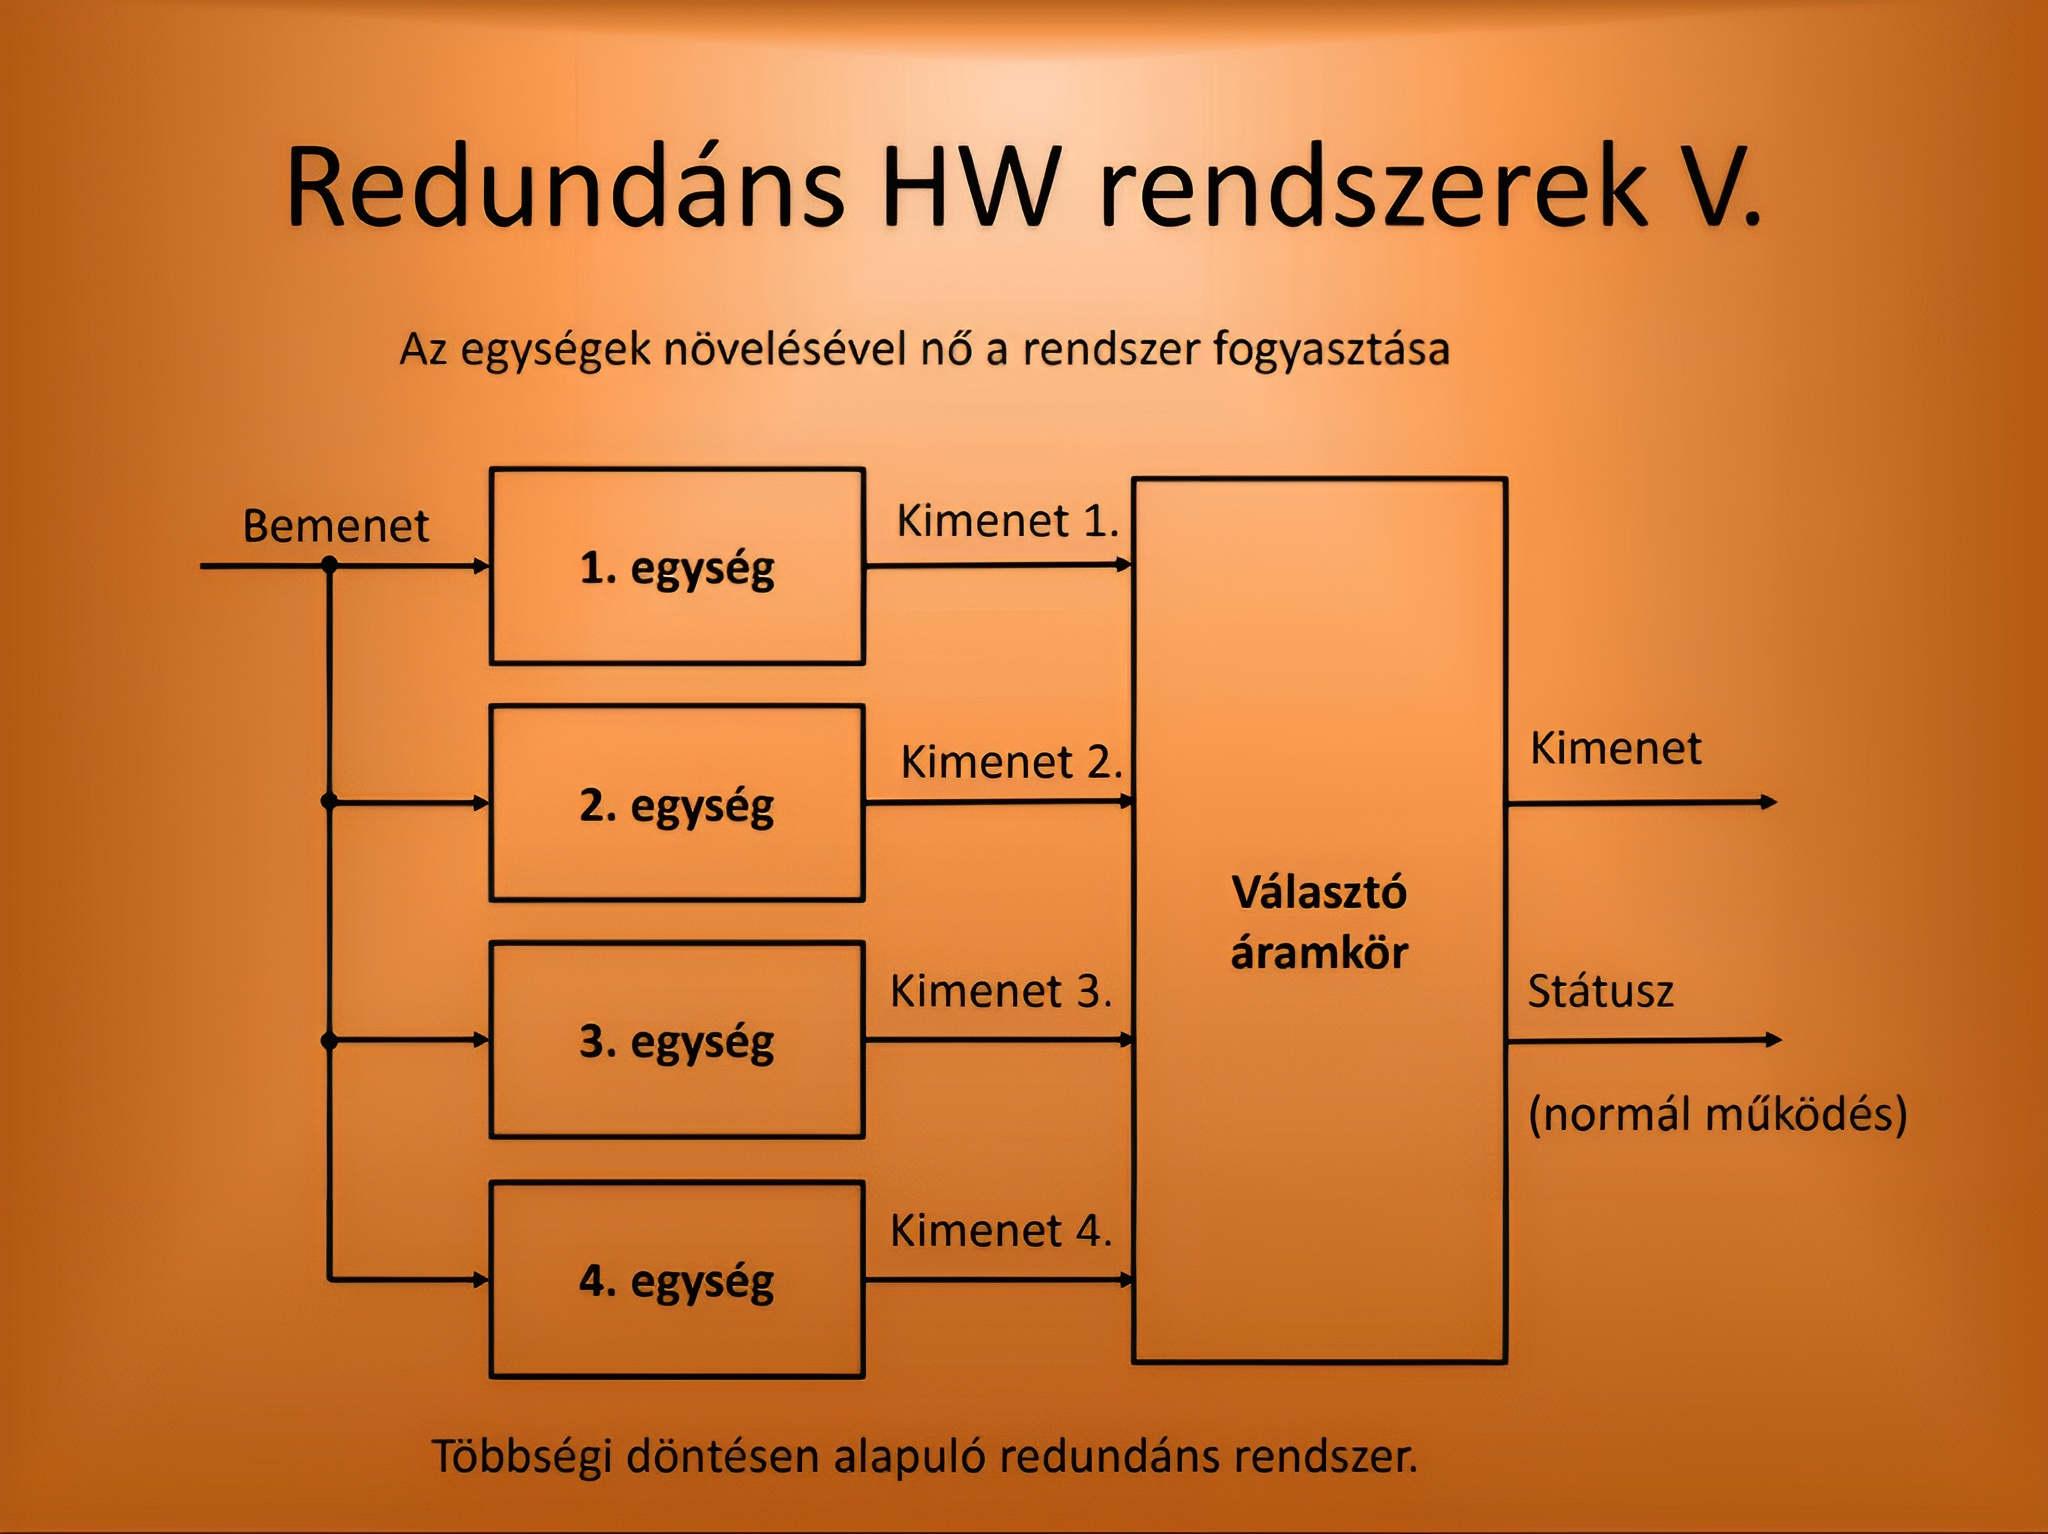
\includegraphics[width=0.7\textwidth]{kep/kep8.png}
    \caption{Redundáns HW rendszerek V. - 4 egységből álló rendszer}
    \label{fig:kep8}
\end{figure}

\begin{figure}[H]
    \centering
    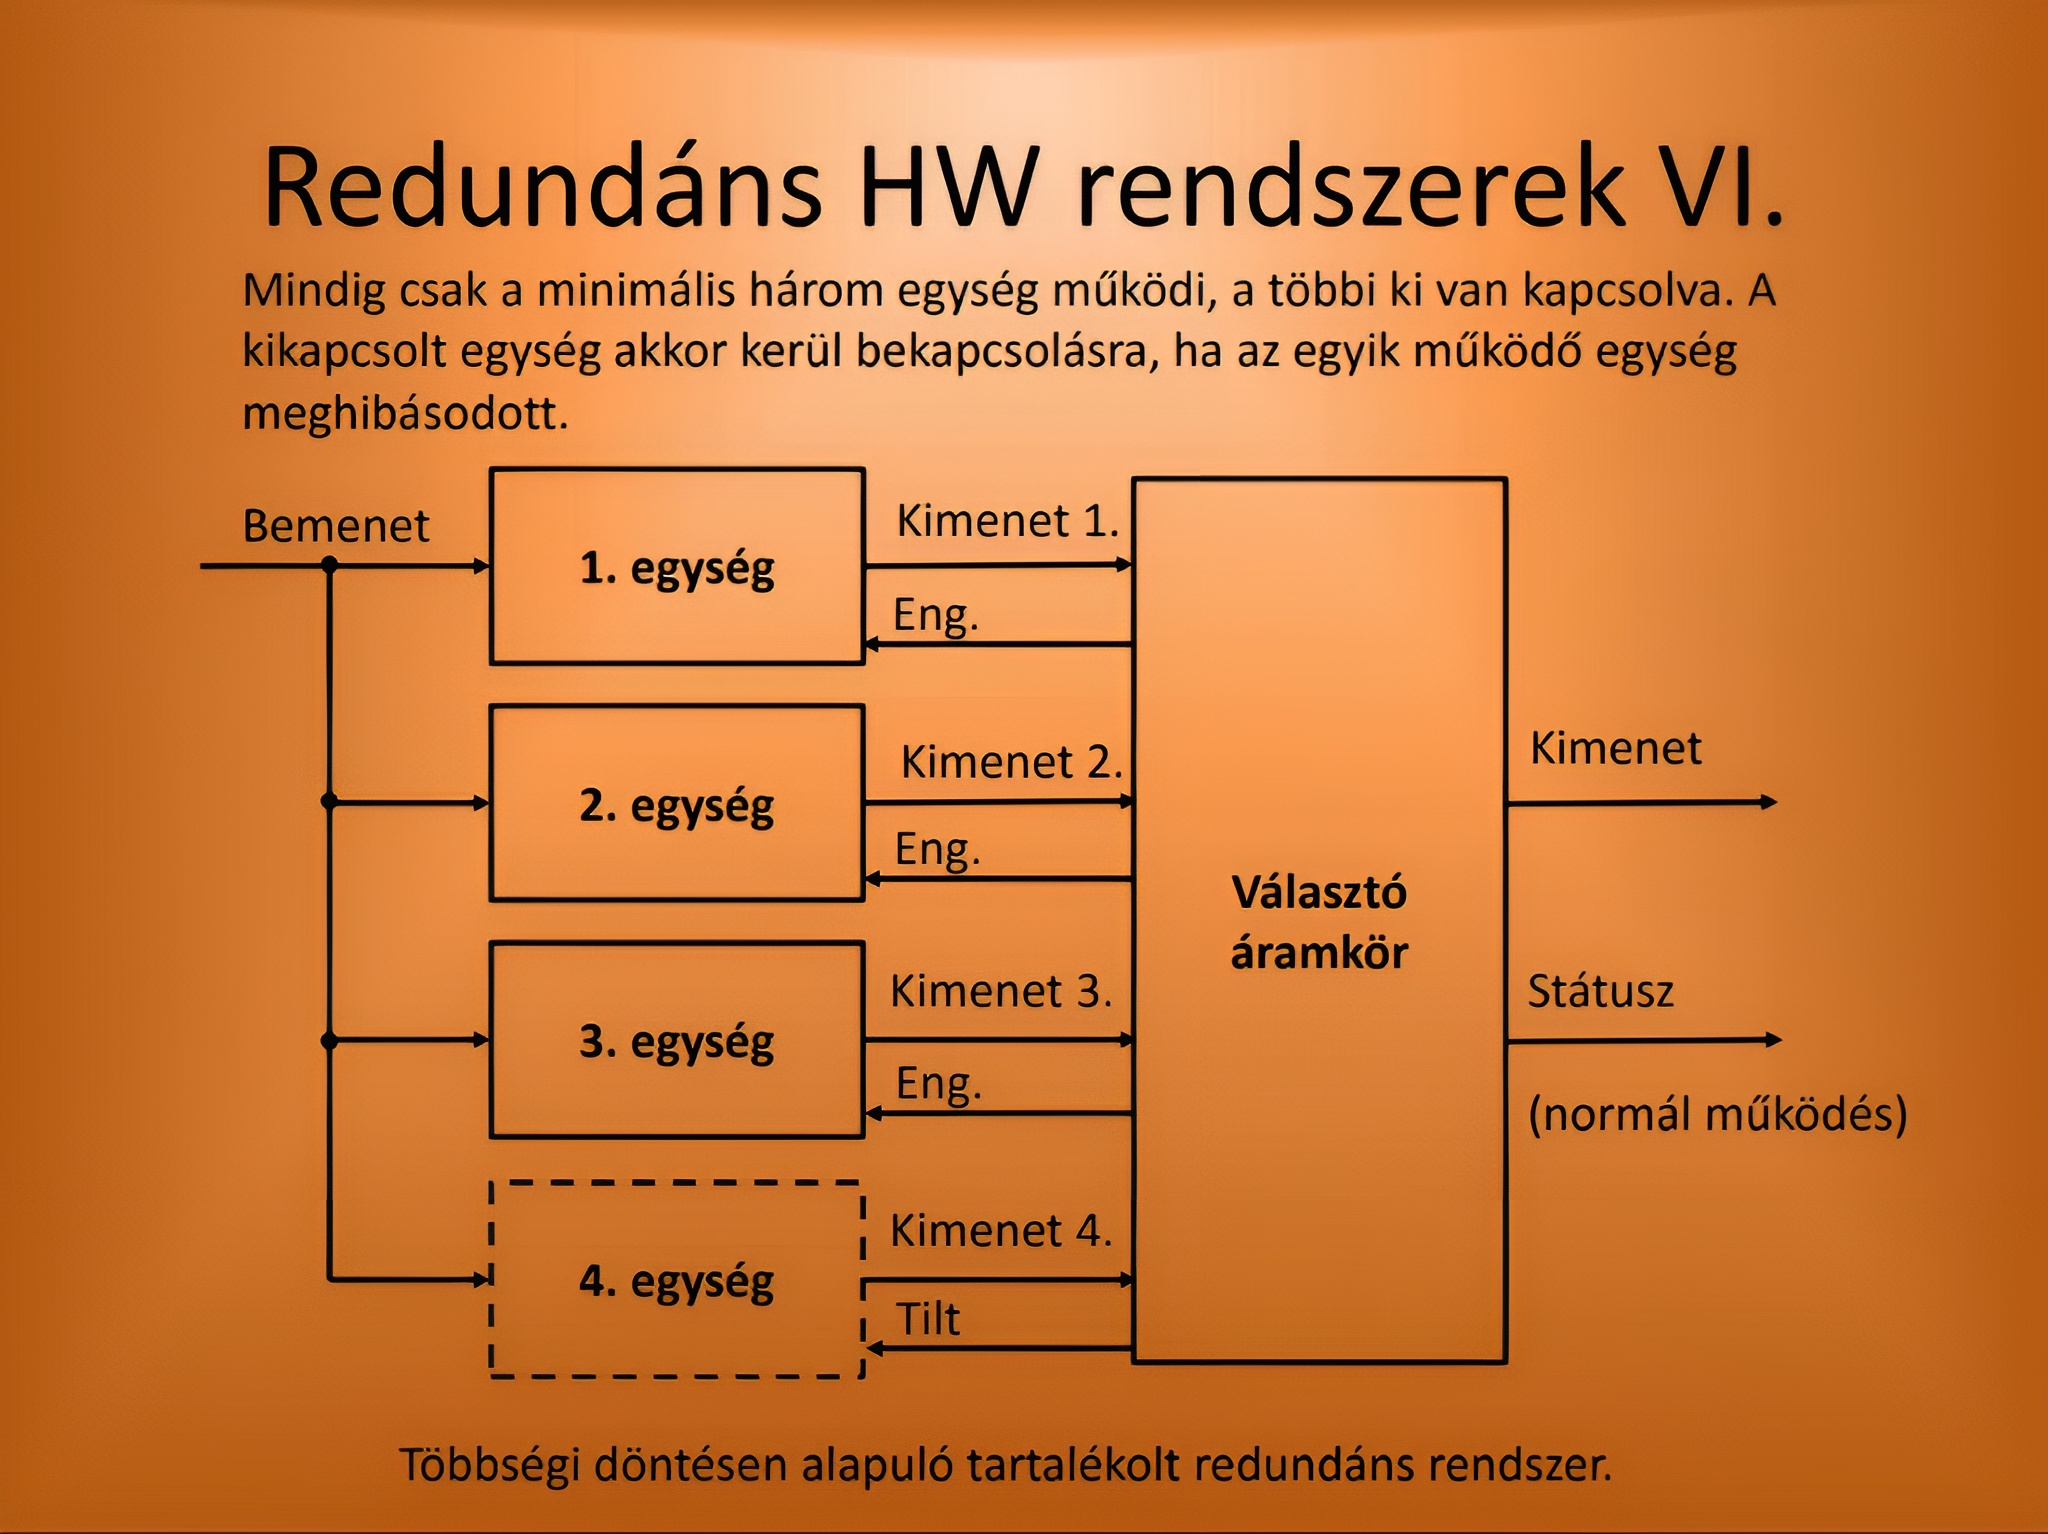
\includegraphics[width=0.7\textwidth]{kep/kep9.png}
    \caption{Redundáns HW rendszerek VI. - 4 egységből álló rendszer működése}
    \label{fig:kep9}
\end{figure}

\begin{figure}[H]
    \centering
    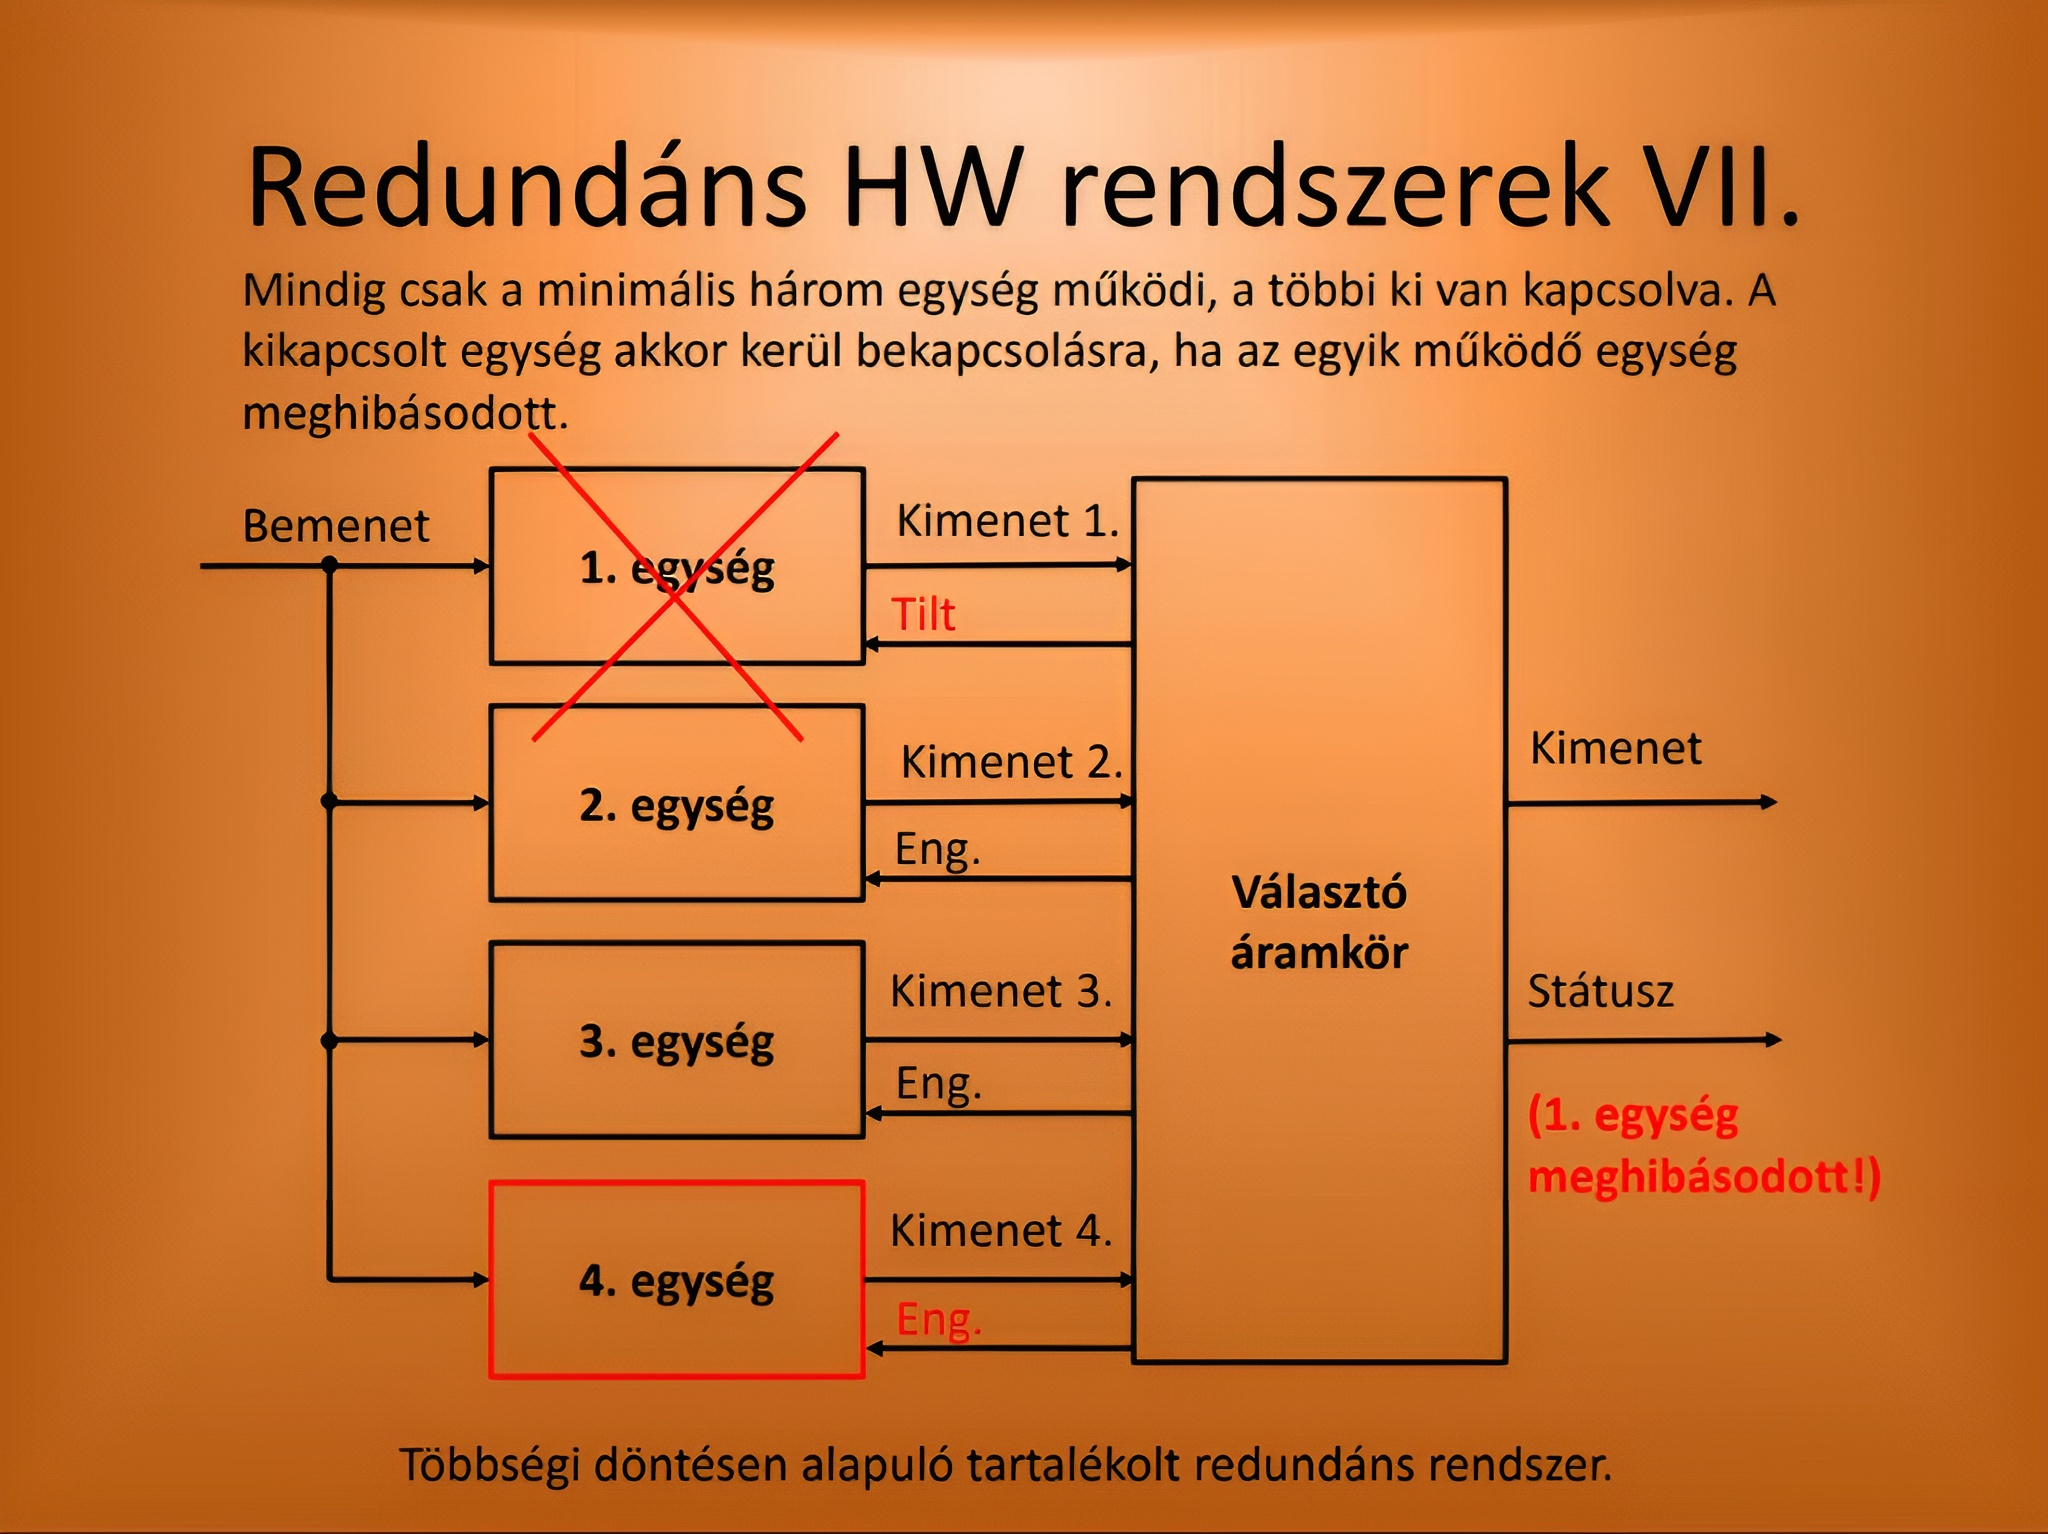
\includegraphics[width=0.7\textwidth]{kep/kep10.png}
    \caption{Redundáns HW rendszerek VII. - 4 egységből álló rendszer meghibásodása}
    \label{fig:kep10}
\end{figure}

\begin{figure}[H]
    \centering
    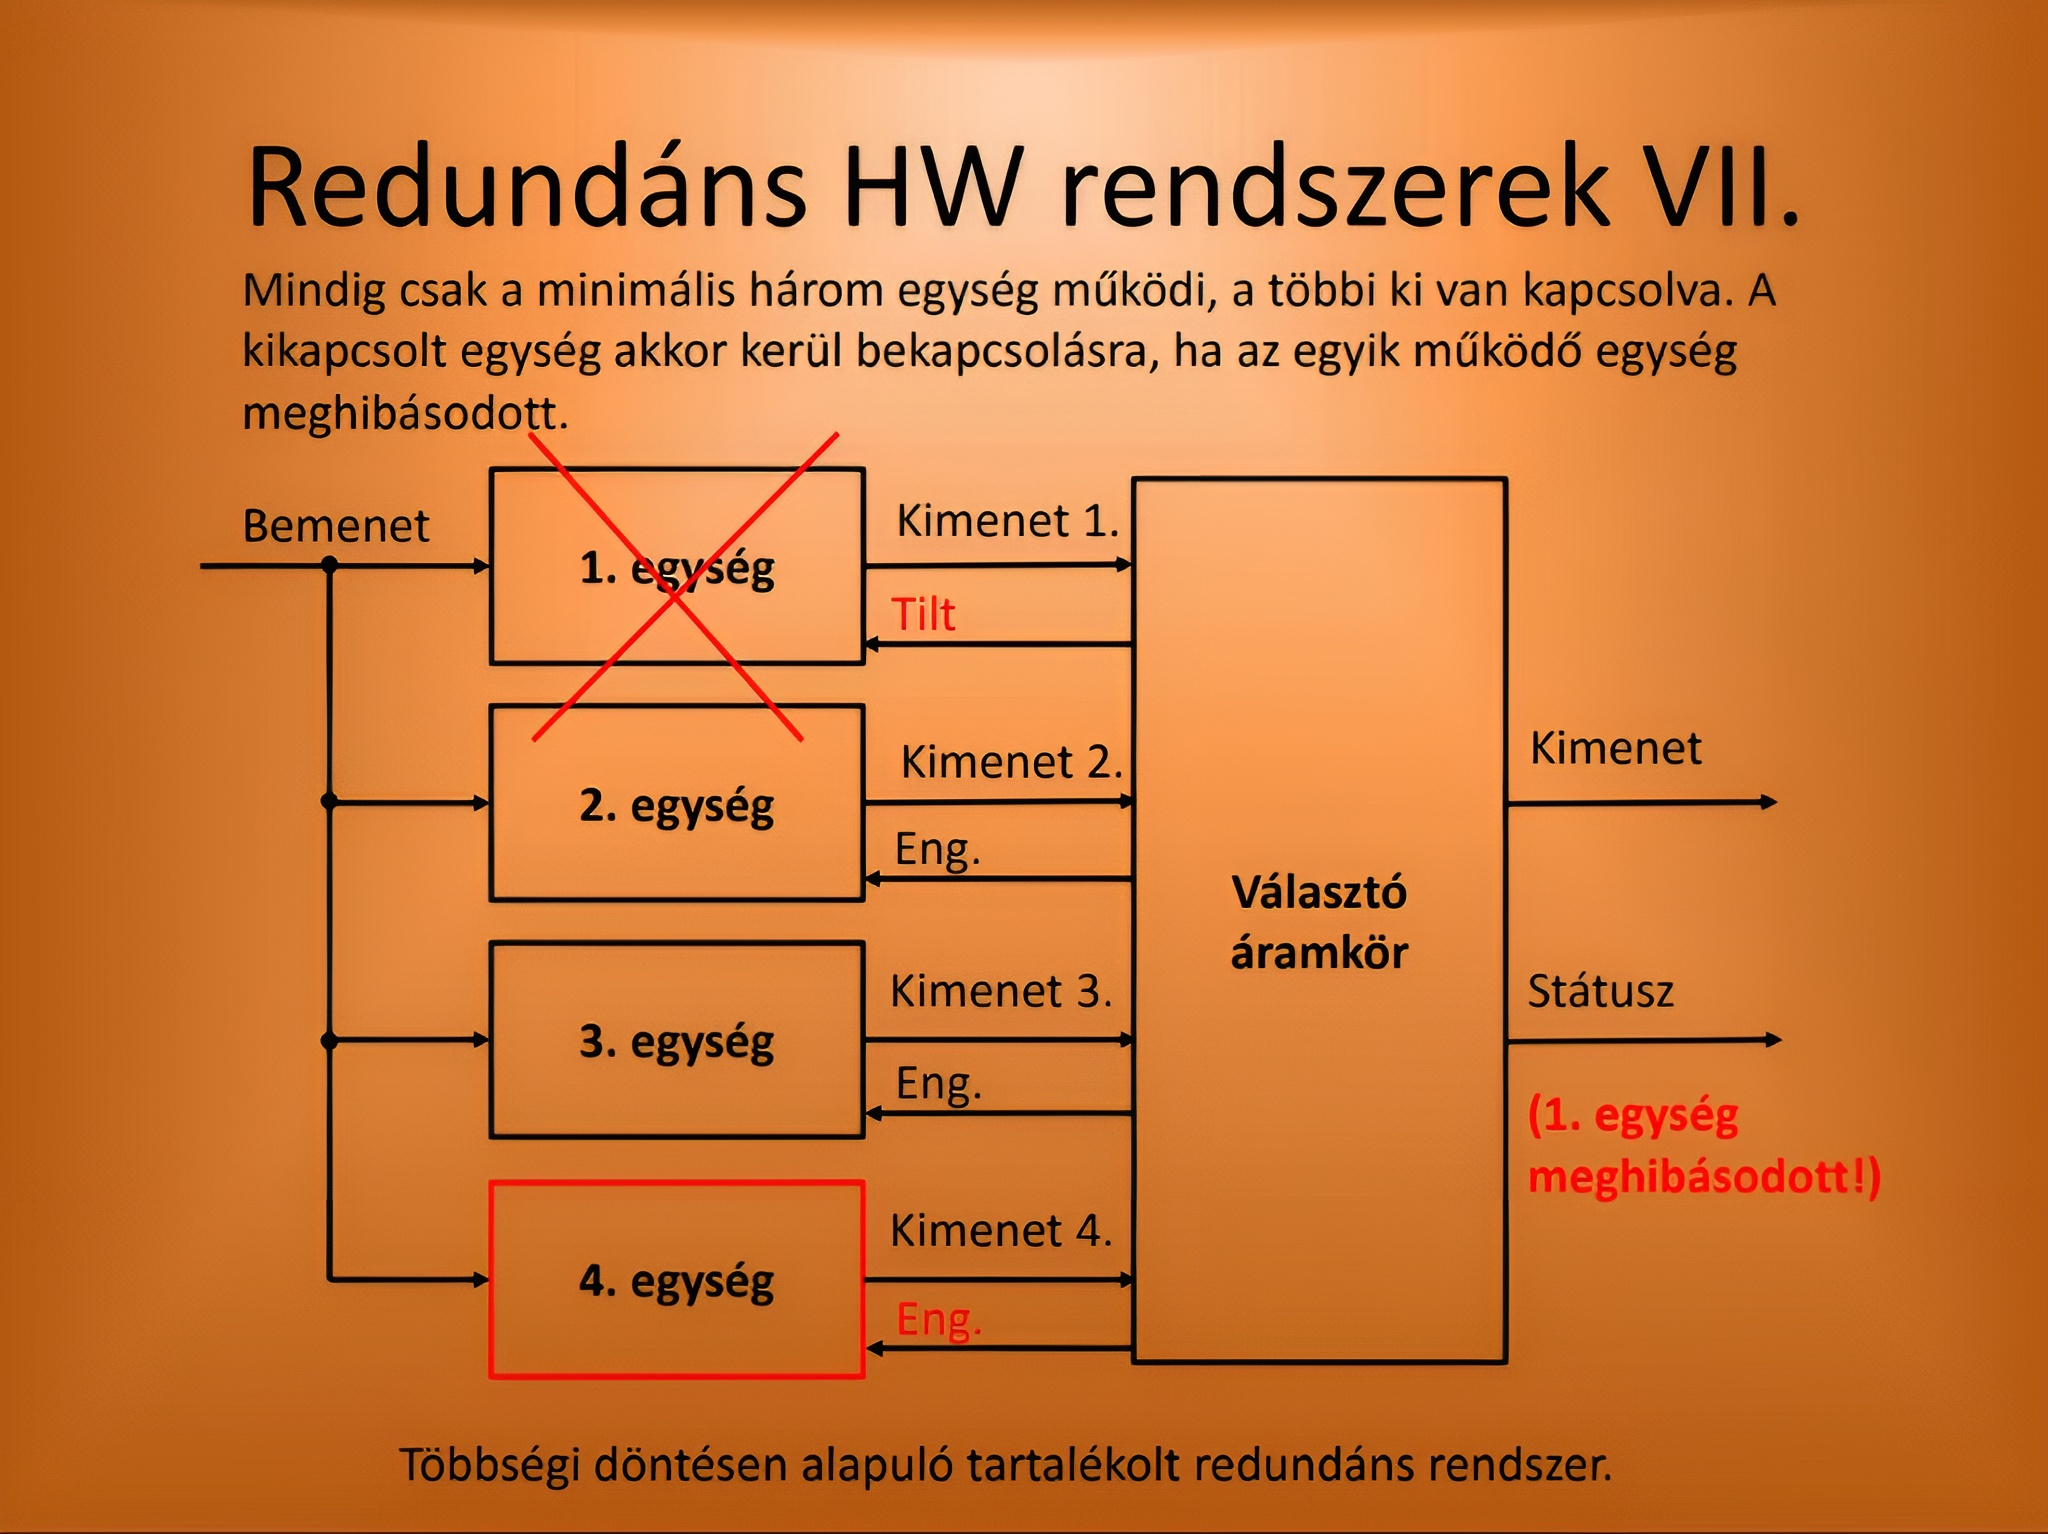
\includegraphics[width=0.7\textwidth]{kep/kep11.png}
    \caption{Redundáns HW rendszerek VIII. - 4 egységből álló rendszer meghibásodása}
    \label{fig:kep11}
\end{figure}

\begin{figure}[H]
    \centering
    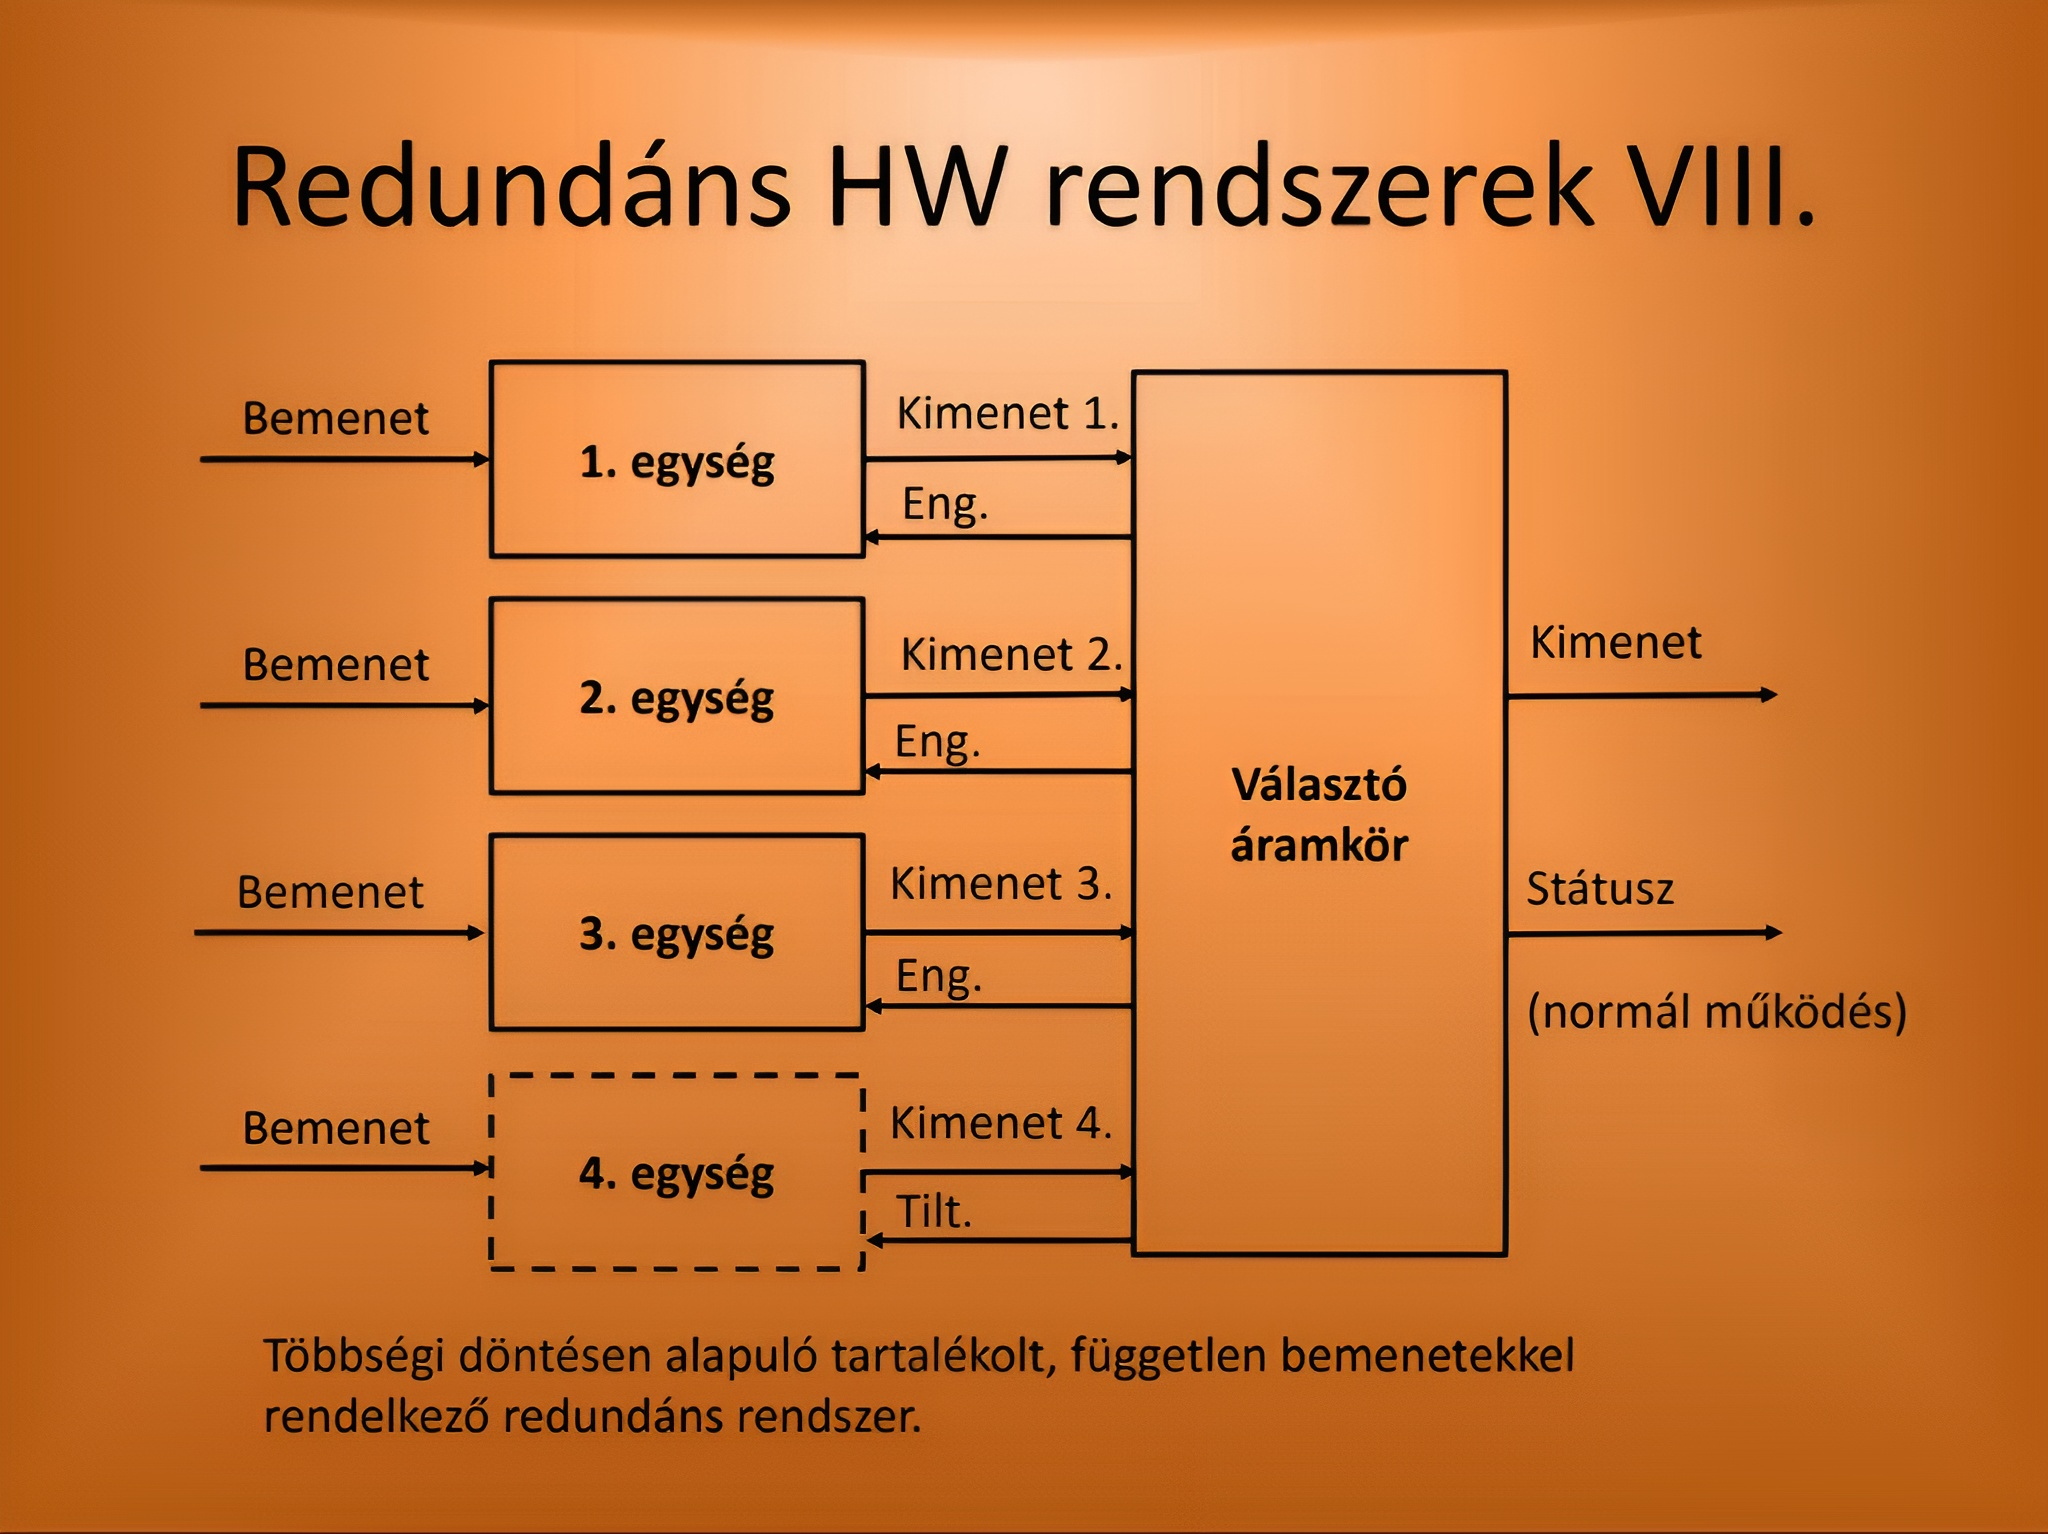
\includegraphics[width=0.7\textwidth]{kep/kep12.png}
    \caption{Redundáns HW rendszerek VIII. - 4 egységből álló rendszer független bemenetekkel}
    \label{fig:kep12}
\end{figure}

\section{Lehetséges megoldások redundáns rendszerek megvalósítására}

\begin{itemize}
    \item 3 egység helyett lehet 4 egységes rendszert használni
    \item 4 egység esetén lehetőség van rá, hogy a negyedik egység alapértelmezetten ki van kapcsolva, csak akkor kap áramot ha egy másik egység meghibásodik, és szükséges lesz a negyedik belépése.
    \item Redundáns egységek mellett egy szenzor helyett redundáns szenzorokat kell használni.
\end{itemize}

\section{Öndiagnosztizáló rendszer}

\begin{figure}[H]
    \centering
    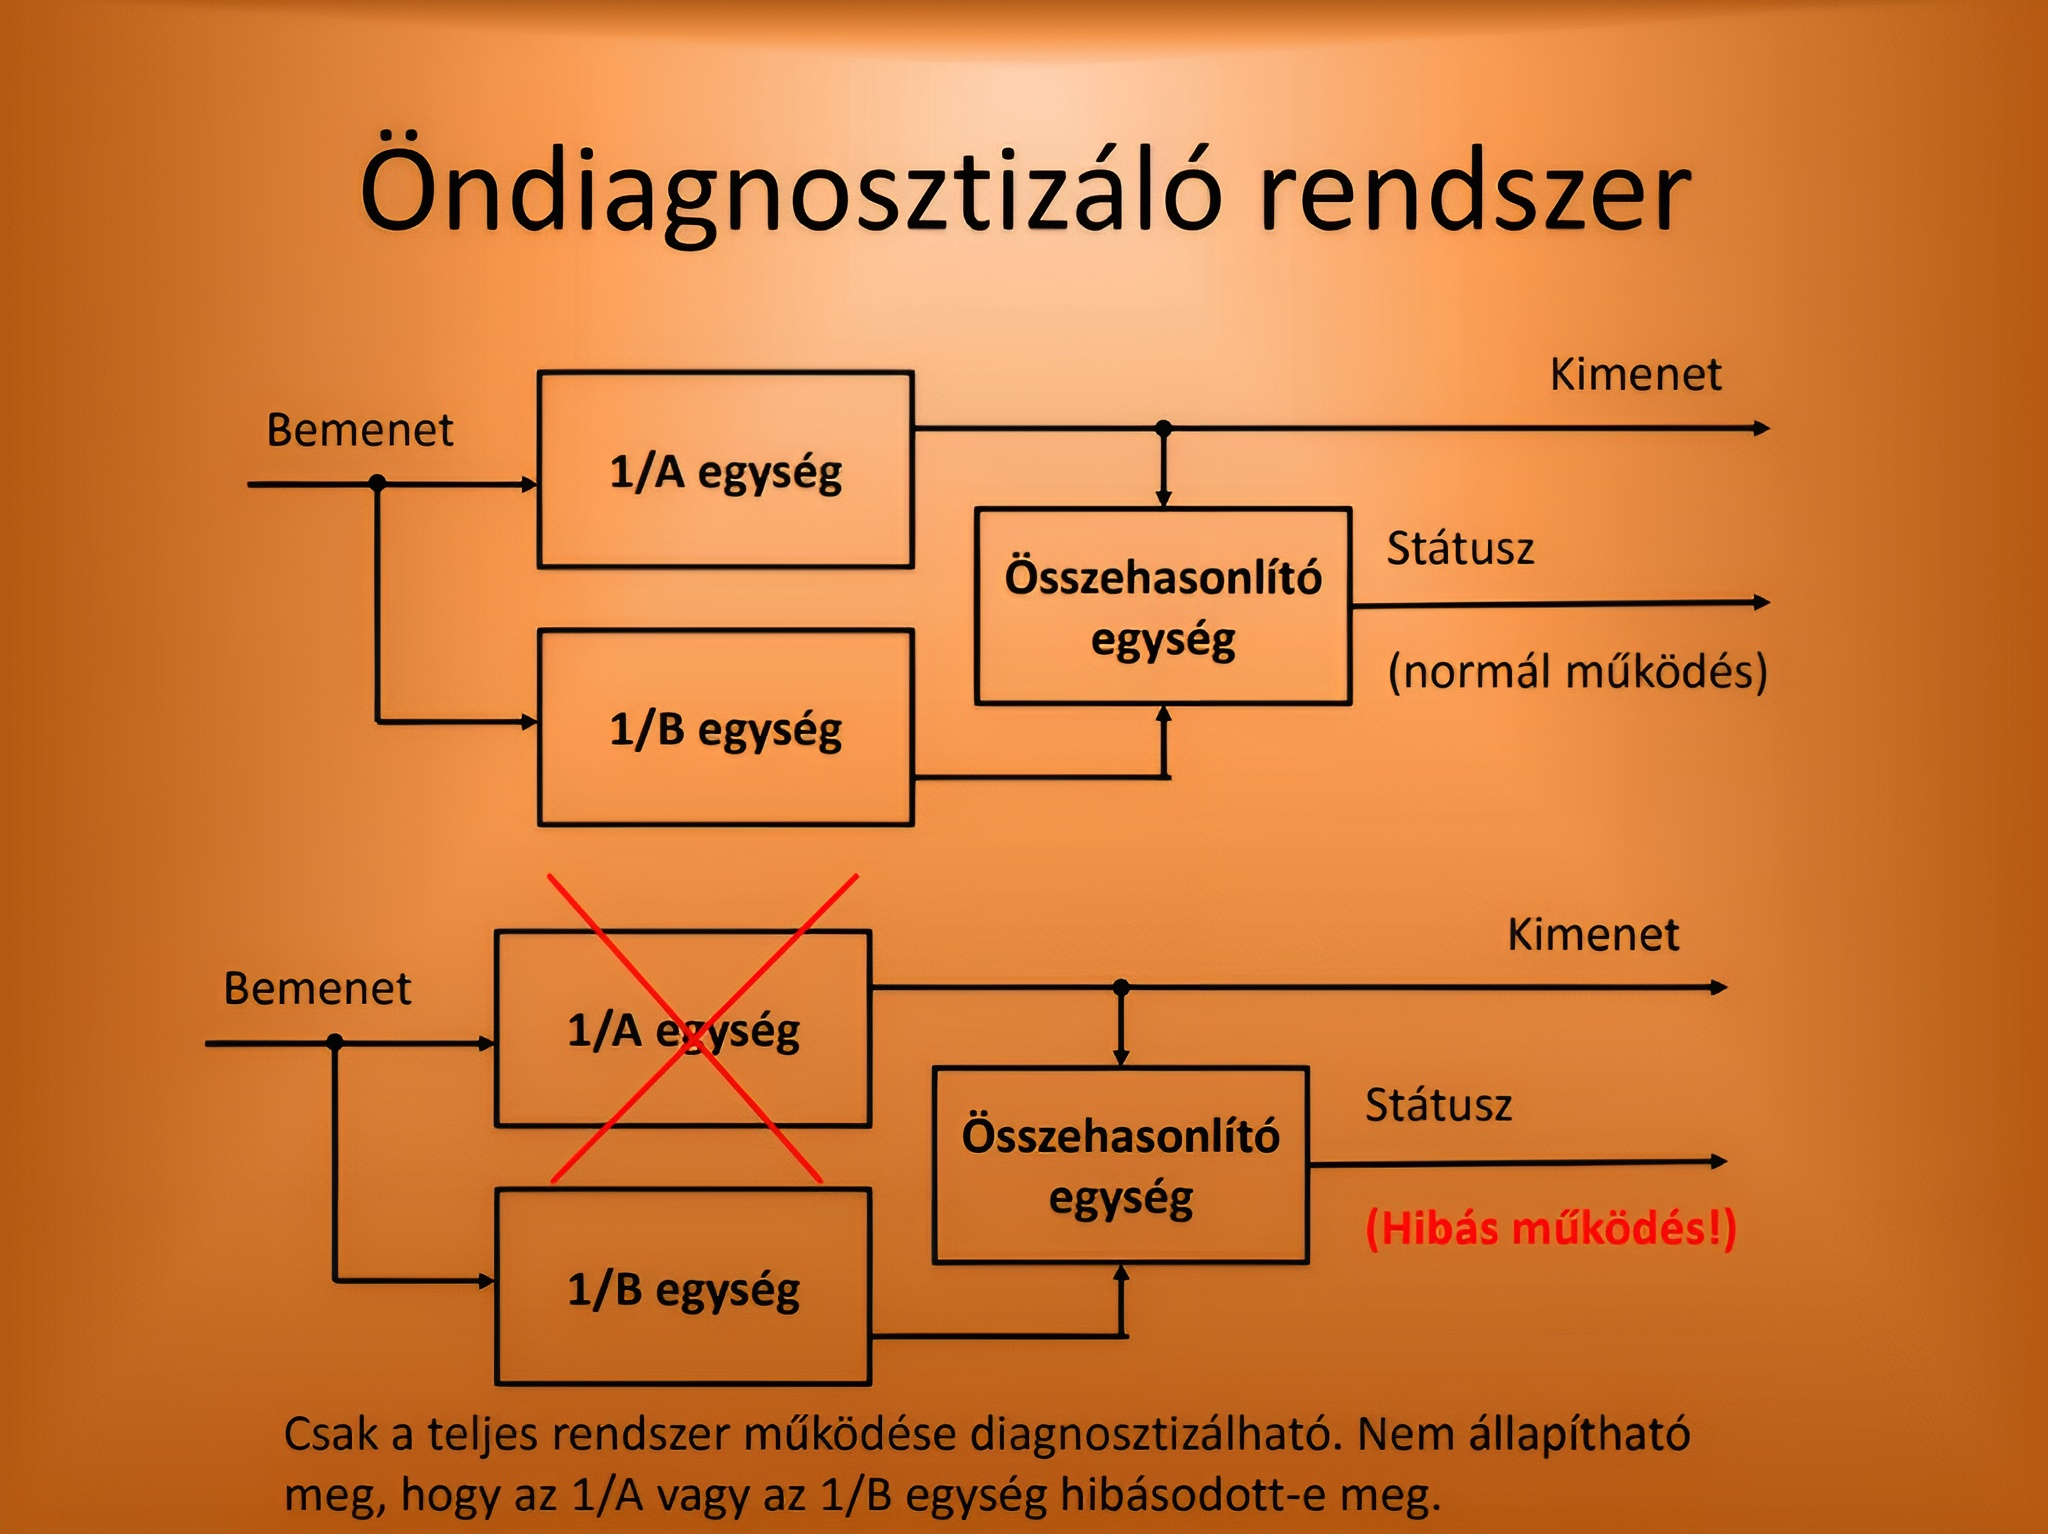
\includegraphics[width=0.7\textwidth]{kep/kep13.png}
    \caption{Öndiagnosztizáló rendszer}
    \label{fig:kep13}
\end{figure}

\begin{figure}[H]
    \centering
    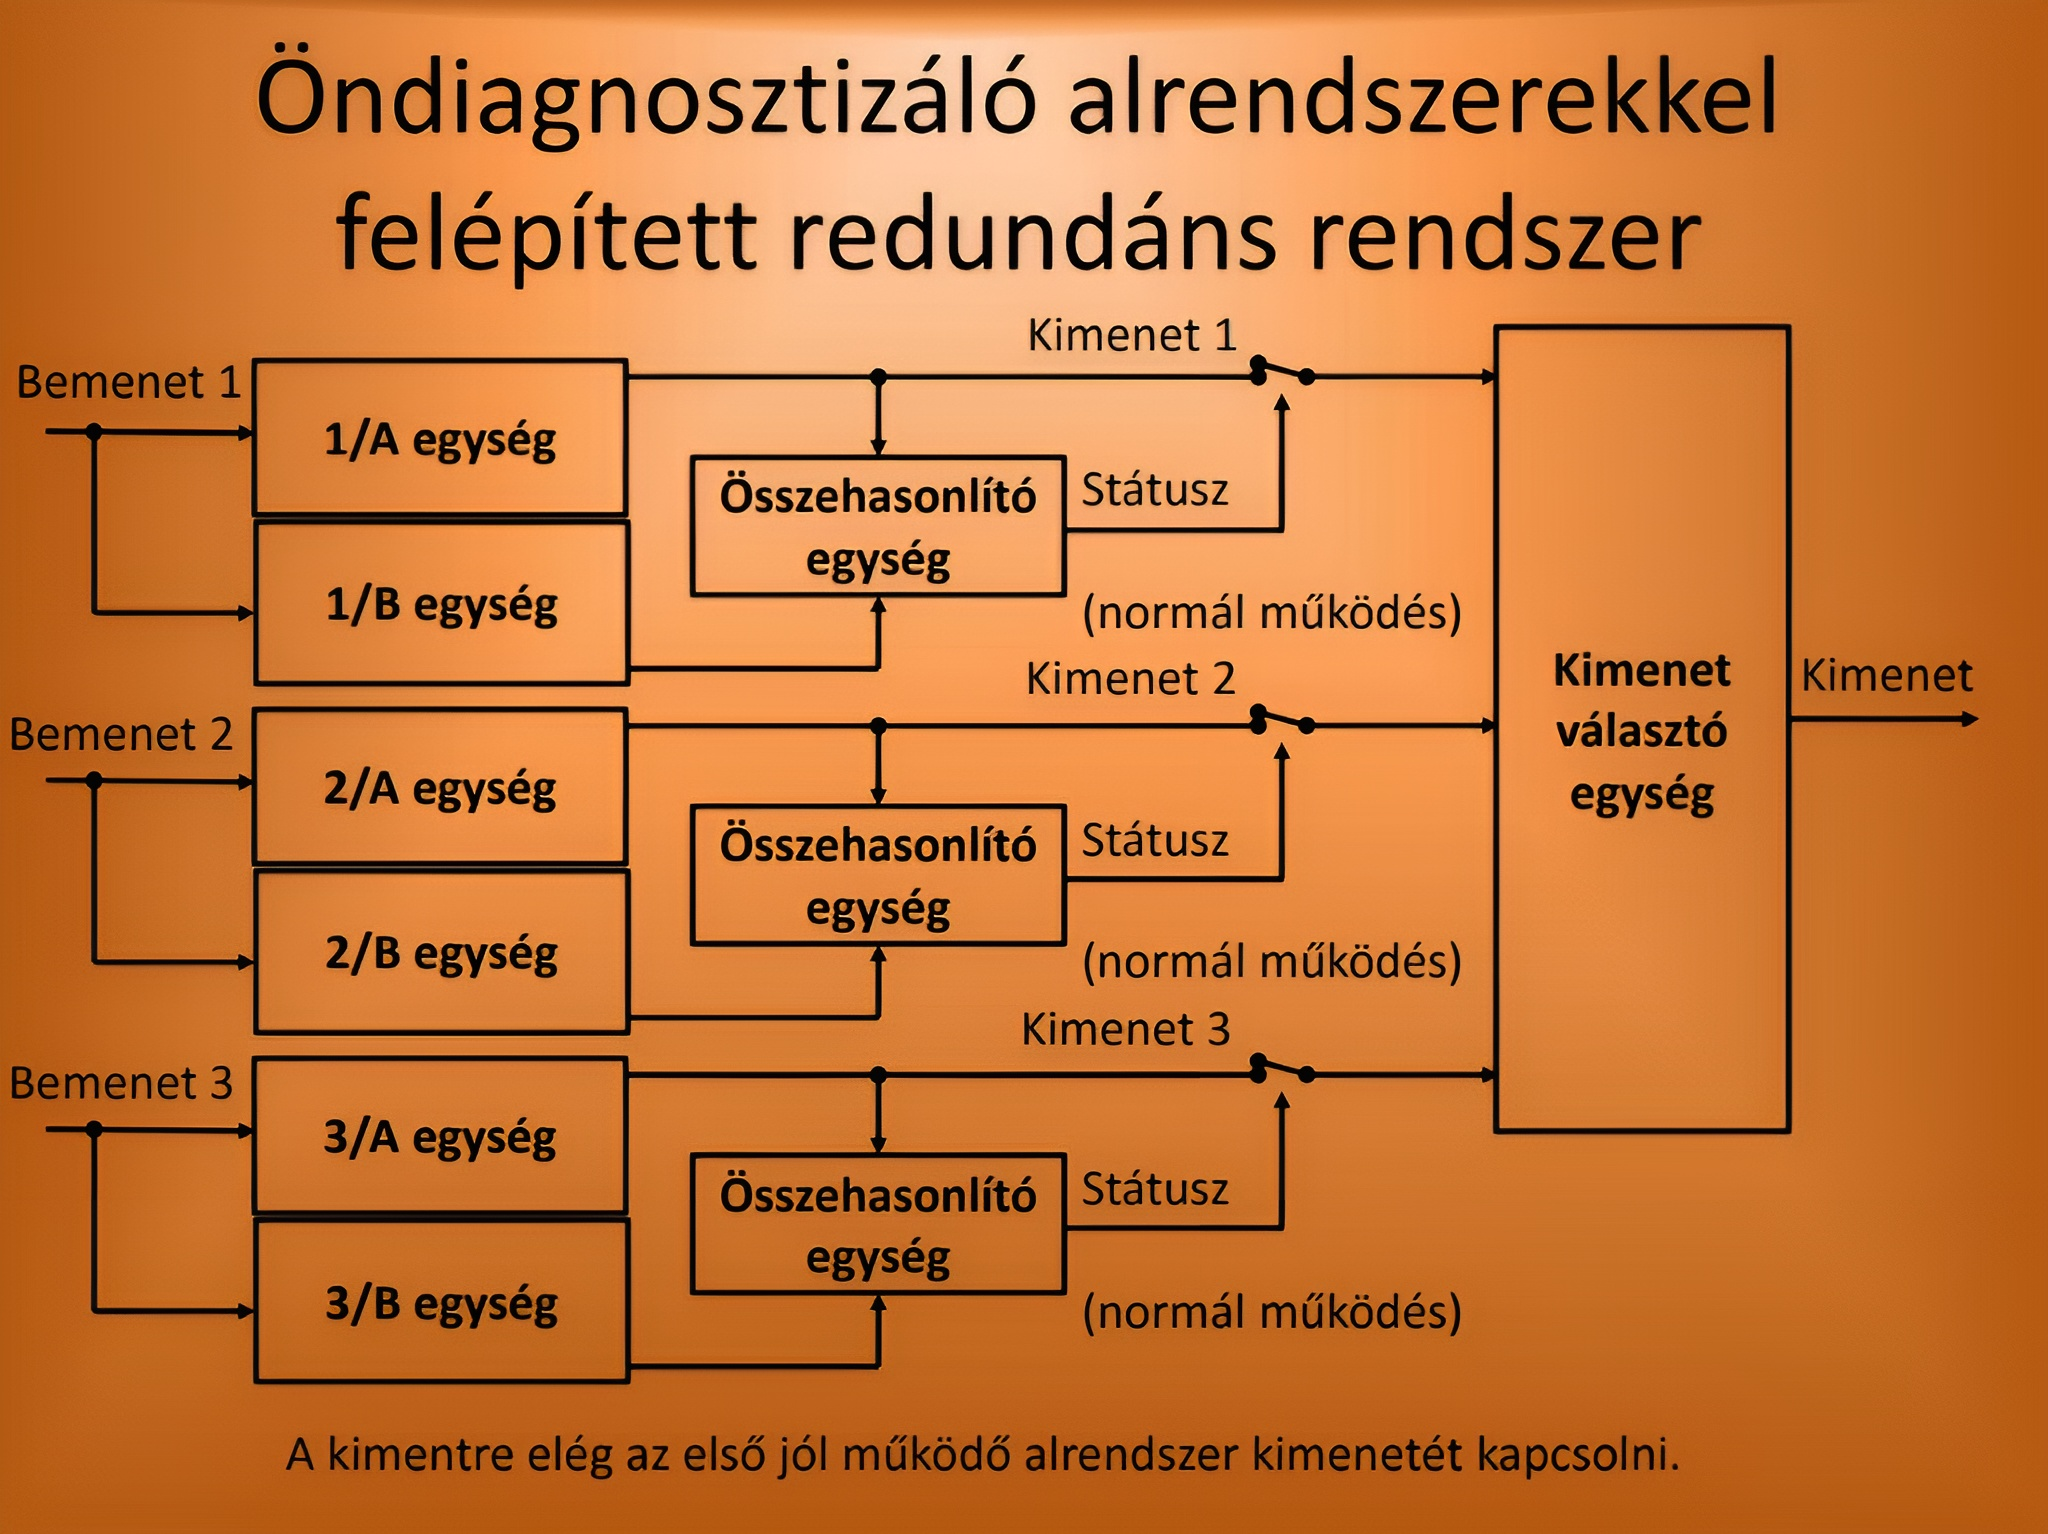
\includegraphics[width=0.7\textwidth]{kep/kep14.png}
    \caption{Öndiagnosztizáló alrendszerekkel felépített redundáns rendeszer normál működése}
    \label{fig:kep14}
\end{figure}

\begin{figure}[H]
    \centering
    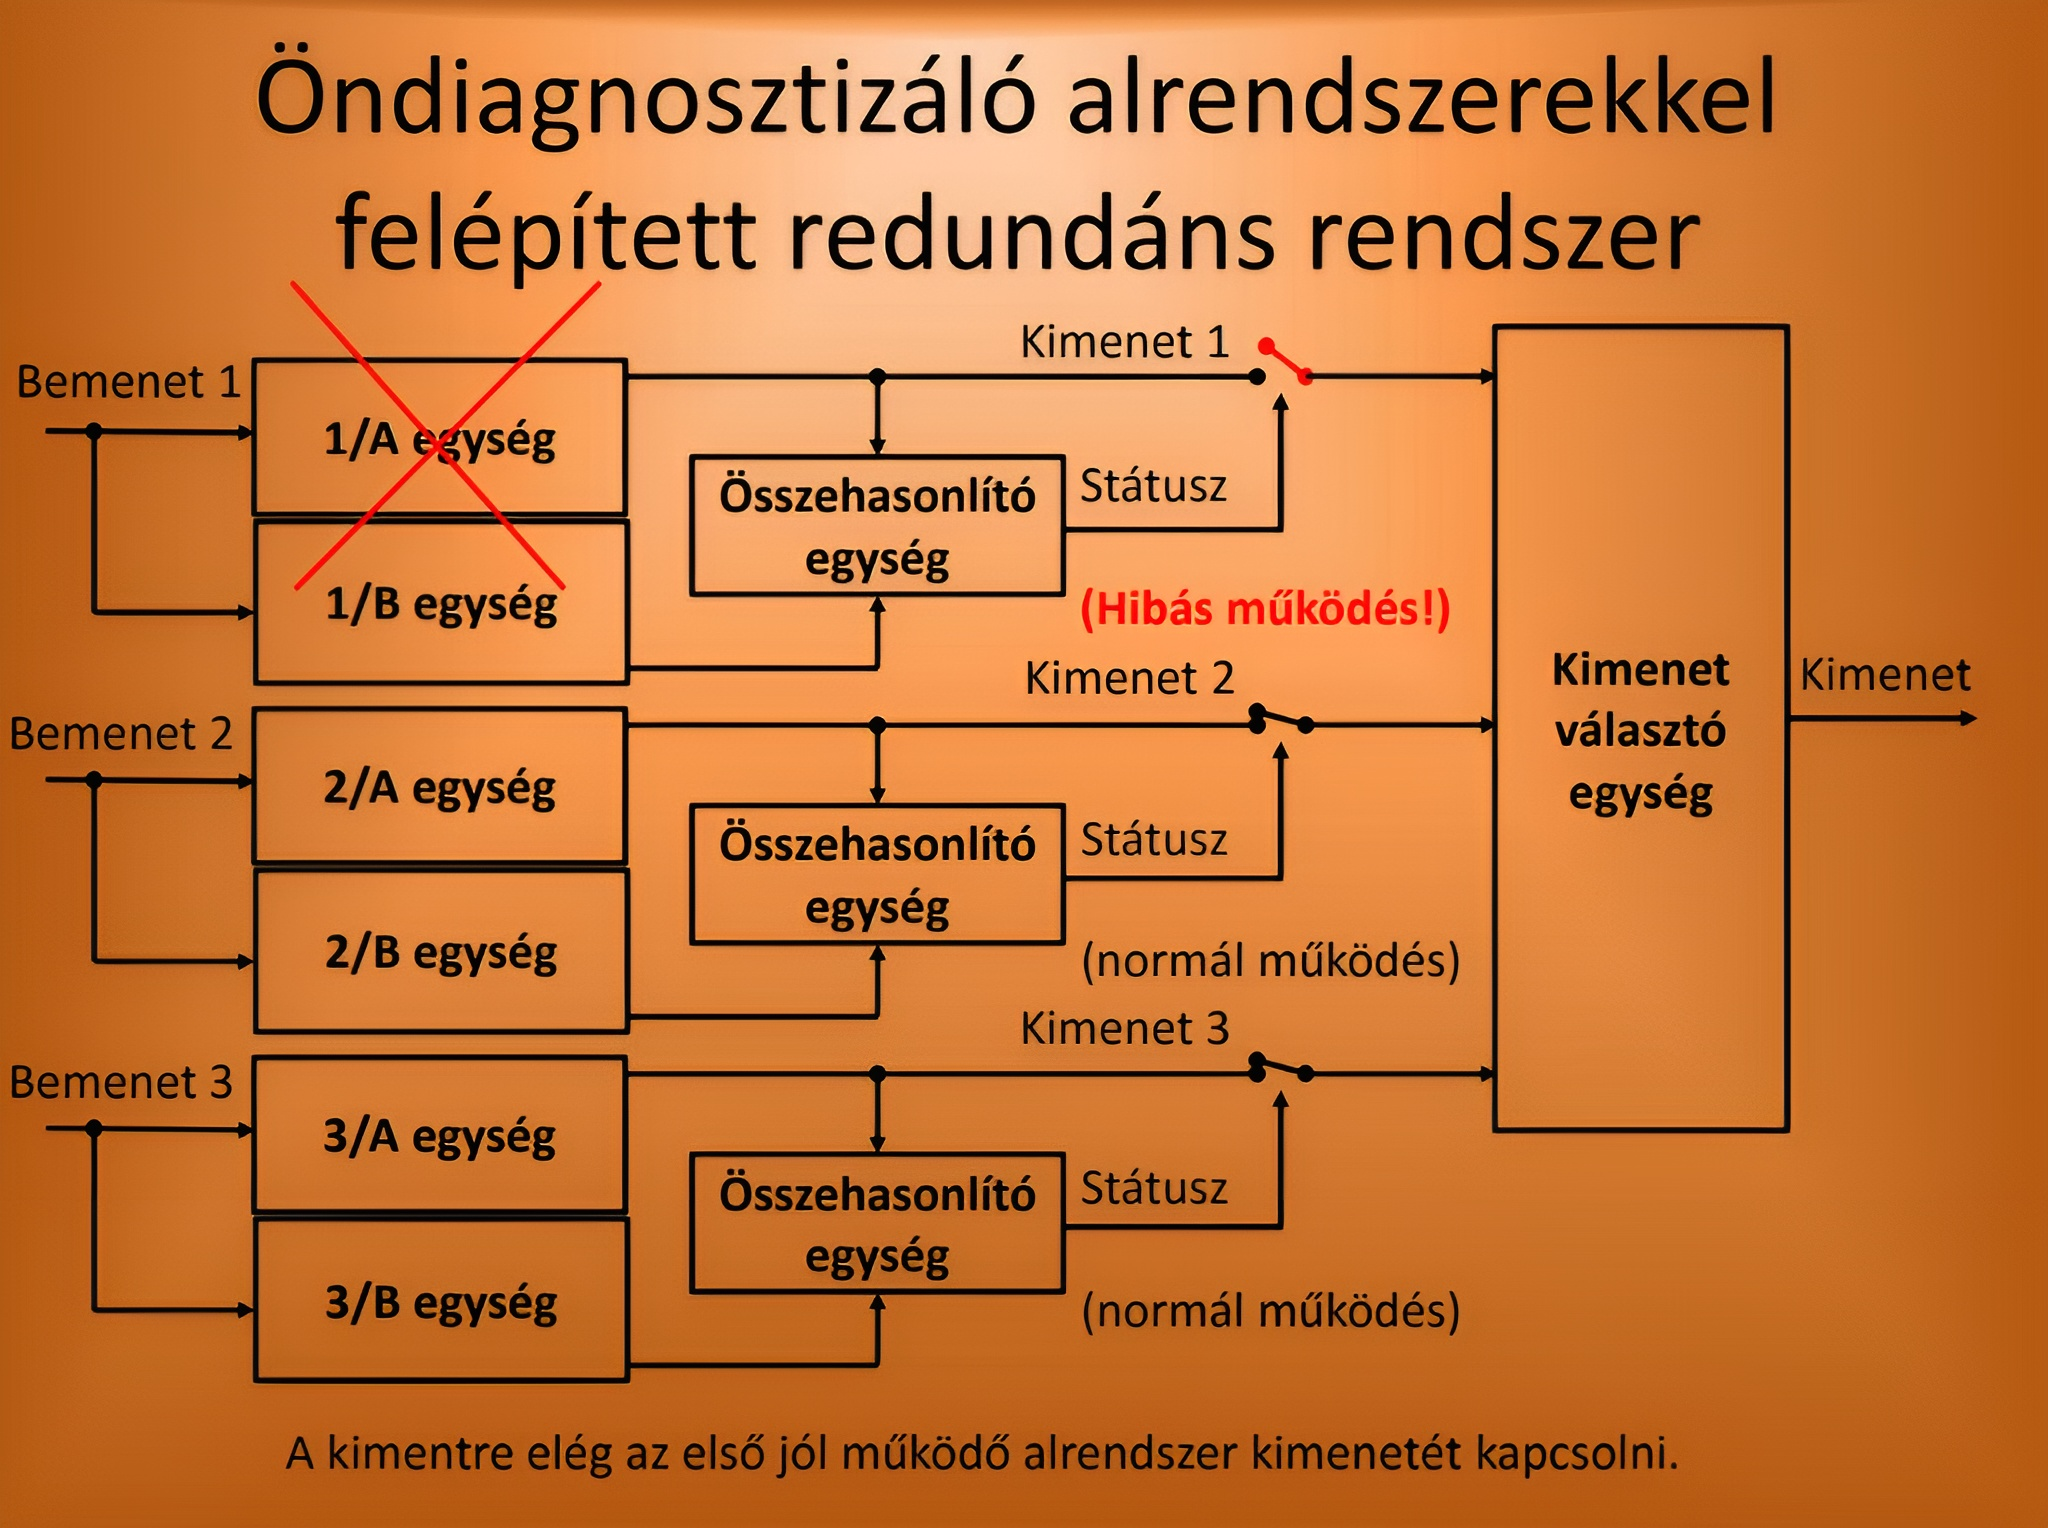
\includegraphics[width=0.7\textwidth]{kep/kep15.png}
    \caption{Öndiagnosztizáló alrendszerekkel felépített redundáns rendeszer hibás működése}
    \label{fig:kep15}
\end{figure}

\begin{itemize}
    \item Összehasonlító egység figyeli az 1/A és 1/B rendszerek működését.
    \item Ugyanez ismételve 2/A és 2/B valamint 3/A és 3/B egységekre.
    \item Végül a kiválasztó egység adja meg az elfogadható kimenetet.
    \item Az önálló egységek a kimenet mellett precizitási kimenetet is adhatnak a kiválasztó áramkör számára.
\end{itemize}

\section{Minőségi jellemzőkön alapuló redundáns rendszer}

\begin{figure}[H]
    \centering
    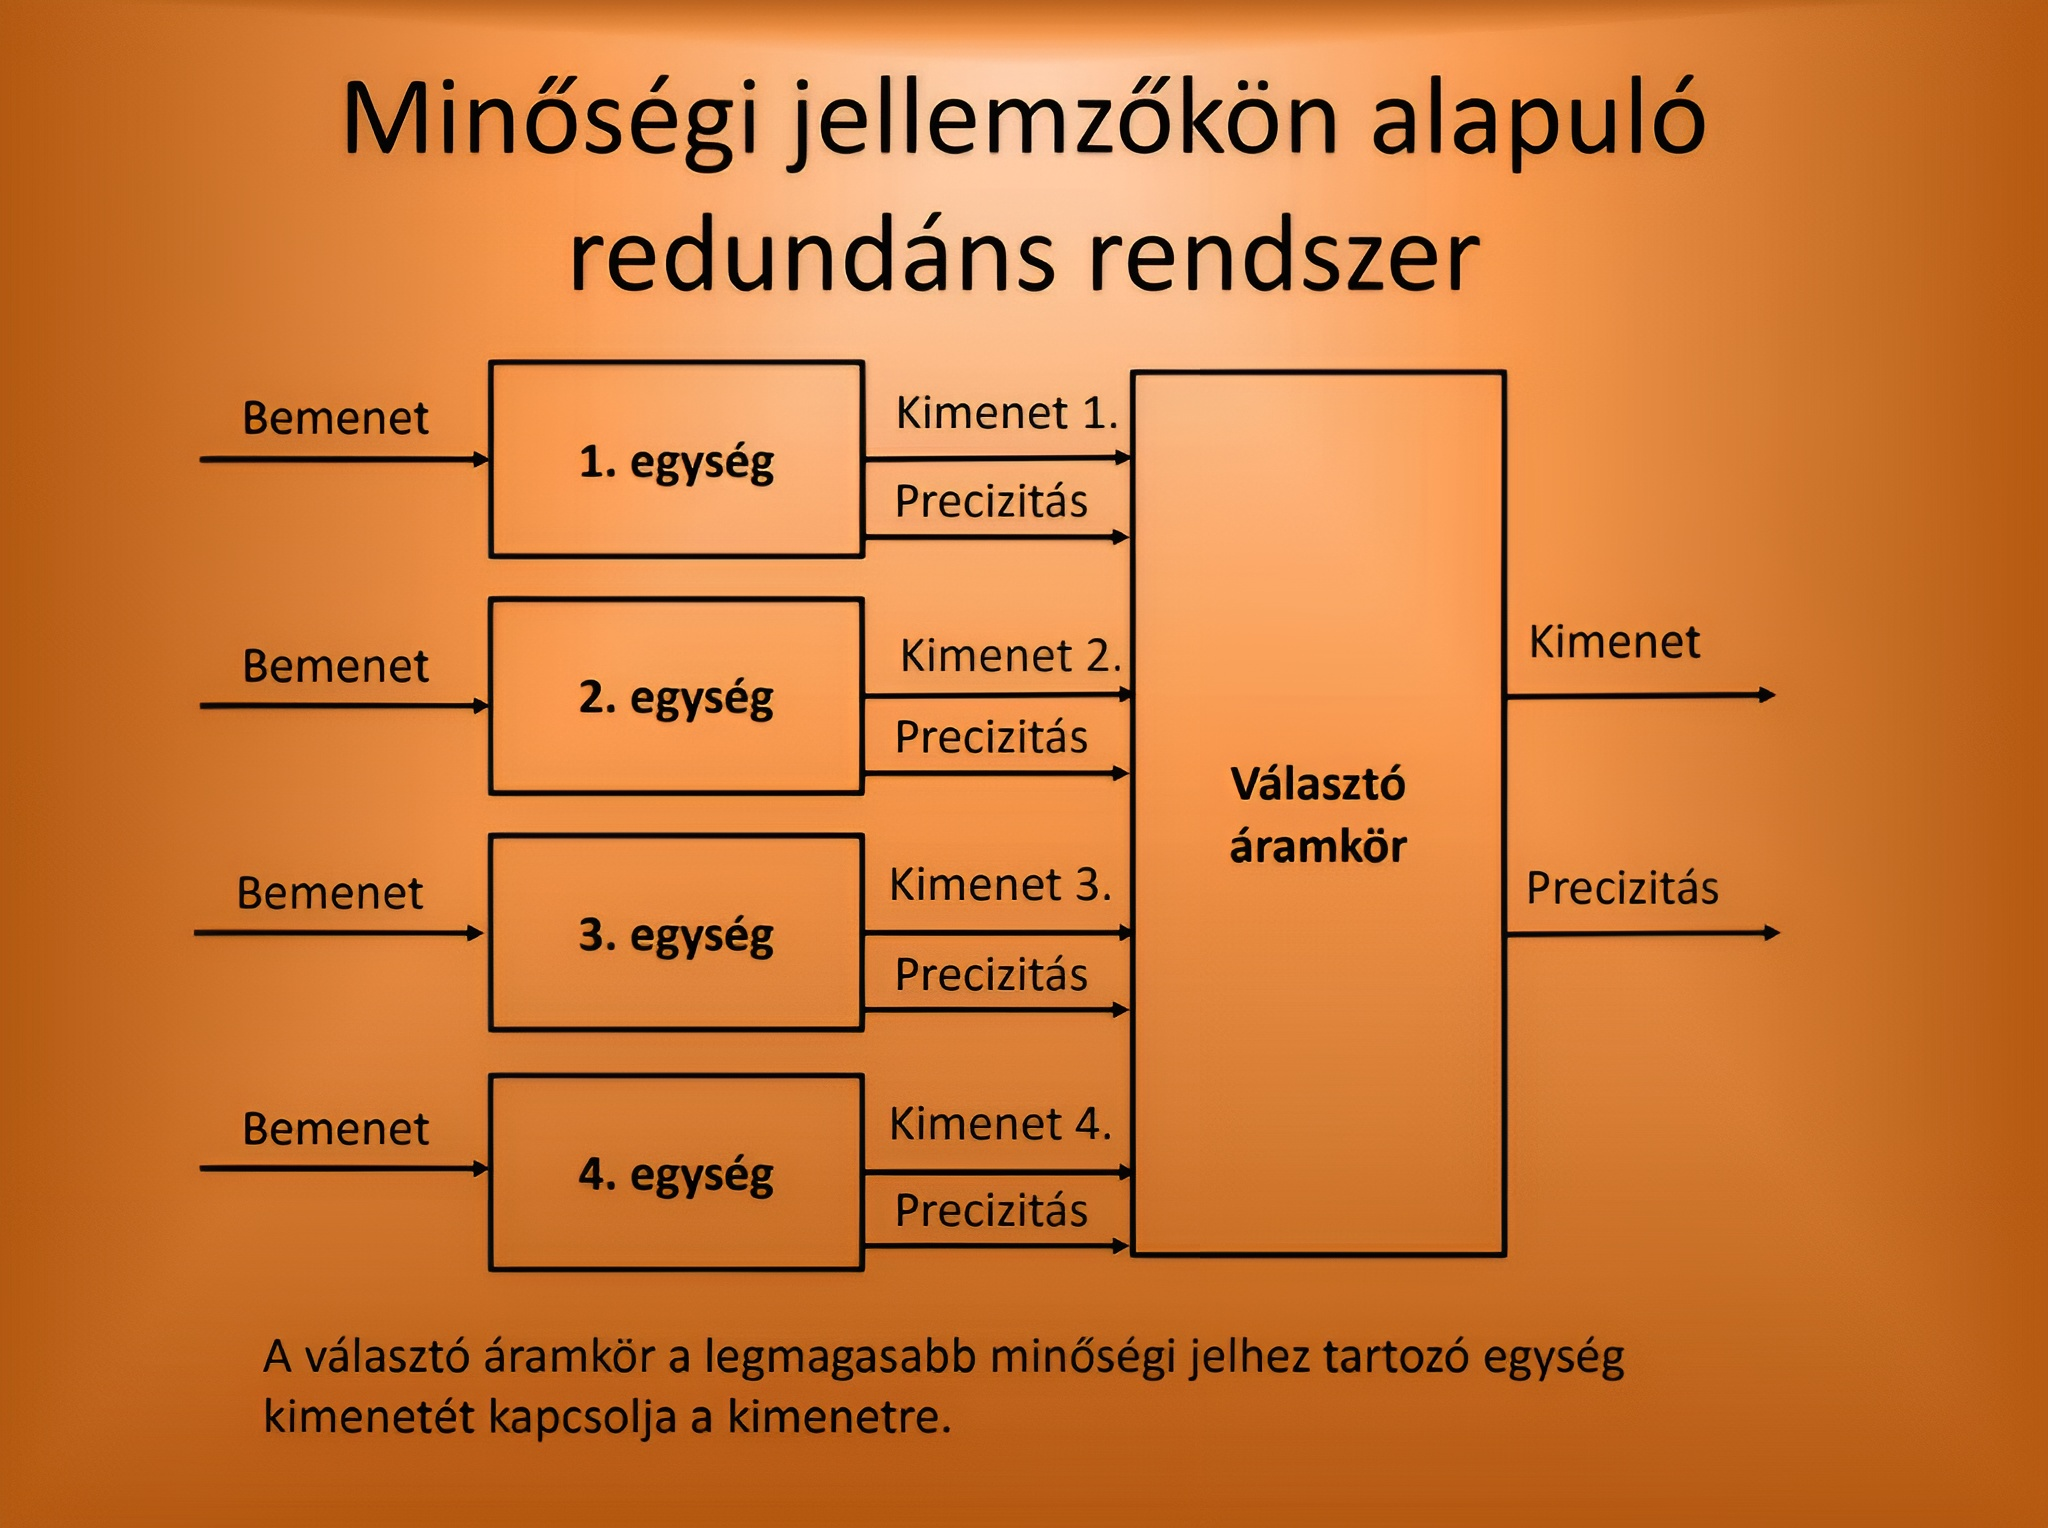
\includegraphics[width=0.7\textwidth]{kep/kep16.png}
    \caption{Minőségi jellemzőkön alapuló redundáns rendszer}
    \label{fig:kep16}
\end{figure}

\begin{figure}[H]
    \centering
    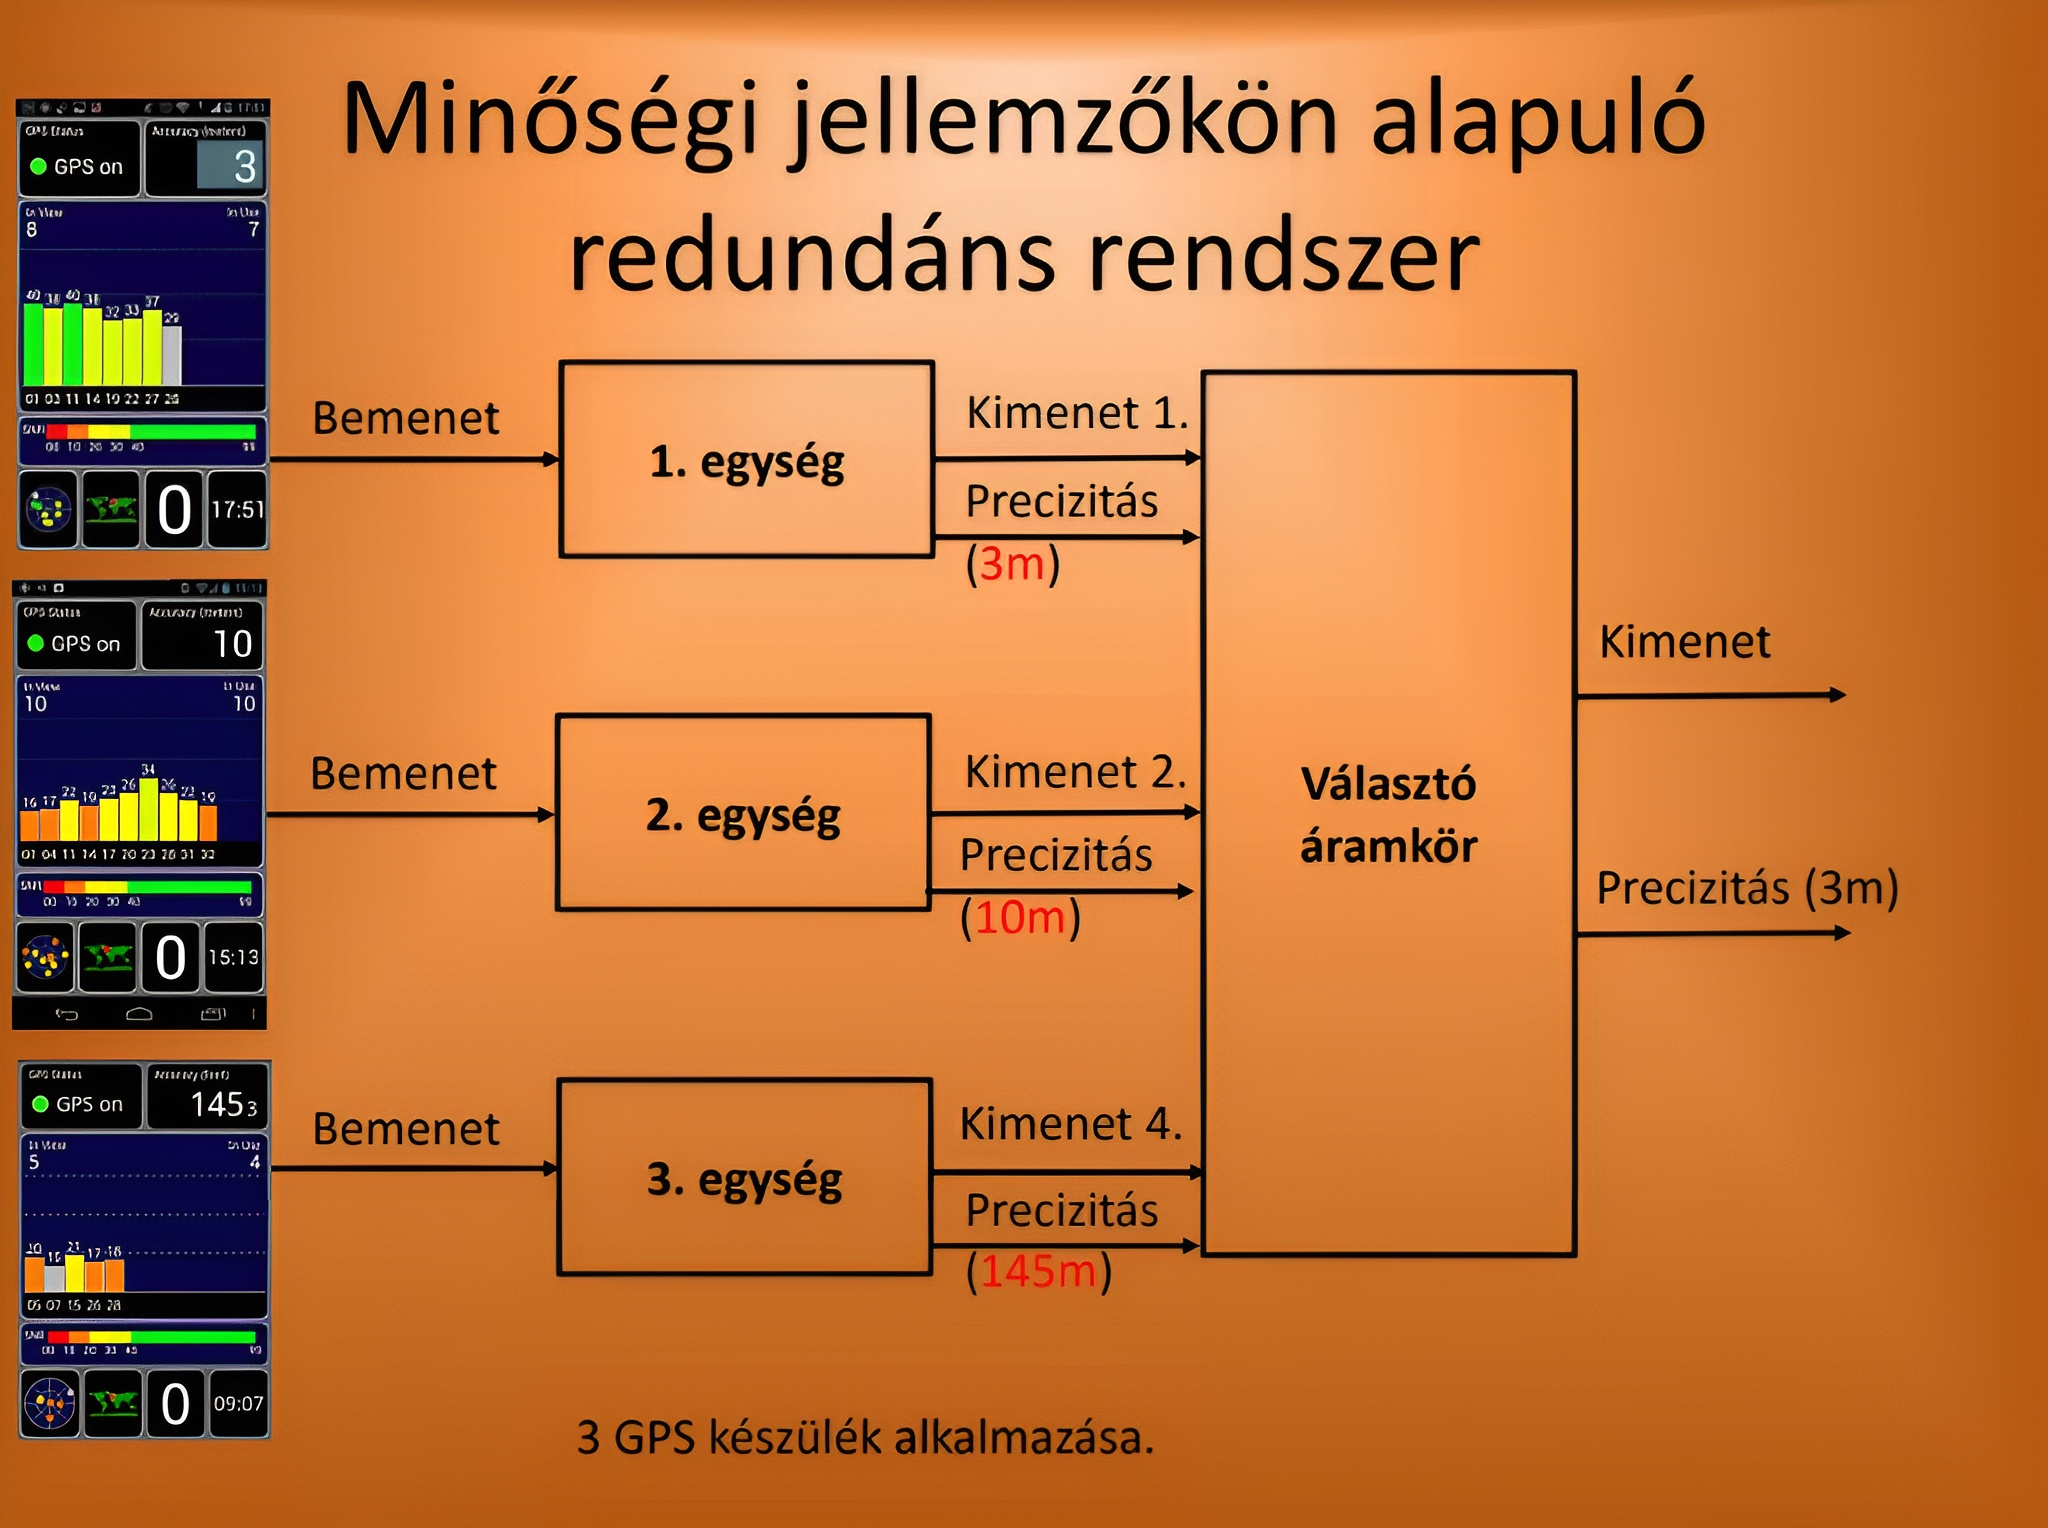
\includegraphics[width=0.7\textwidth]{kep/kep17.png}
    \caption{Minőségi jellemzőkön alapuló redundáns rendszer működése}
    \label{fig:kep17}
\end{figure}

\begin{itemize}
    \item A választó áramkör a legmagasabb minőségi jelhez tartozó egység kimenetét kapcsolja a kimenetre.
    \item A választó áramkör a kimeneti jel mellett egy precizitás jelet is kap minden egységtől.
    \item A teljes rendszer eredménye a normál kimenet lesz és a hozzá tartozó precizitás jel.
\end{itemize}

\section{Hibrid redundáns HW rendszer}

\subsection{Teljes értékű egység és Minimál felügyeleti egység között belső kommunikáció}

\begin{itemize}
    \item A komplex fő egység meghibásodásának valószínűsége nagyobb, mint az egyszerűbb felépítésű ellenőrző egységé.
    \item Az ellenőrző egység egyben biztosítja a teljes rendszer minimális szolgáltatási szintjét.
    \item A választó áramkör értesül, hogy az egyik egység meghibásodott, így vagy csak a fő egység, vagy csak a tartalék egység fog működni.
    \item Tehát ha a \textbf{teljes értékű egység} meghibásodik, a \textbf{minimál felügyeleti egység} teljeskörű adatot fog biztosítani, de \textbf{tájékoztat a státusz vezetéken keresztül, hogy csökkentett módban működik}.
\end{itemize}

\begin{figure}[H]
    \centering
    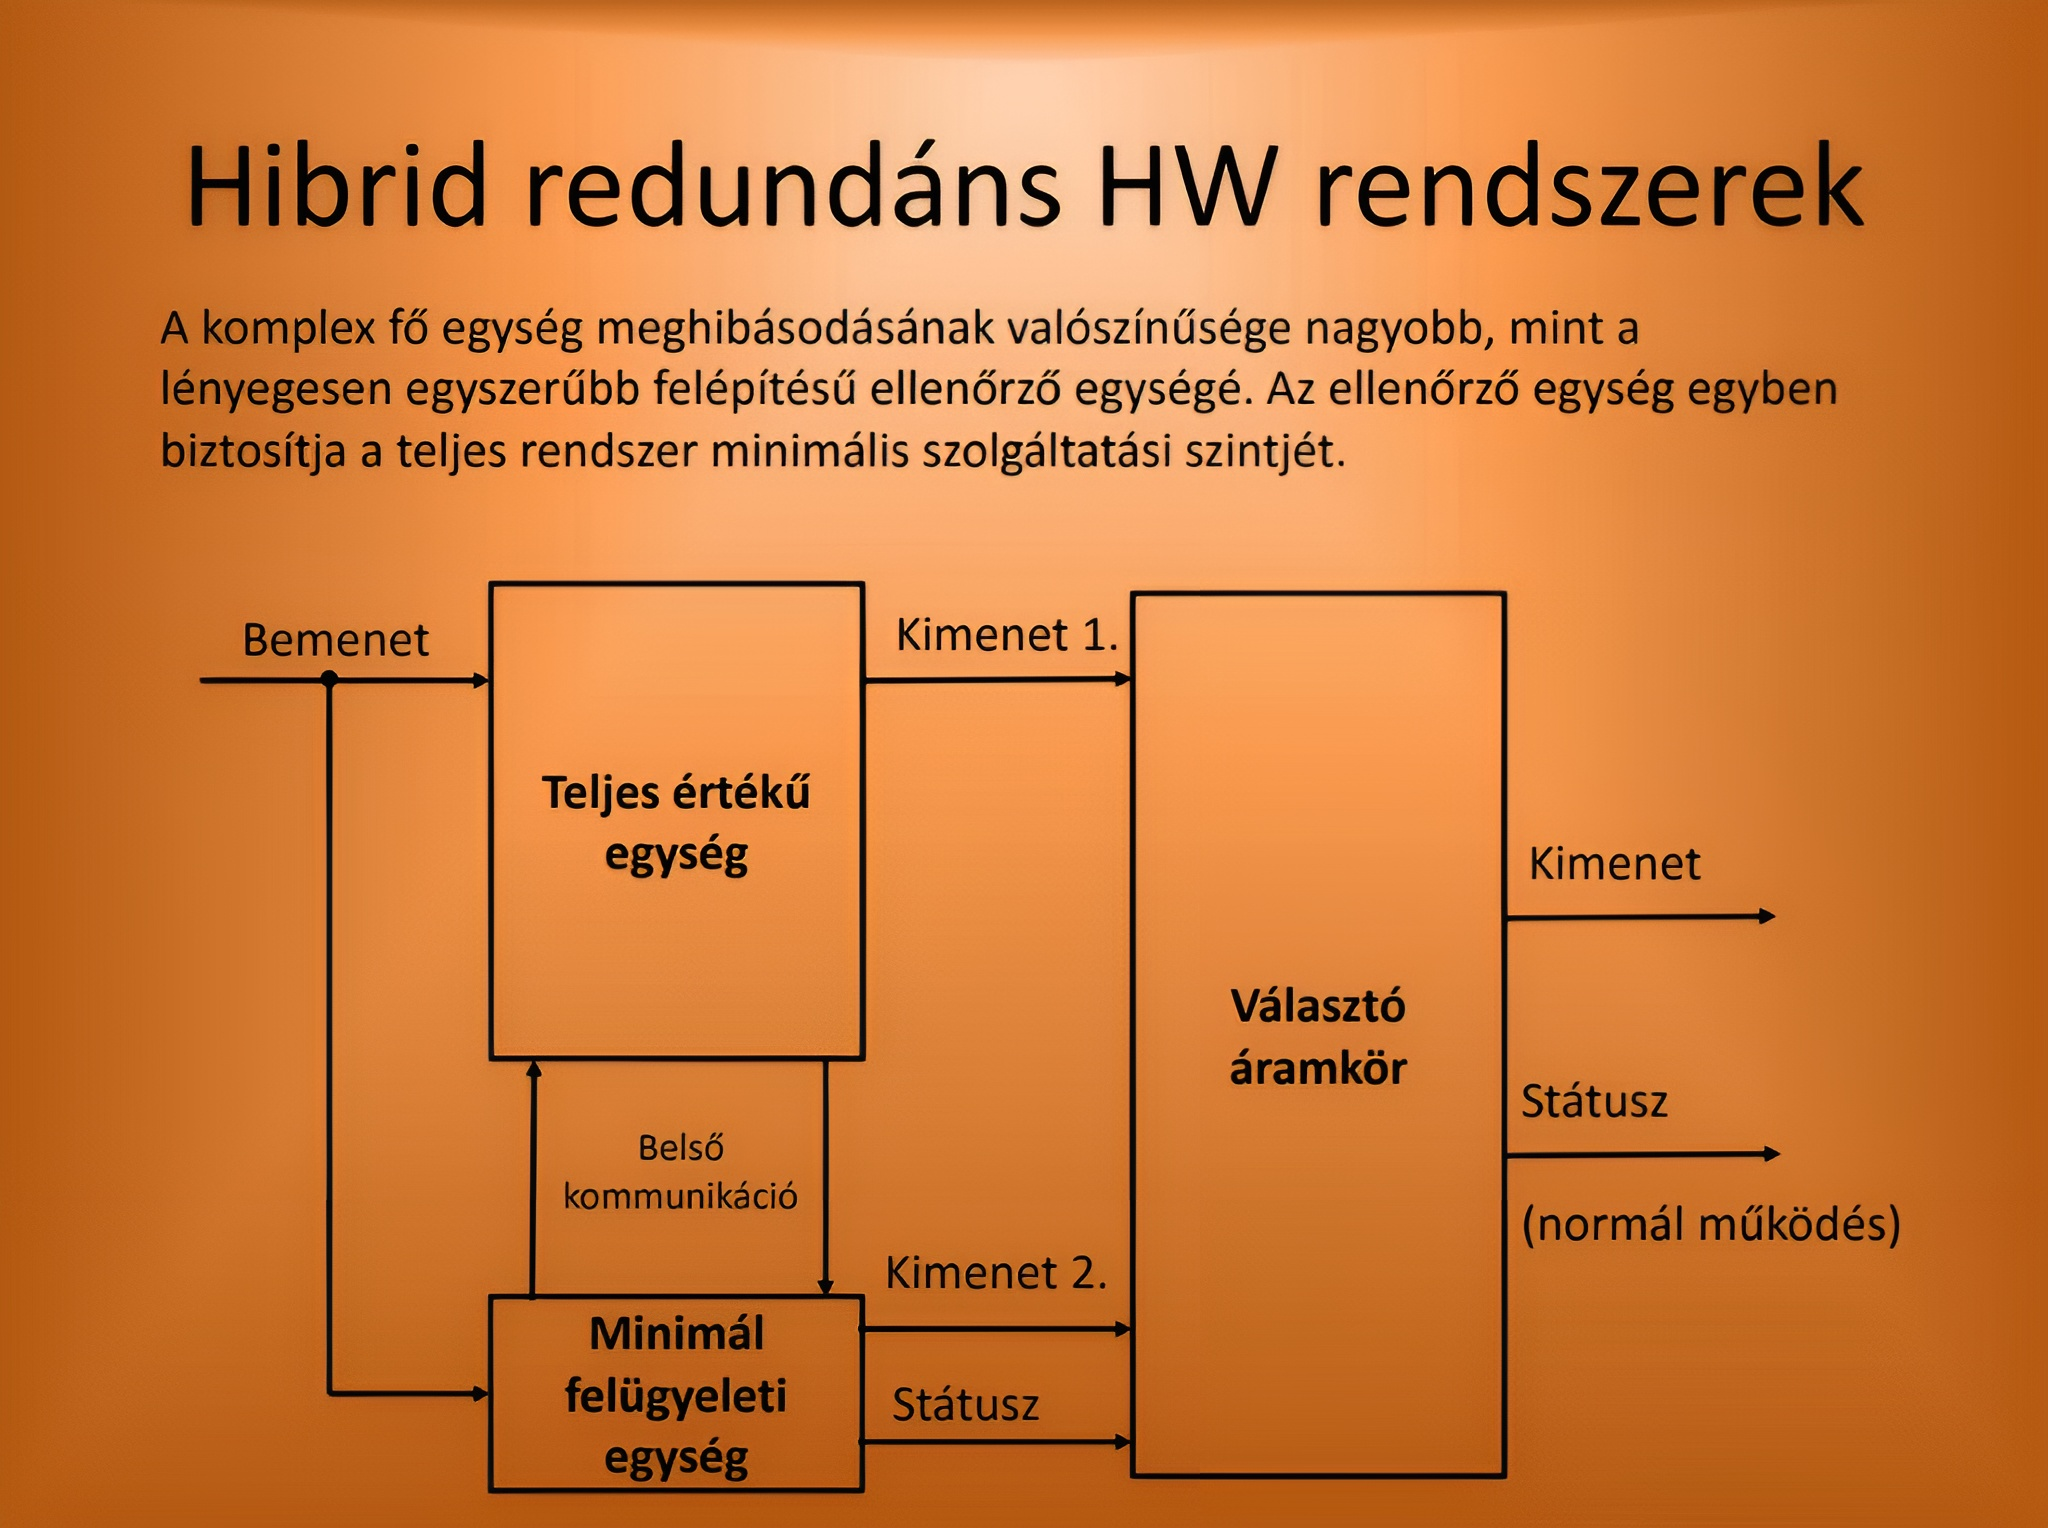
\includegraphics[width=0.7\textwidth]{kep/kep18.png}
    \caption{Hibrid redundáns HW rendszer működése}
    \label{fig:kep18}
\end{figure}

\subsection{Watchdog}
\begin{itemize}
    \item \textbf{WD = Watchdog, életjel figyelő áramkör:} időnként ellenőrzi, hogy a főprogram ciklusa helyesen lefutott-e.
    \item Amennyiben a fő ciklus nem fut le, és nem történik életjel visszajelzés, a \textbf{Watchdog reset jelet küld,} és újraindítja a fő processzort.
    \item A Mikrovezérlő része a Watchdog timer.
    \item Fejlesztéskor nem szabad bekapcsolni, mert nem lehetne szüneteltetni a kód futását debug céljából, mivel újraindítaná a processzort.
    \item A fejlesztés végén \textbf{meg kell határozni a ciklusidőt, beállítani a watchdog számára,} és engedélyezni a működését.
\end{itemize}

\begin{figure}[H]
    \centering
    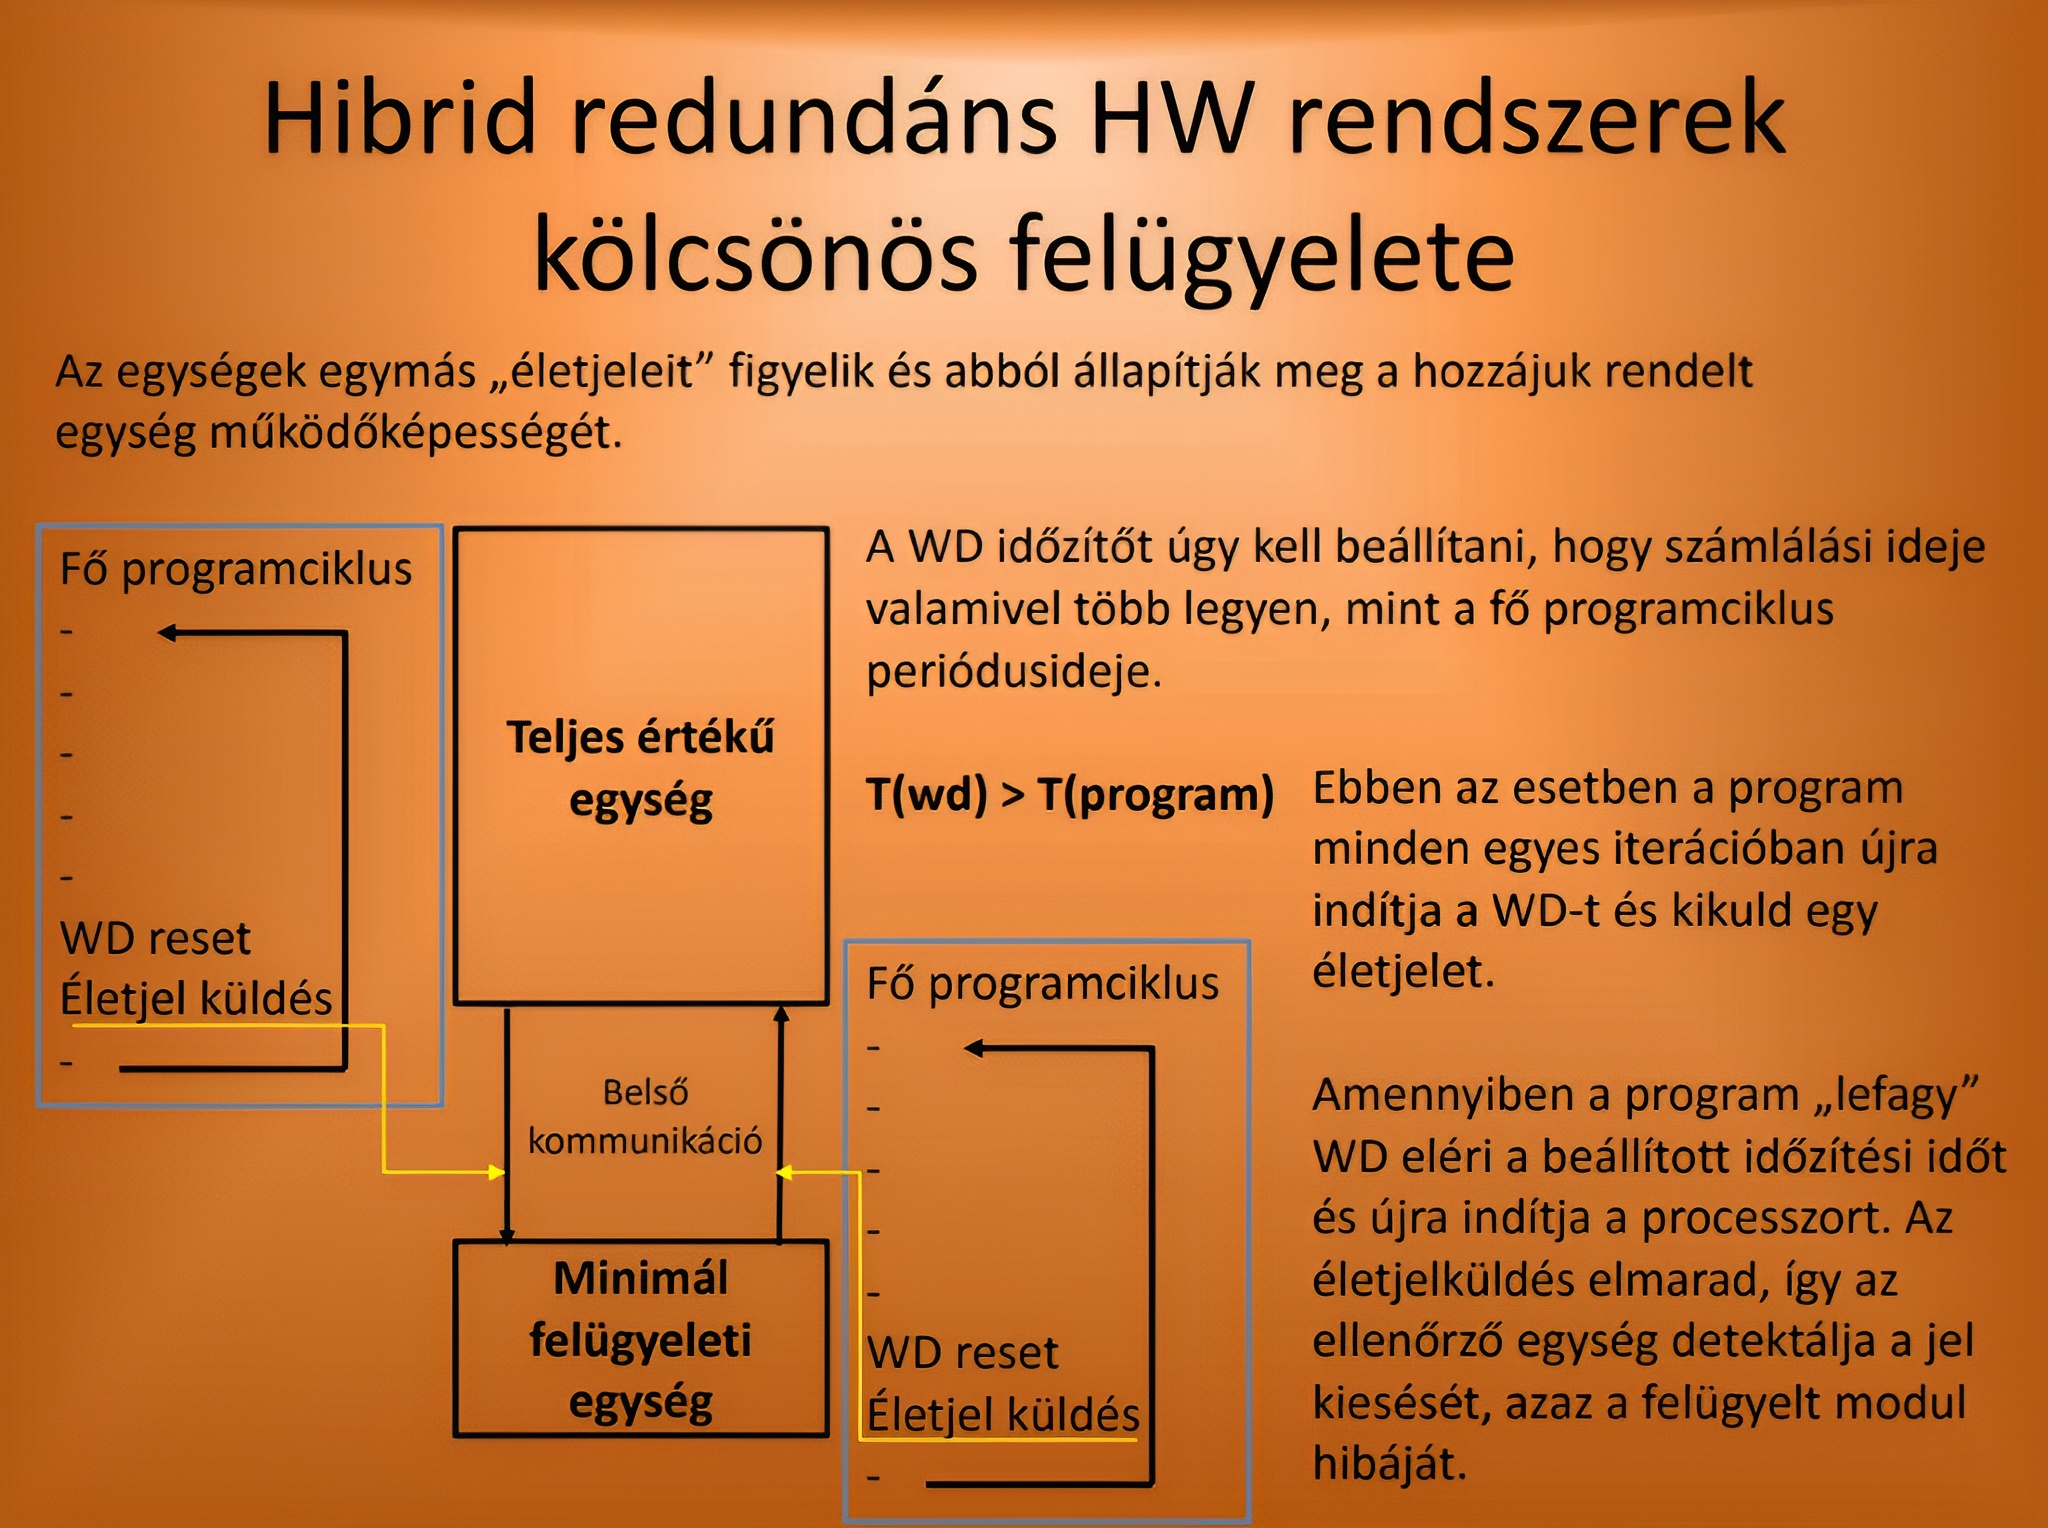
\includegraphics[width=0.7\textwidth]{kep/kep19.png}
    \caption{Hibrid redundáns HW rendszer felügyelete}
    \label{fig:kep19}
\end{figure}

\begin{figure}[H]
    \centering
    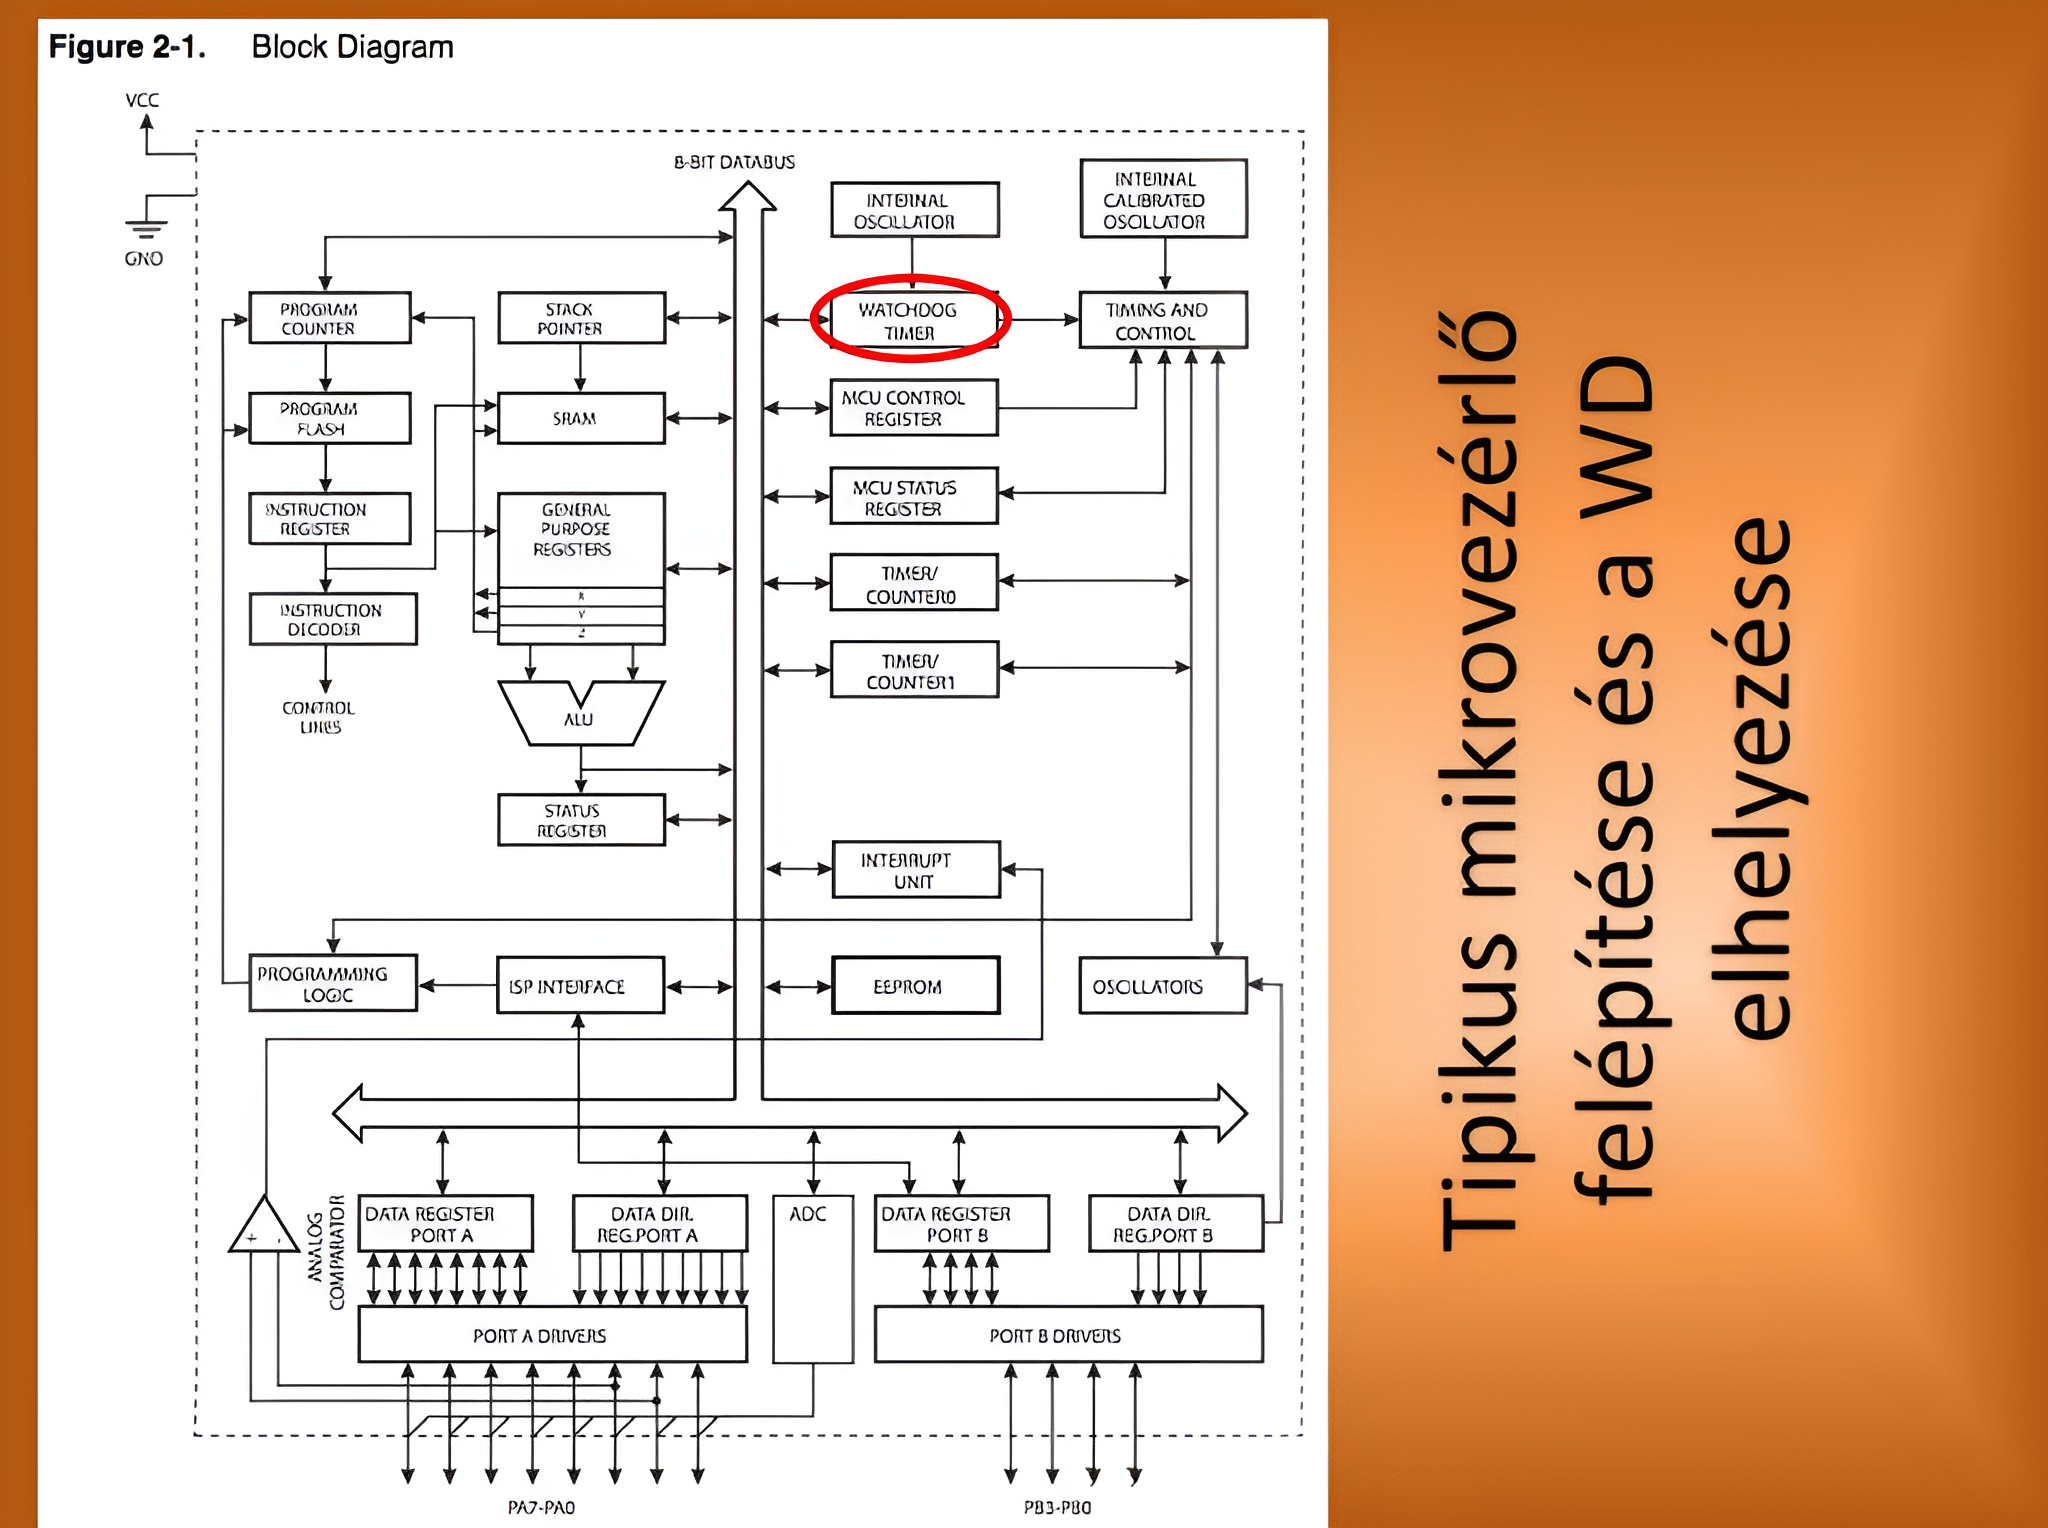
\includegraphics[width=0.7\textwidth]{kep/kep20.png}
    \caption{Hibrid redundáns HW rendszer - Watchdog}
    \label{fig:kep20}
\end{figure}

\section{A termék életciklusa}

\subsection{A meghibásodás valószínűsége}

\begin{itemize}
    \item A meghibásodás valószínűsége az eszköz korával nő, eleinte kevésbé valószínű, majd növekszik.
    \item A rendelkezésreállást ugyanígy vázolhatjuk, csak a meghibásodás inverzével.
\end{itemize}

\begin{figure}[H]
    \centering
    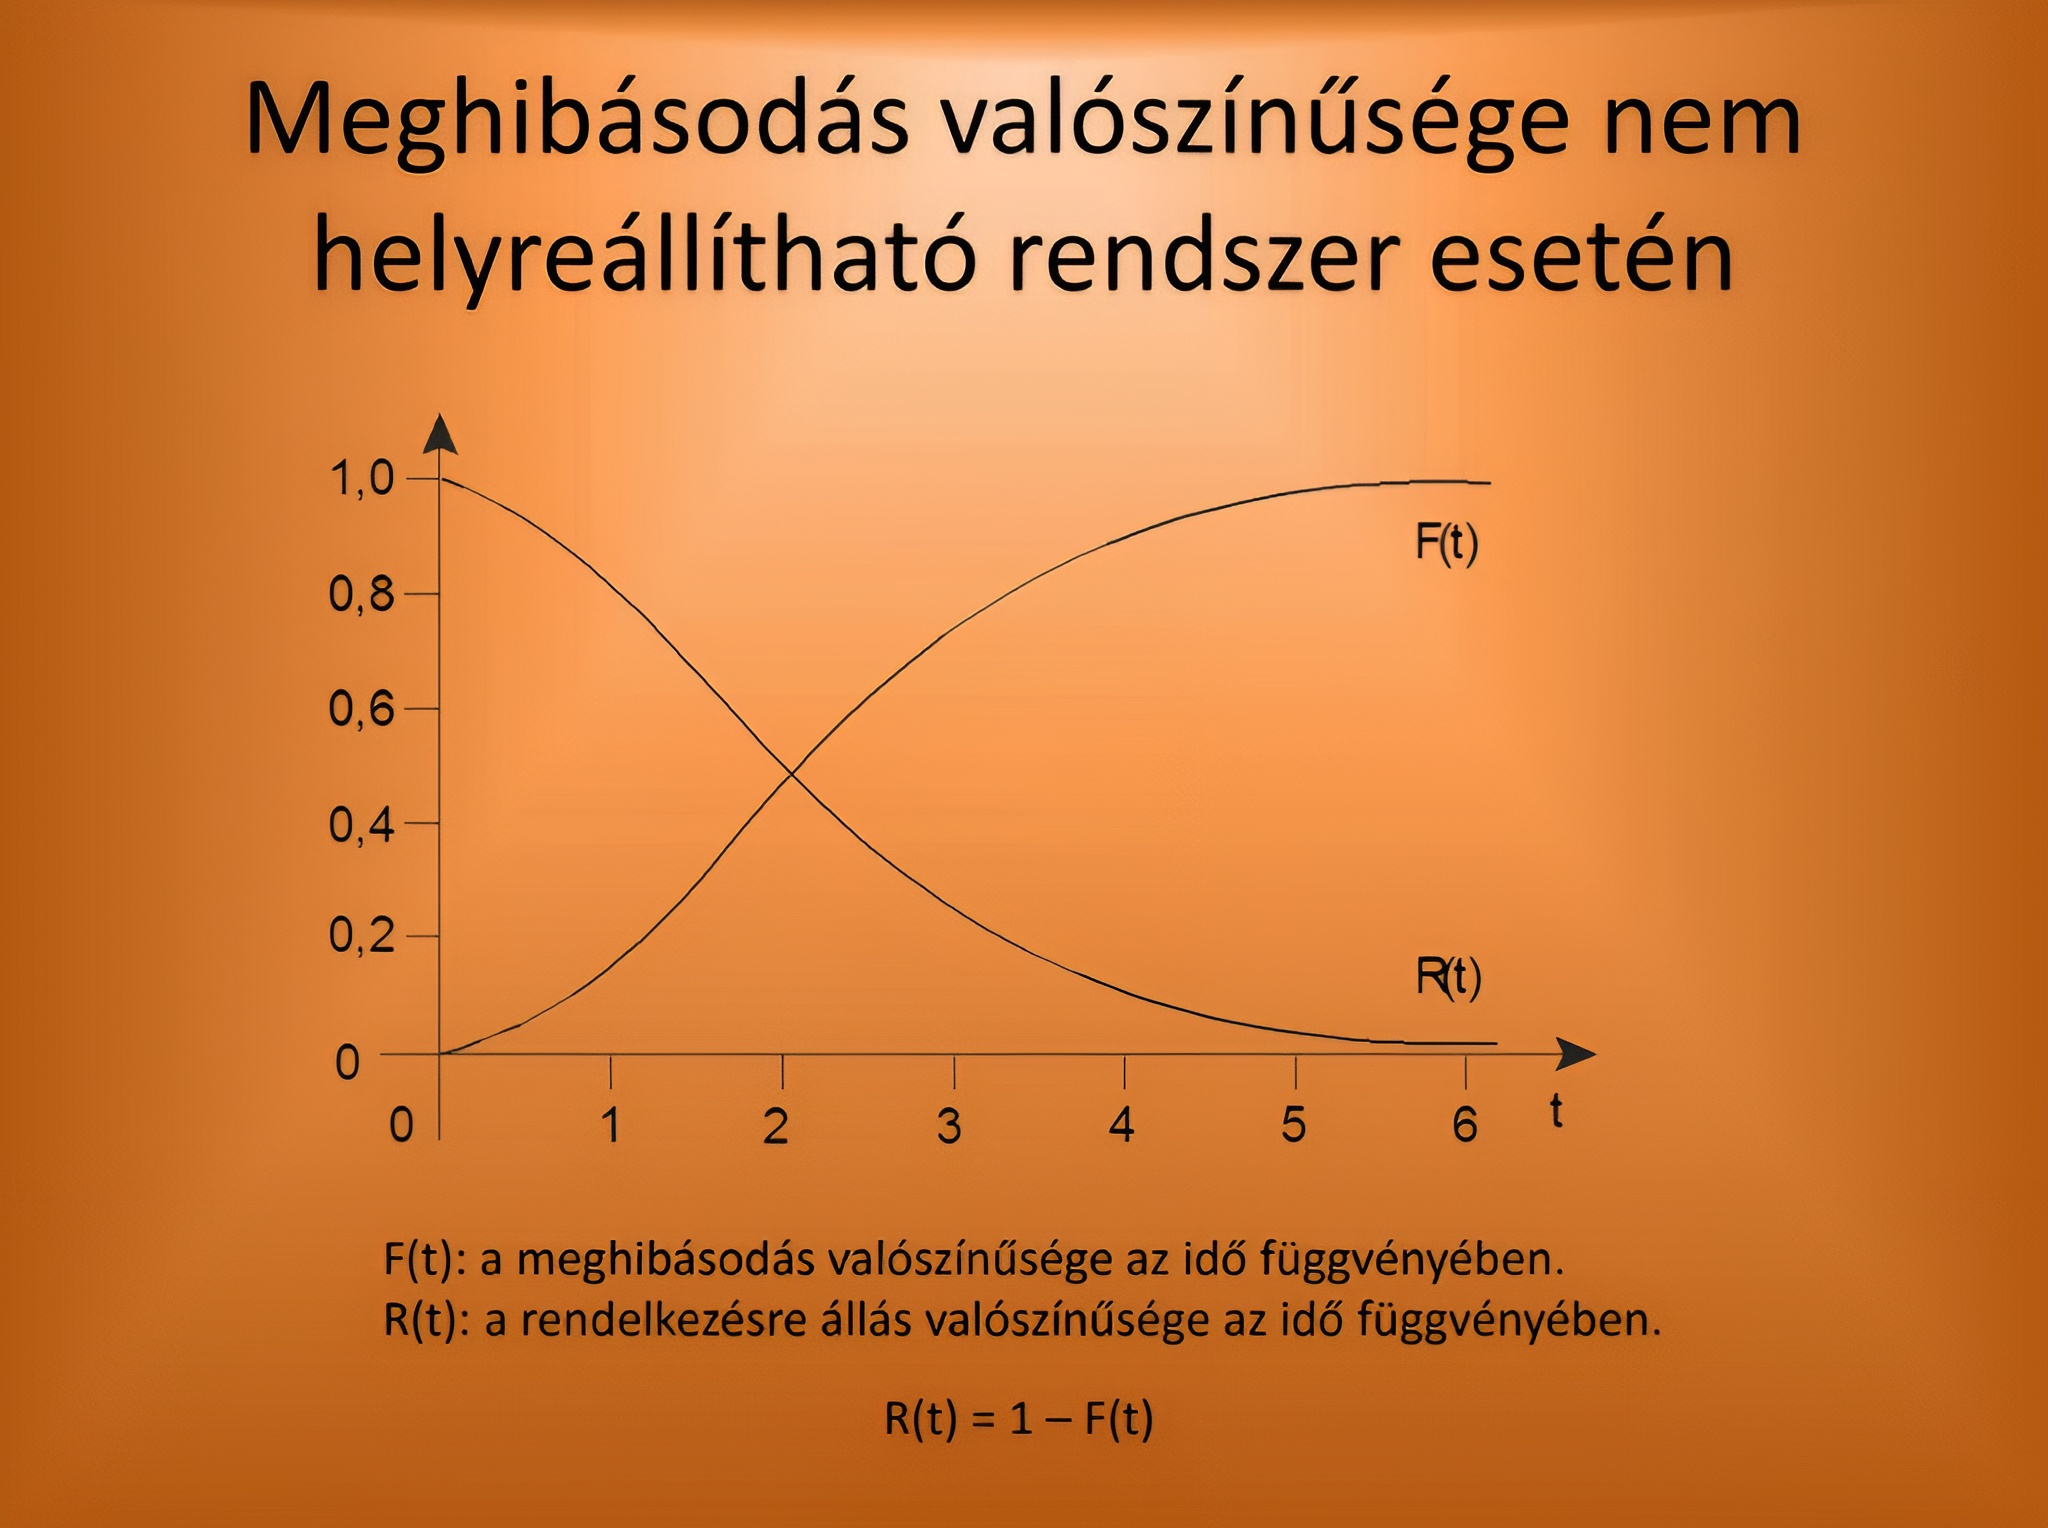
\includegraphics[width=0.7\textwidth]{kep/kep21.png}
    \caption{Meghibásodás valószínűsége}
    \label{fig:kep21}
\end{figure}

\subsection{A termék 3 életszakasza: kád görbe}

\begin{itemize}
    \item 1. szakasz: Korai megibásodás, gyártási hibák, konstrukciós hibák, hibás alkatrészek -> ide vállalnak garanciát.
    \item 2. szakasz: Stabil üzemelés, véletlenszerű hibák.
    \item 3. szakasz: Elöregedés, anyagfáradás, elhasználódás.
\end{itemize}

\begin{figure}[H]
    \centering
    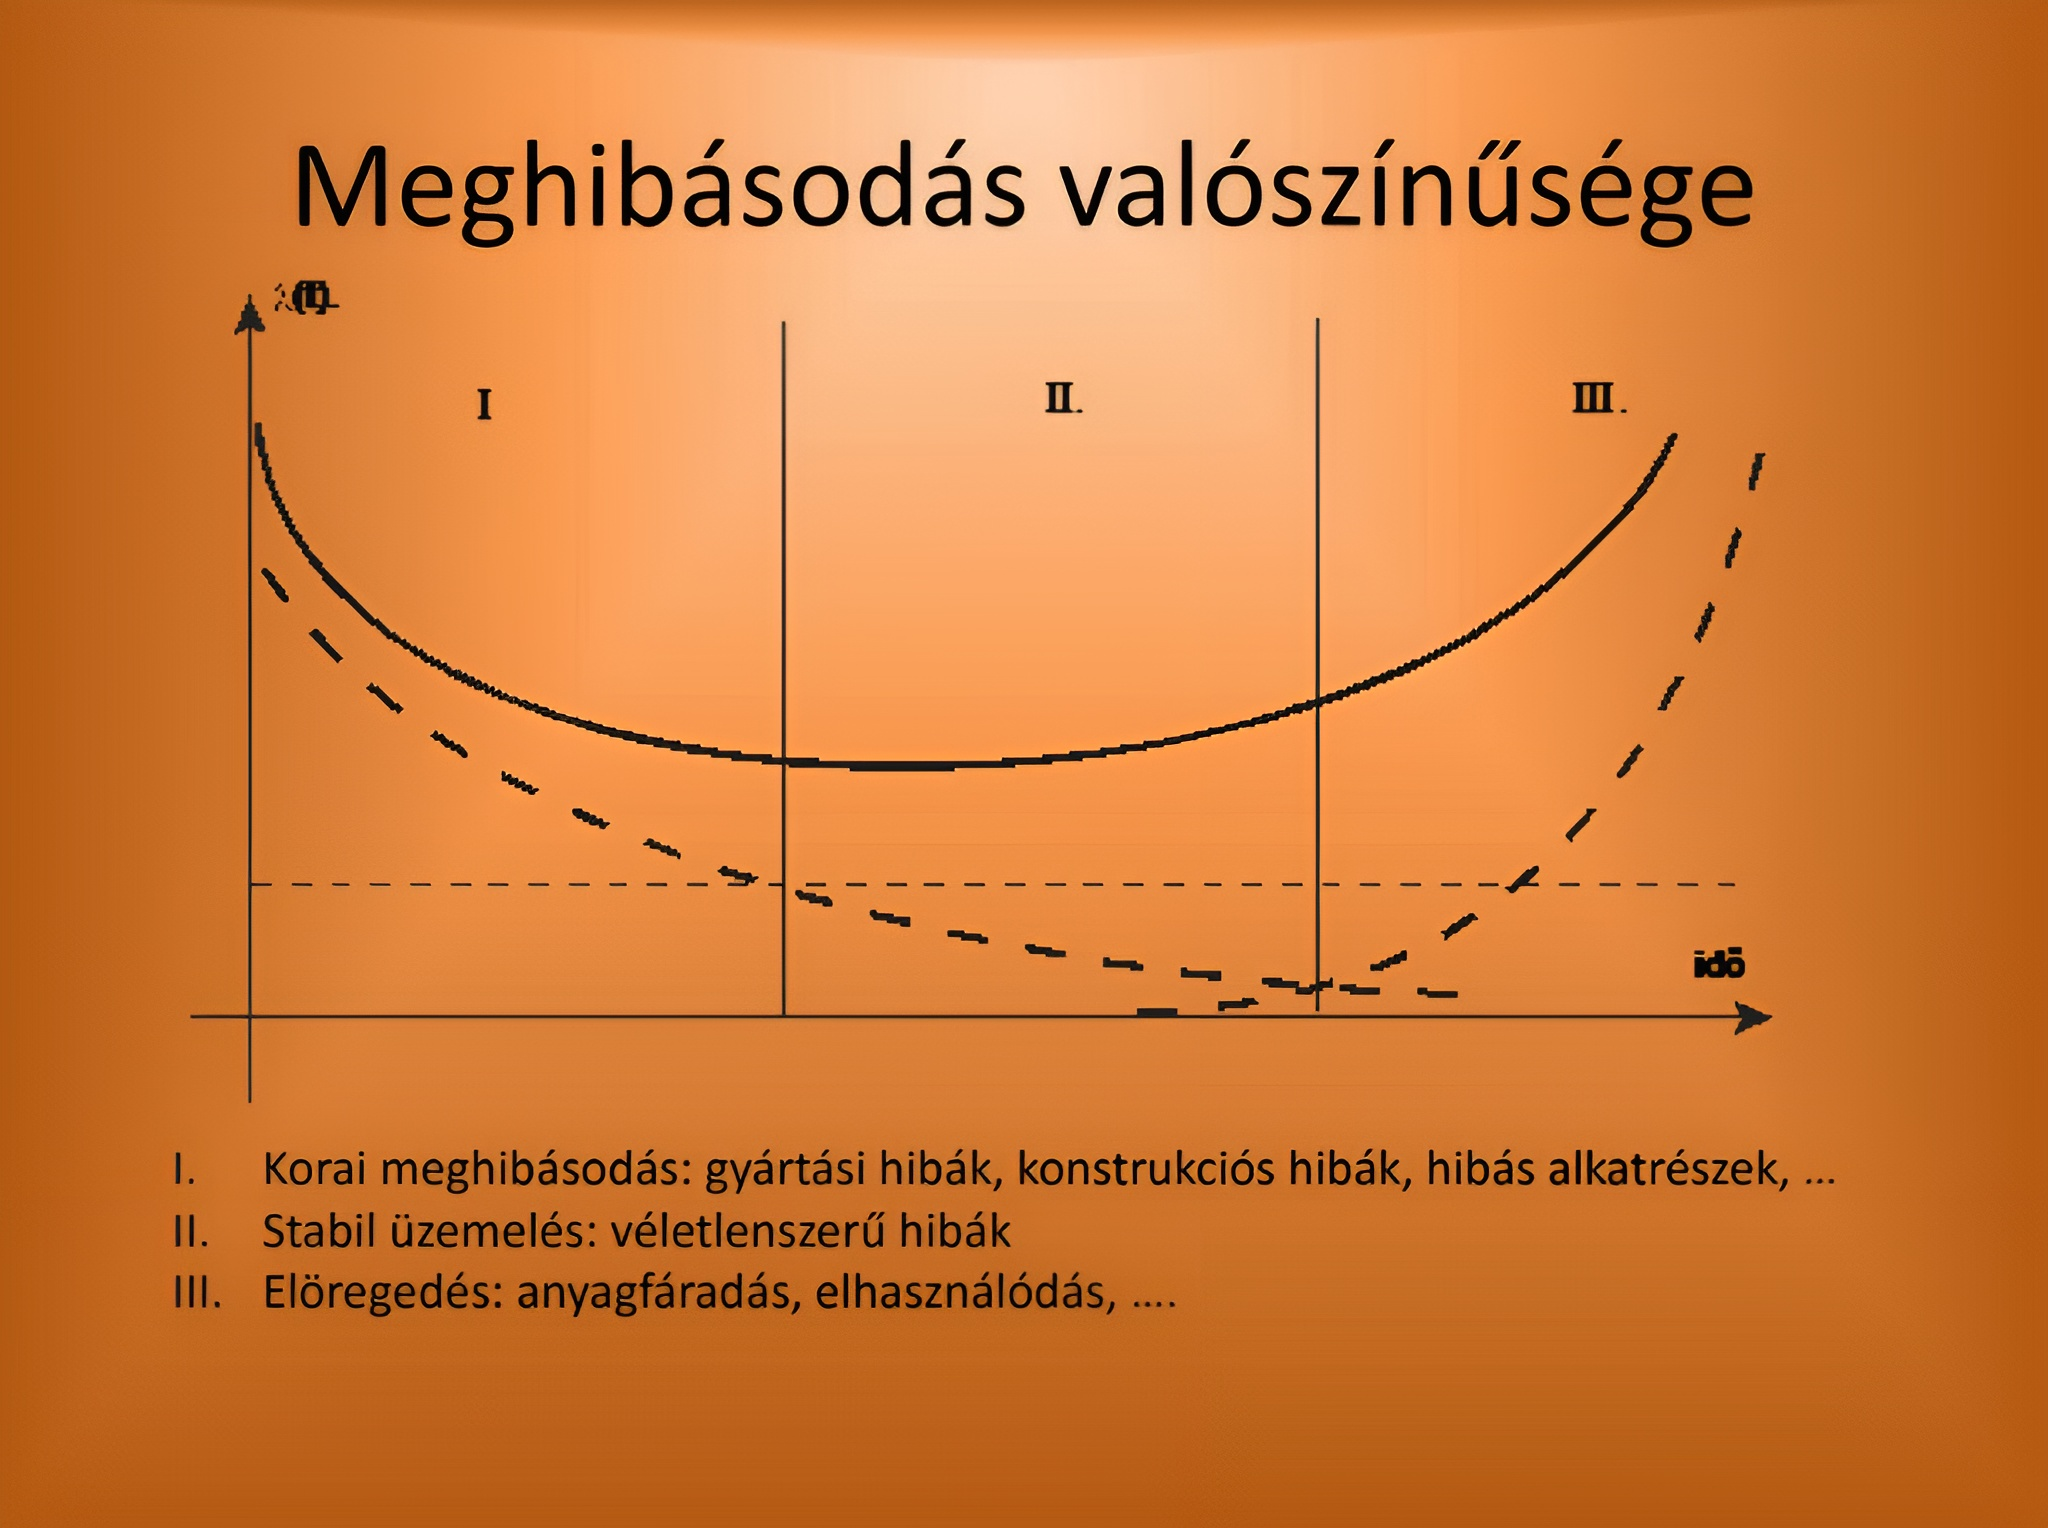
\includegraphics[width=0.7\textwidth]{kep/kep22.png}
    \caption{Kád görbe}
    \label{fig:kep22}
\end{figure}

\section{Összetett rendszerek megbízhtaósága (soros/párhuzamos kapcsolás)}

\begin{figure}[H]
    \centering
    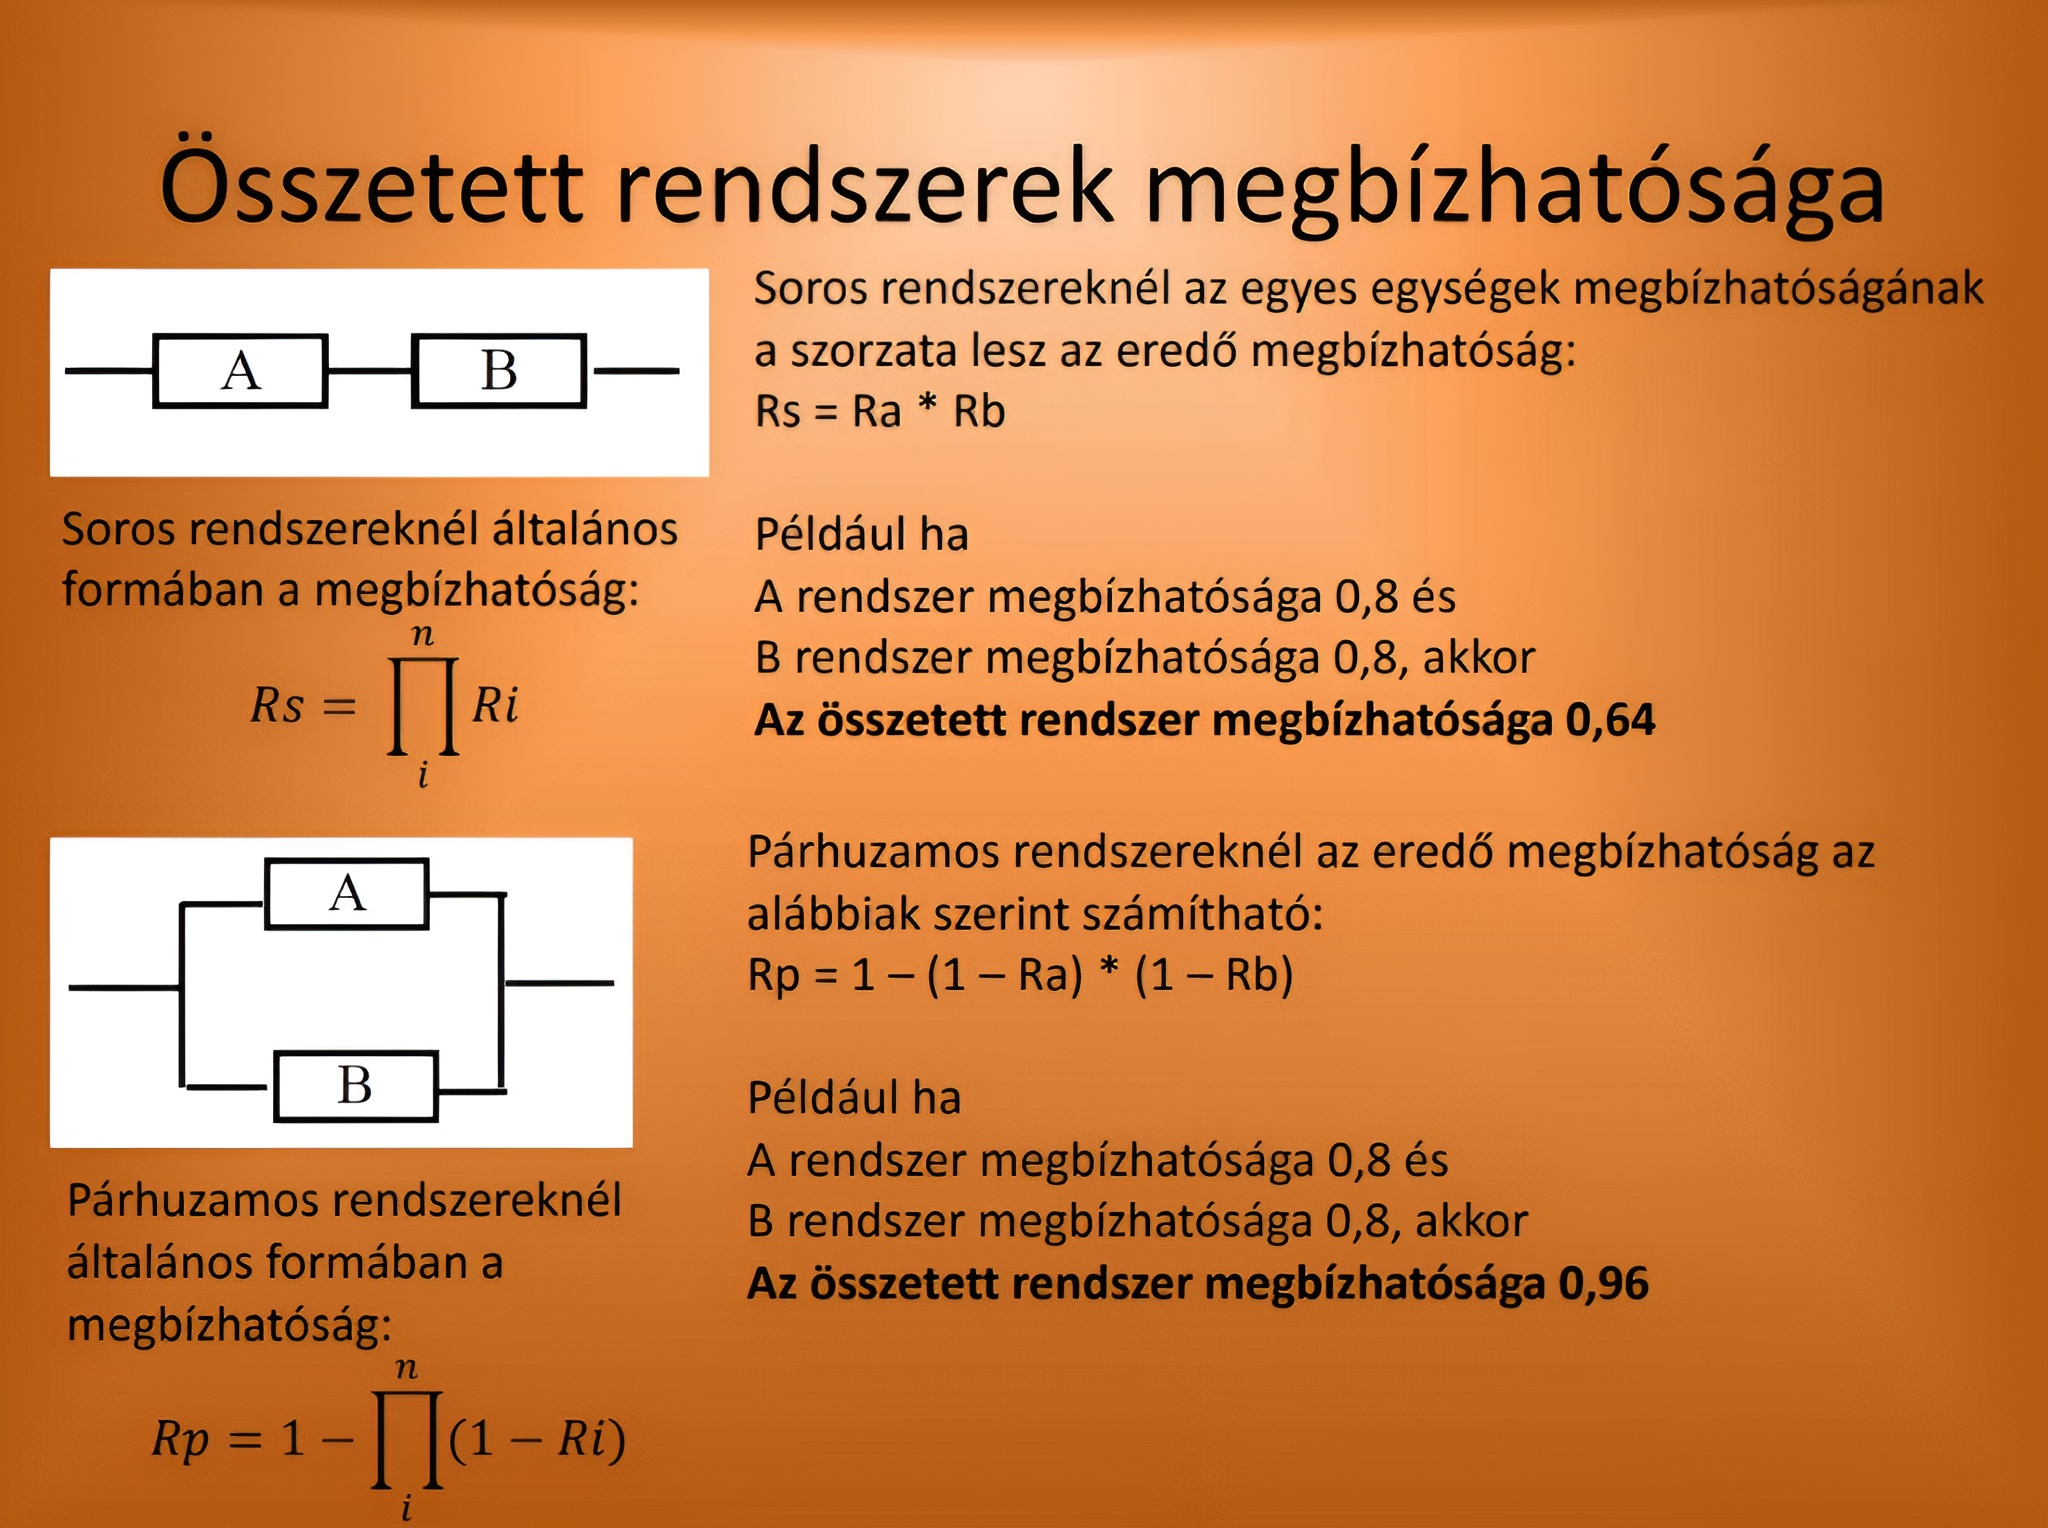
\includegraphics[width=0.7\textwidth]{kep/kep23.png}
    \caption{Összetett rendszerek megbízhatósága}
    \label{fig:kep23}
\end{figure}

\subsection{Sorosan kapcsolt rendszerek megbízhatósága}

\begin{itemize}
    \item \textbf{Eredő megbízhatóság}
    \item \textbf{Sorba kapcsolva romlik a megbízhatóság}
    \item \textbf{Rs = Ra * Rb}
    \item Pl: két eszköz megbízhatósága önállóan 0,8 és 0,8 sorba kapcsolva eredően 0,64
\end{itemize}

\subsection{Párhuzamosan kapcsolt rendszerek megbízhatósága}
\begin{itemize}
    \item \textbf{Rp = 1 – (1 – Ra) * (1 – Rb)}
    \item Pl: két eszköz megbízhatósága önállóan 0,8 akkor párhuzamosan kapcsolva összesen 0,96
\end{itemize}

\section{Redundáns energia ellátás}

\subsection{Soros kapcsolás}

\begin{figure}[H]
    \centering
    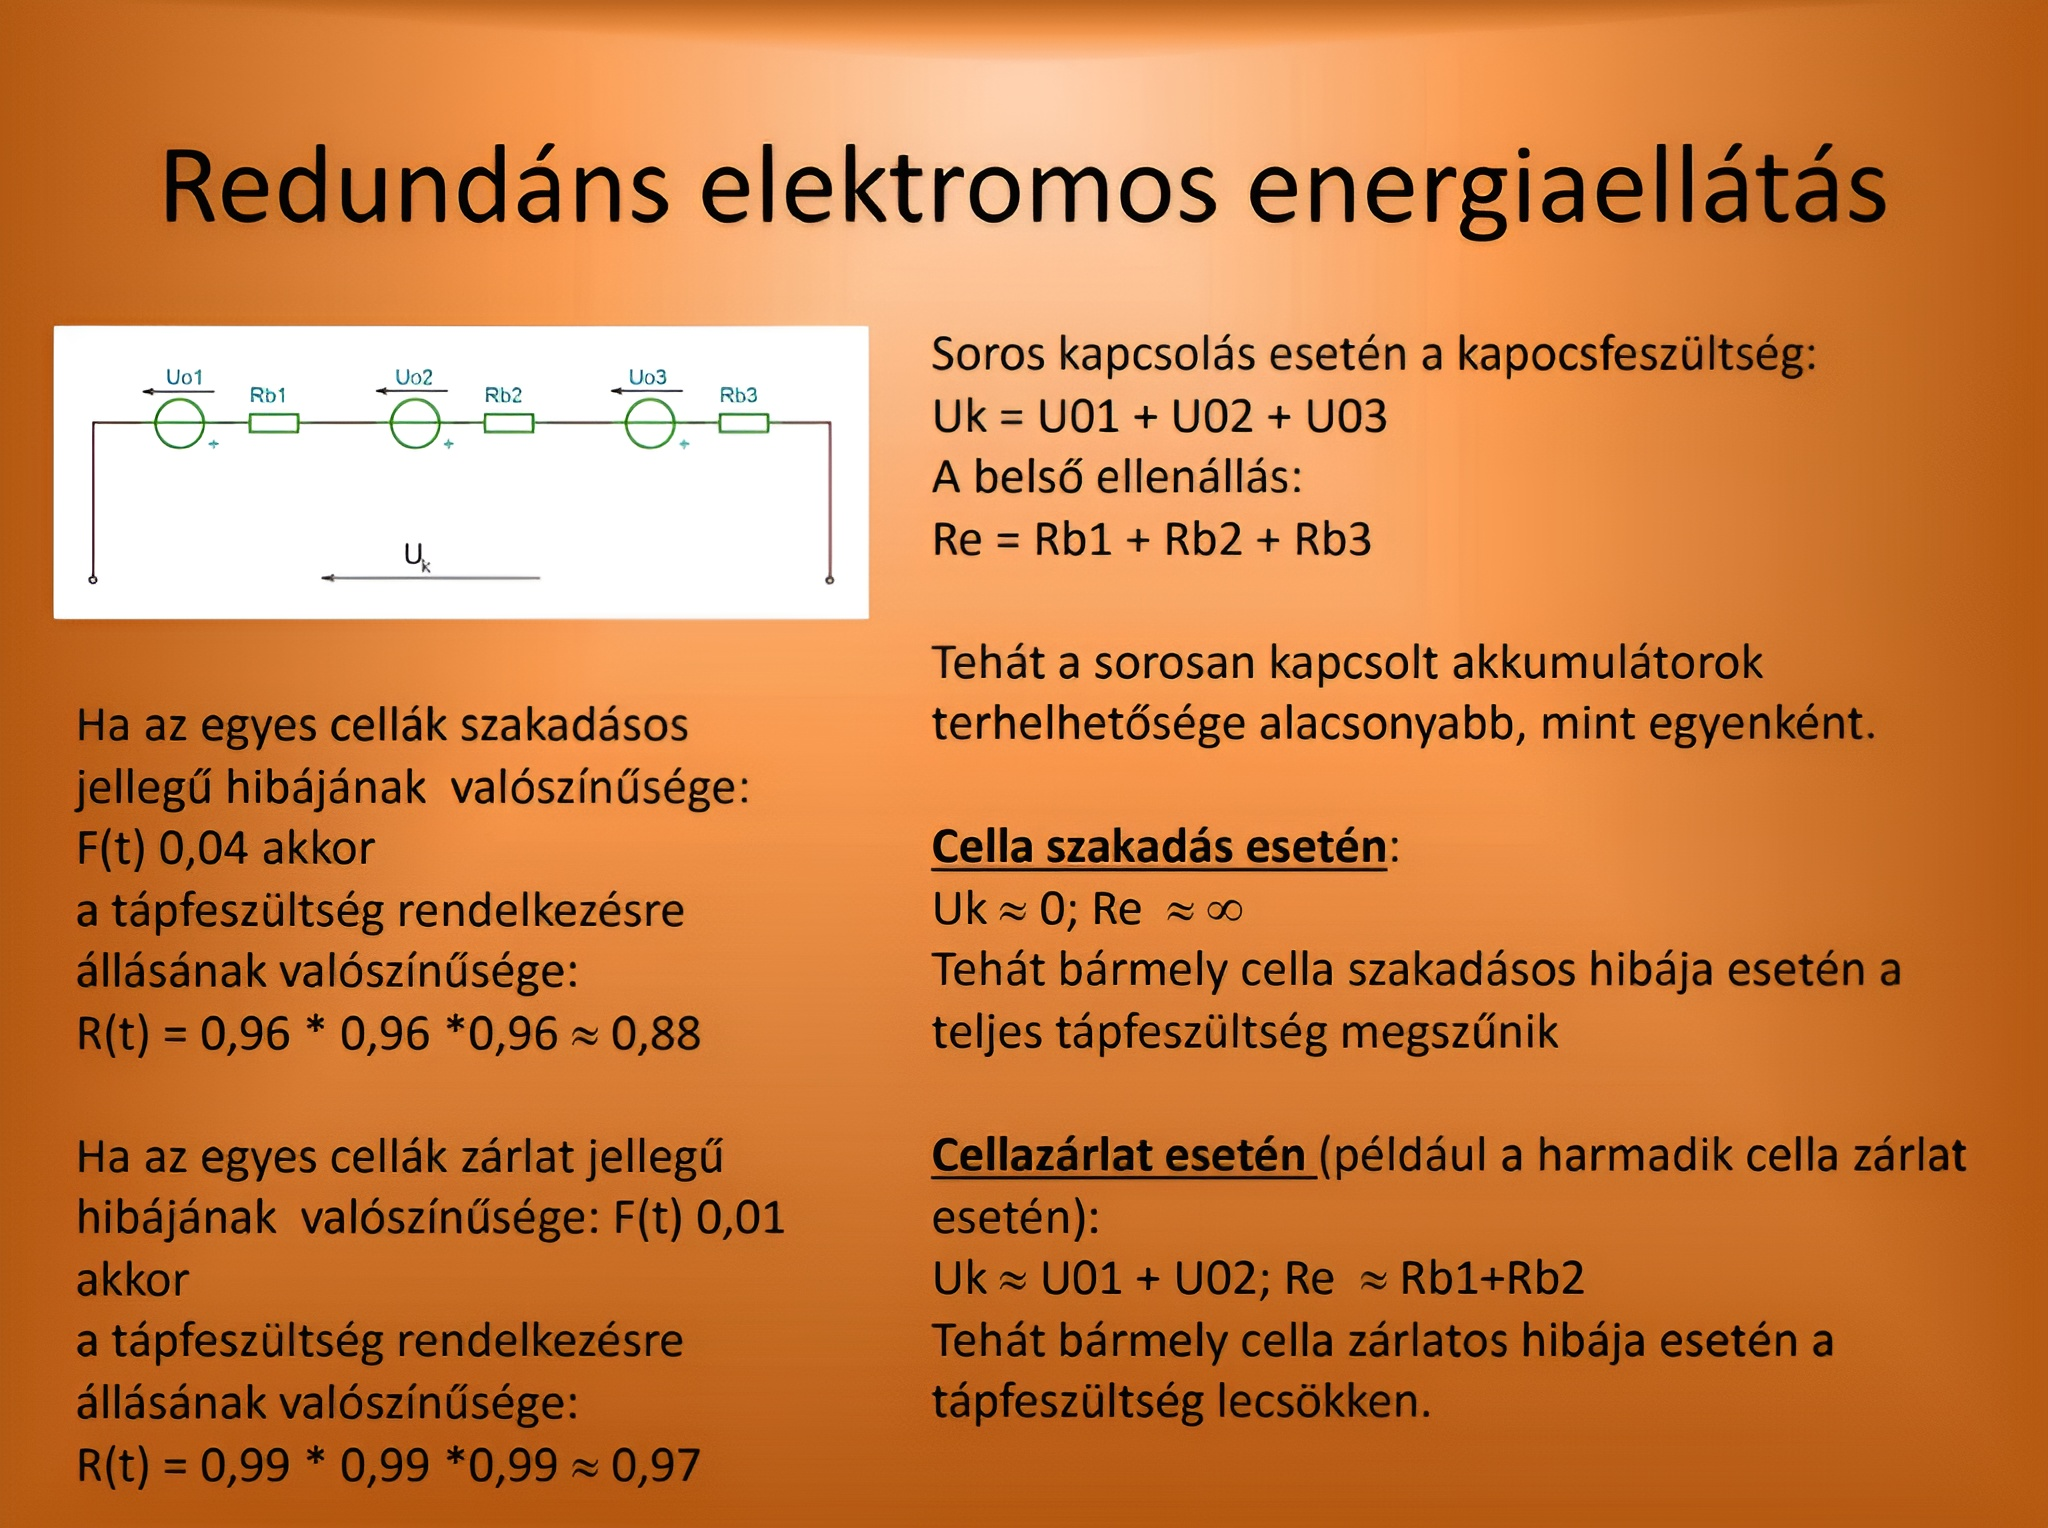
\includegraphics[width=0.7\textwidth]{kep/kep24.png}
    \caption{Redundáns energia ellátás - Soros kapcsolás}
    \label{fig:kep24}
\end{figure}

\begin{itemize}
    \item \textbf{Soros kapcsolás esetén a kapocsfeszültség: Uk = U1 + U2 + U3}
    \item \textbf{A belső ellenállás: Re = Rb1 + Rb2 + Rb3}
    \item \textbf{Cellaszakadás esetén: Uk = 0 ; Re = végtelen}
    \item \textbf{Zárlat esetén: Uk = U1 + U2 ; Re = Rb1 + Rb2}
\end{itemize}

\subsection{Párhuzamos kapcsolás}

\begin{figure}[H]
    \centering
    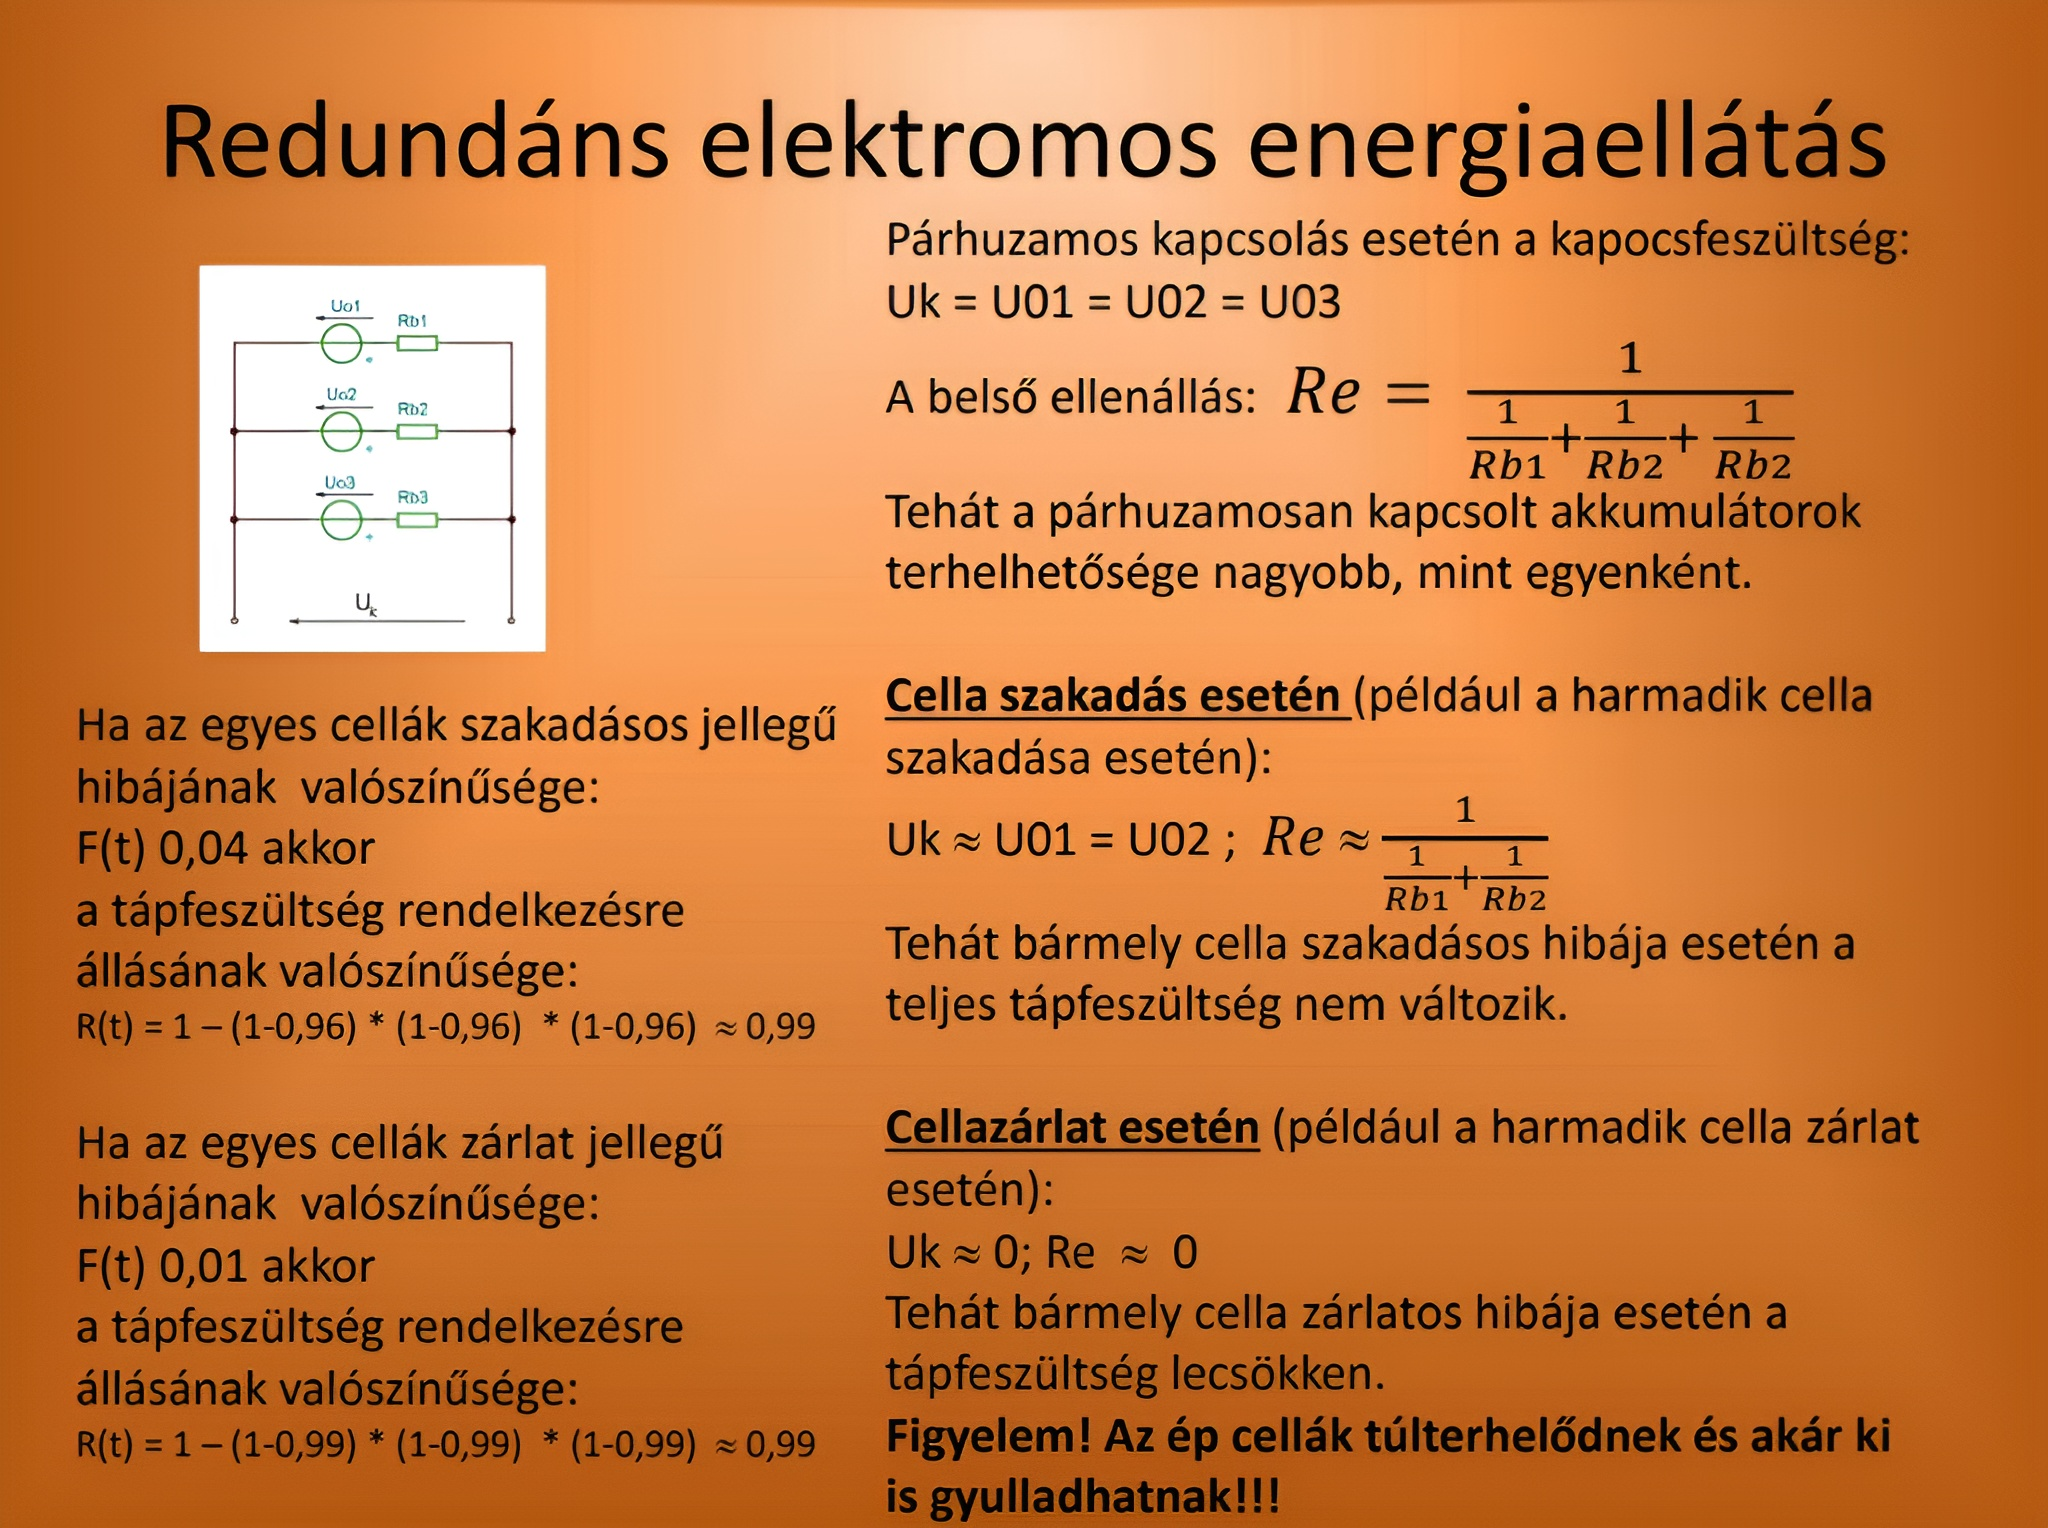
\includegraphics[width=0.7\textwidth]{kep/kep25.png}
    \caption{Redundáns energia ellátás - Párhuzamos kapcsolás}
    \label{fig:kep25}
\end{figure}

\begin{itemize}
    \item \textbf{Párhuzamos kapcsolás esetén a kapocsfeszültség: Uk = U1 = U2 = U3}
    \item \textbf{A belső ellenállás: Re = 1 / [ (1/Rb1) + (1/Rb2) + (1/Rb3) ]}
    \item Tehát a párhuzamosan kapcsolt akkumulátorok terhelhetősége nagyobb mint egyenként.
    \item \textbf{Cella szakadás esetén: Uk = U1 = U2 ; Re = 1 / [ (1/Rb1) + (1/Rb2) ]}
    \item \textbf{Cellazárlat esetén: Uk = 0 ; Re = 0}
    \item Tehát a tápfeszültség lecsökken, az ép cellák felizzanak, és ki is gyulladhatnak.
\end{itemize}

\subsection{Megbízhatóság cella szakadás esetén}

\begin{itemize}
    \item Ha a cella hiba valószínűsége Ft 0,04 akkor a tápfeszültség rendelkezésre állásának valószínűsége
    \item R(t) = 1 – (1-0,96) * (1-0,96) * (1-0,96) = 0,99
\end{itemize}

\subsection{Megbízhatóság cella zárlat esetén}

\begin{itemize}
    \item Ha a cella hiba valószínűsége Ft 0,01 akkor a tápfeszültség rendelkezésre állásának valószínűsége
    \item R(t) = 1 – (1-0,99) * (1-0,99) * (1-0,99) = 0,99
\end{itemize}

\subsection{Cellák sorba és párhuzamosan kapcsolása egyidejűleg}

\begin{itemize}
    \item Előáll a kívánt (magasabb) feszültség, mellette nagy áramot is kapunk.
    \item Cella zárlat esetén az adott blokknak csökken a feszültsége egy cellányival, így a többi blokk elkezdi azt tölteni, mivel annak alacsonyabb a feszültsége.
    \item A következmény, hogy a maradék cellák túltöltésre kerülnek az adott blokkban.
    \item A túltöltés miatt gáz fejlődik a cellákban, ami a kigyulladásukhoz vezet.
    \item A megbízhatóság és a rendelkezésre állás javul, viszont súlyos következmény lehet, ha kigyullad vagy felrobban a cella.
\end{itemize}

\begin{figure}[H]
    \centering
    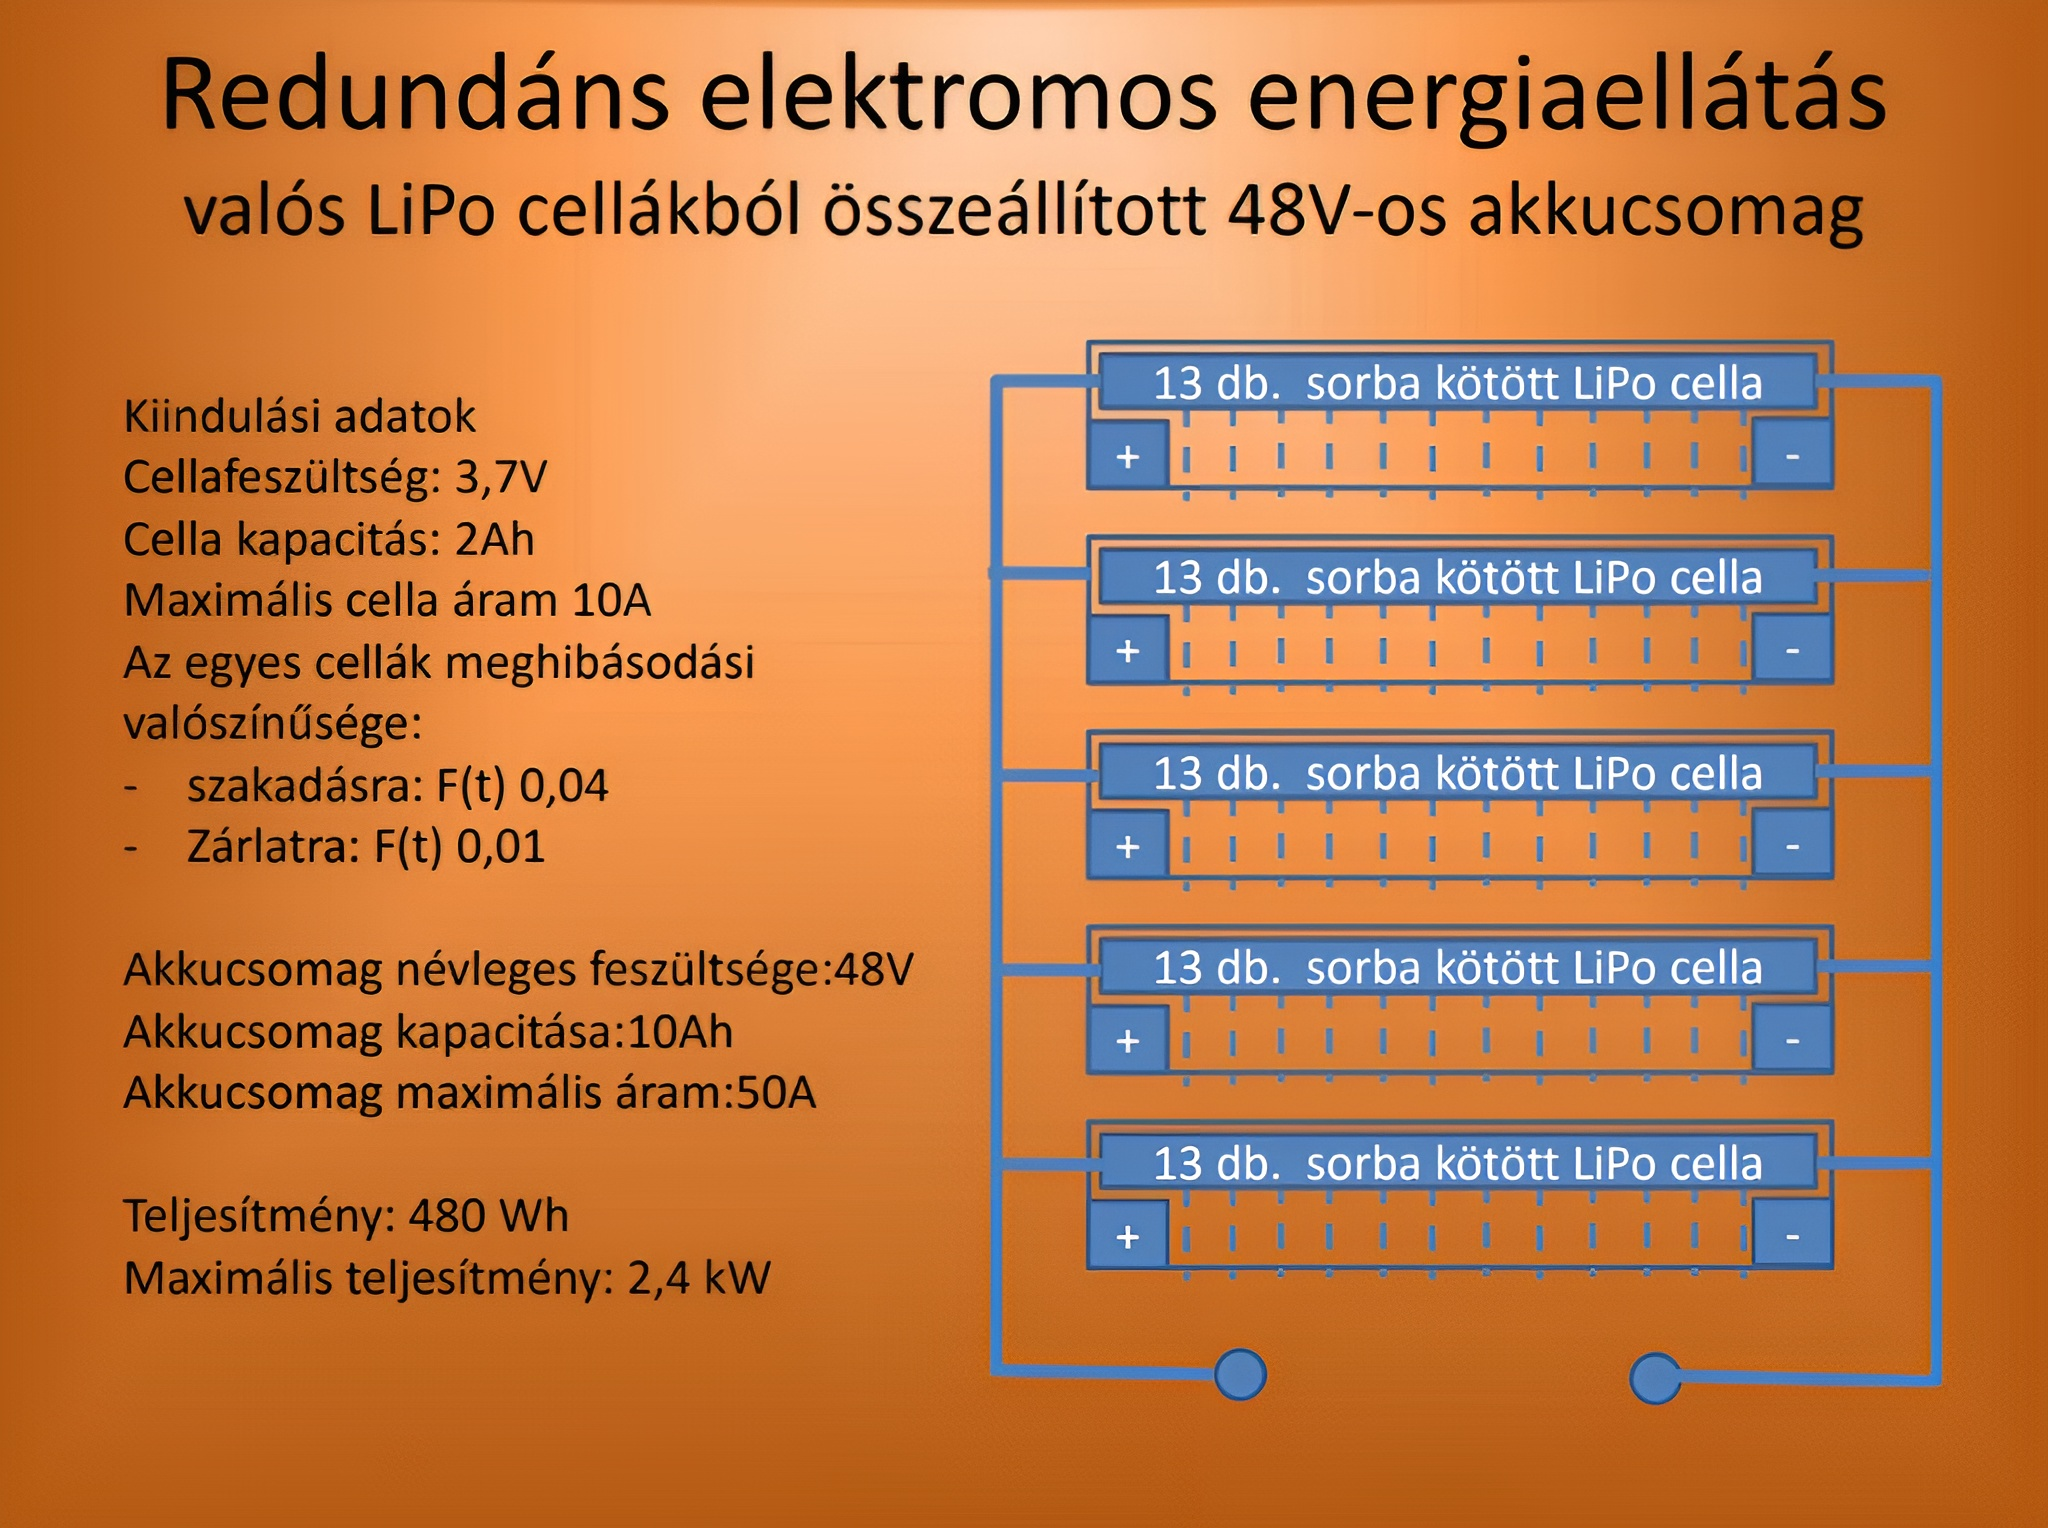
\includegraphics[width=0.7\textwidth]{kep/kep26.png}
    \caption{Redundáns energia ellátás I.}
    \label{fig:kep26}
\end{figure}

\begin{figure}[H]
    \centering
    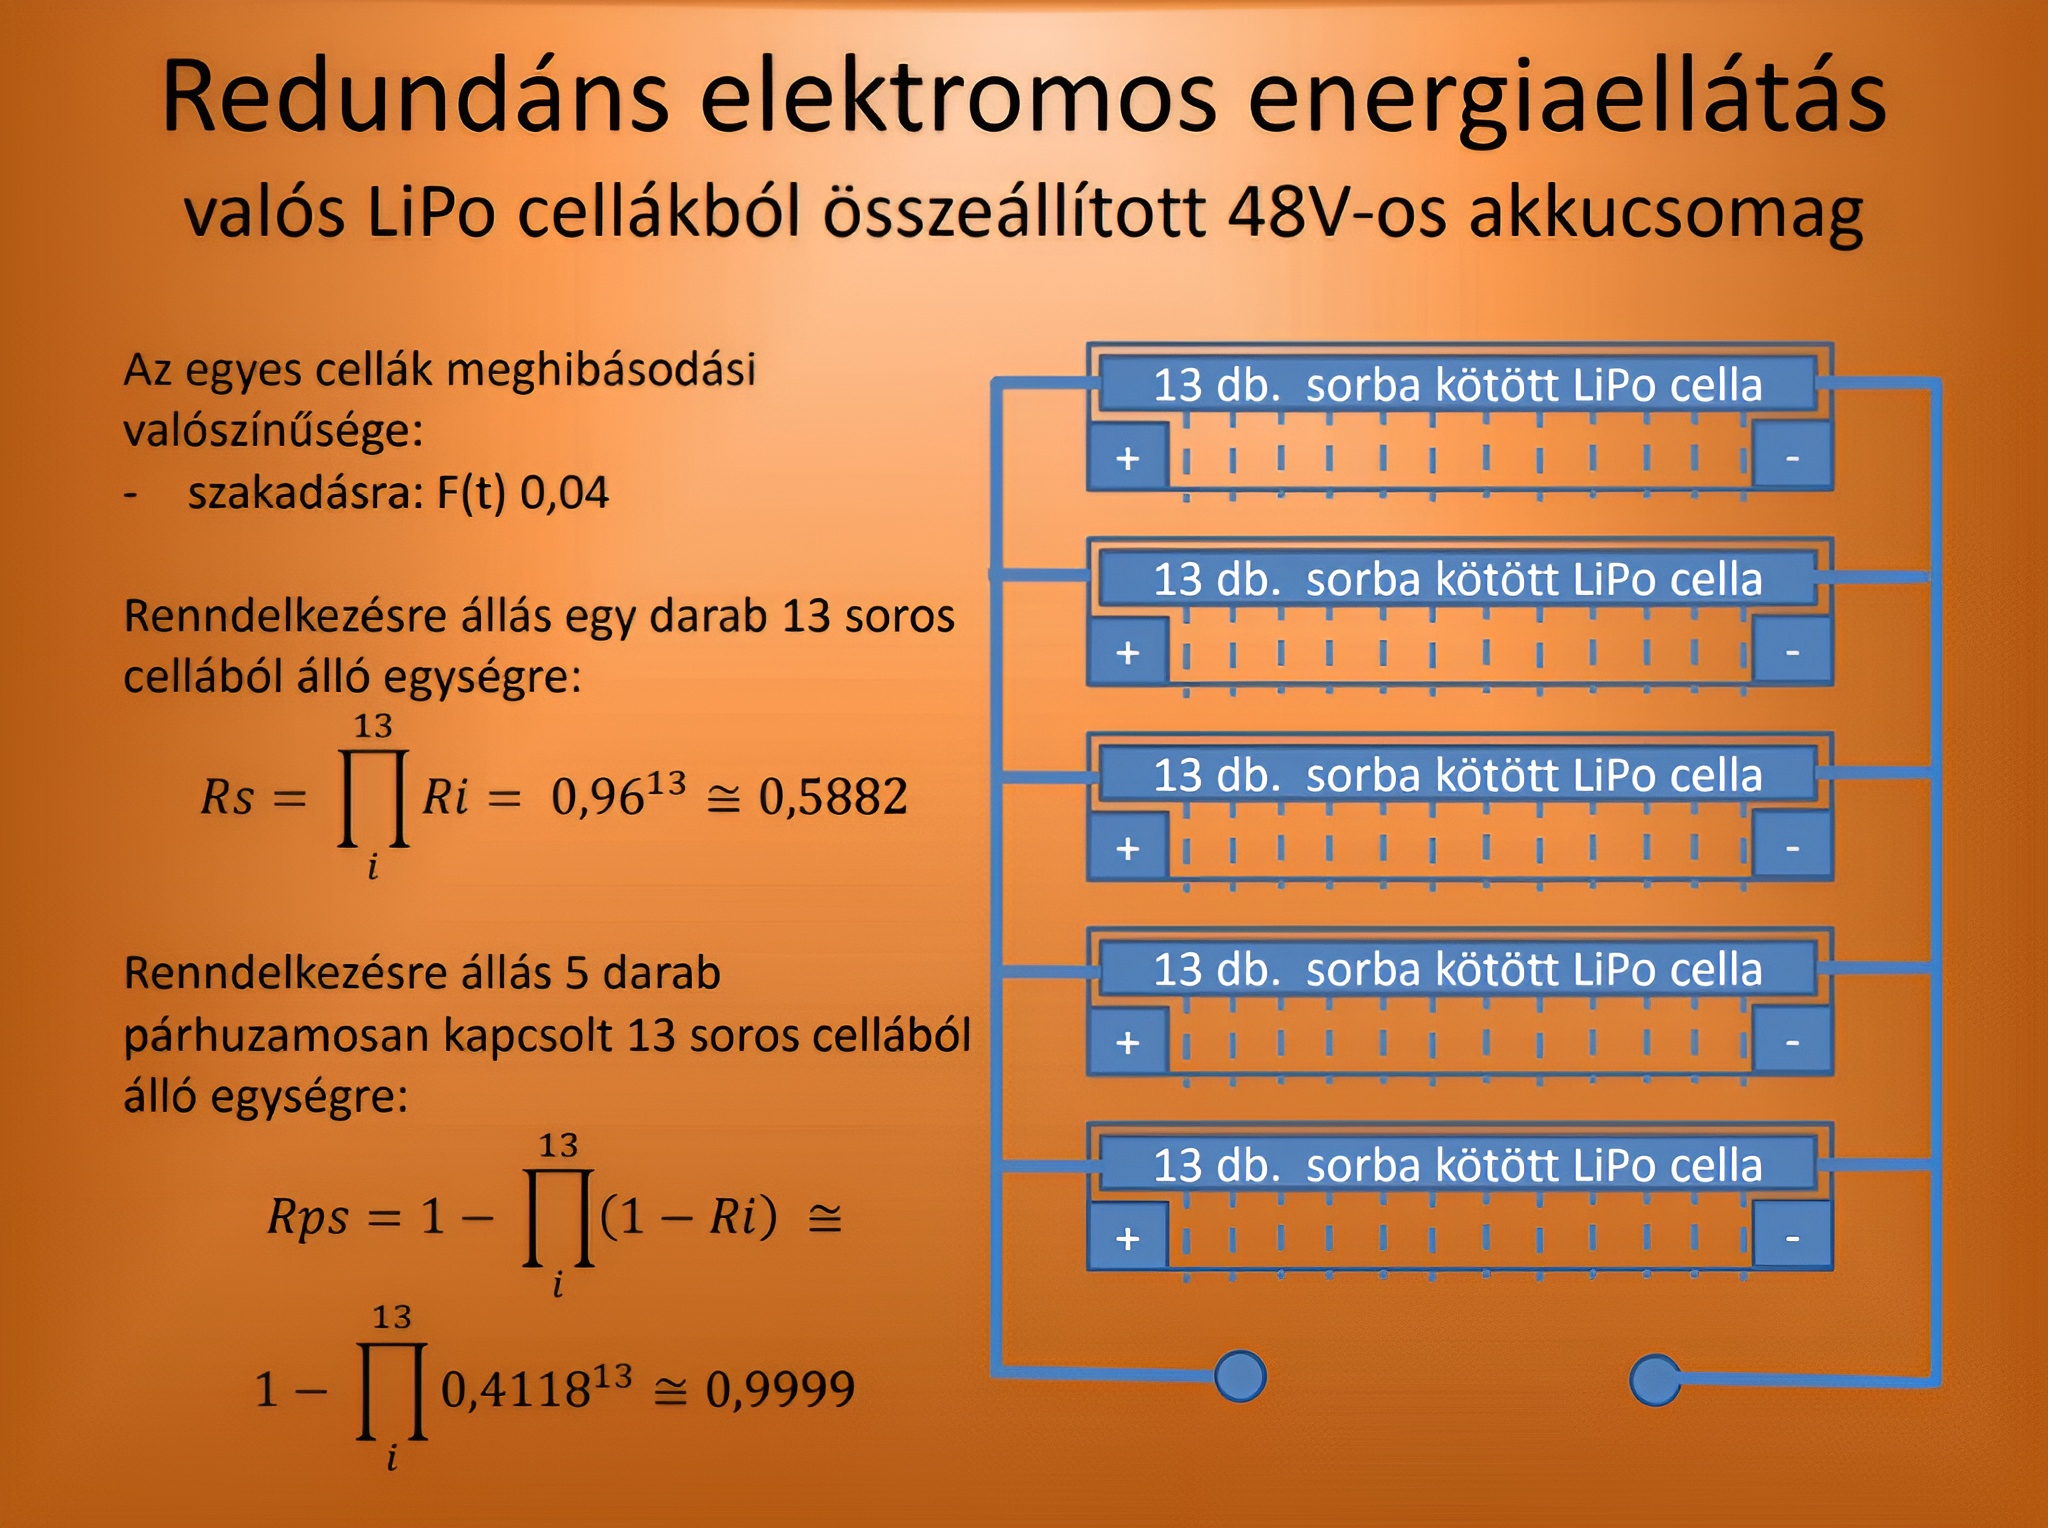
\includegraphics[width=0.7\textwidth]{kep/kep27.png}
    \caption{Redundáns energia ellátás II.}
    \label{fig:kep27}
\end{figure}

\begin{figure}[H]
    \centering
    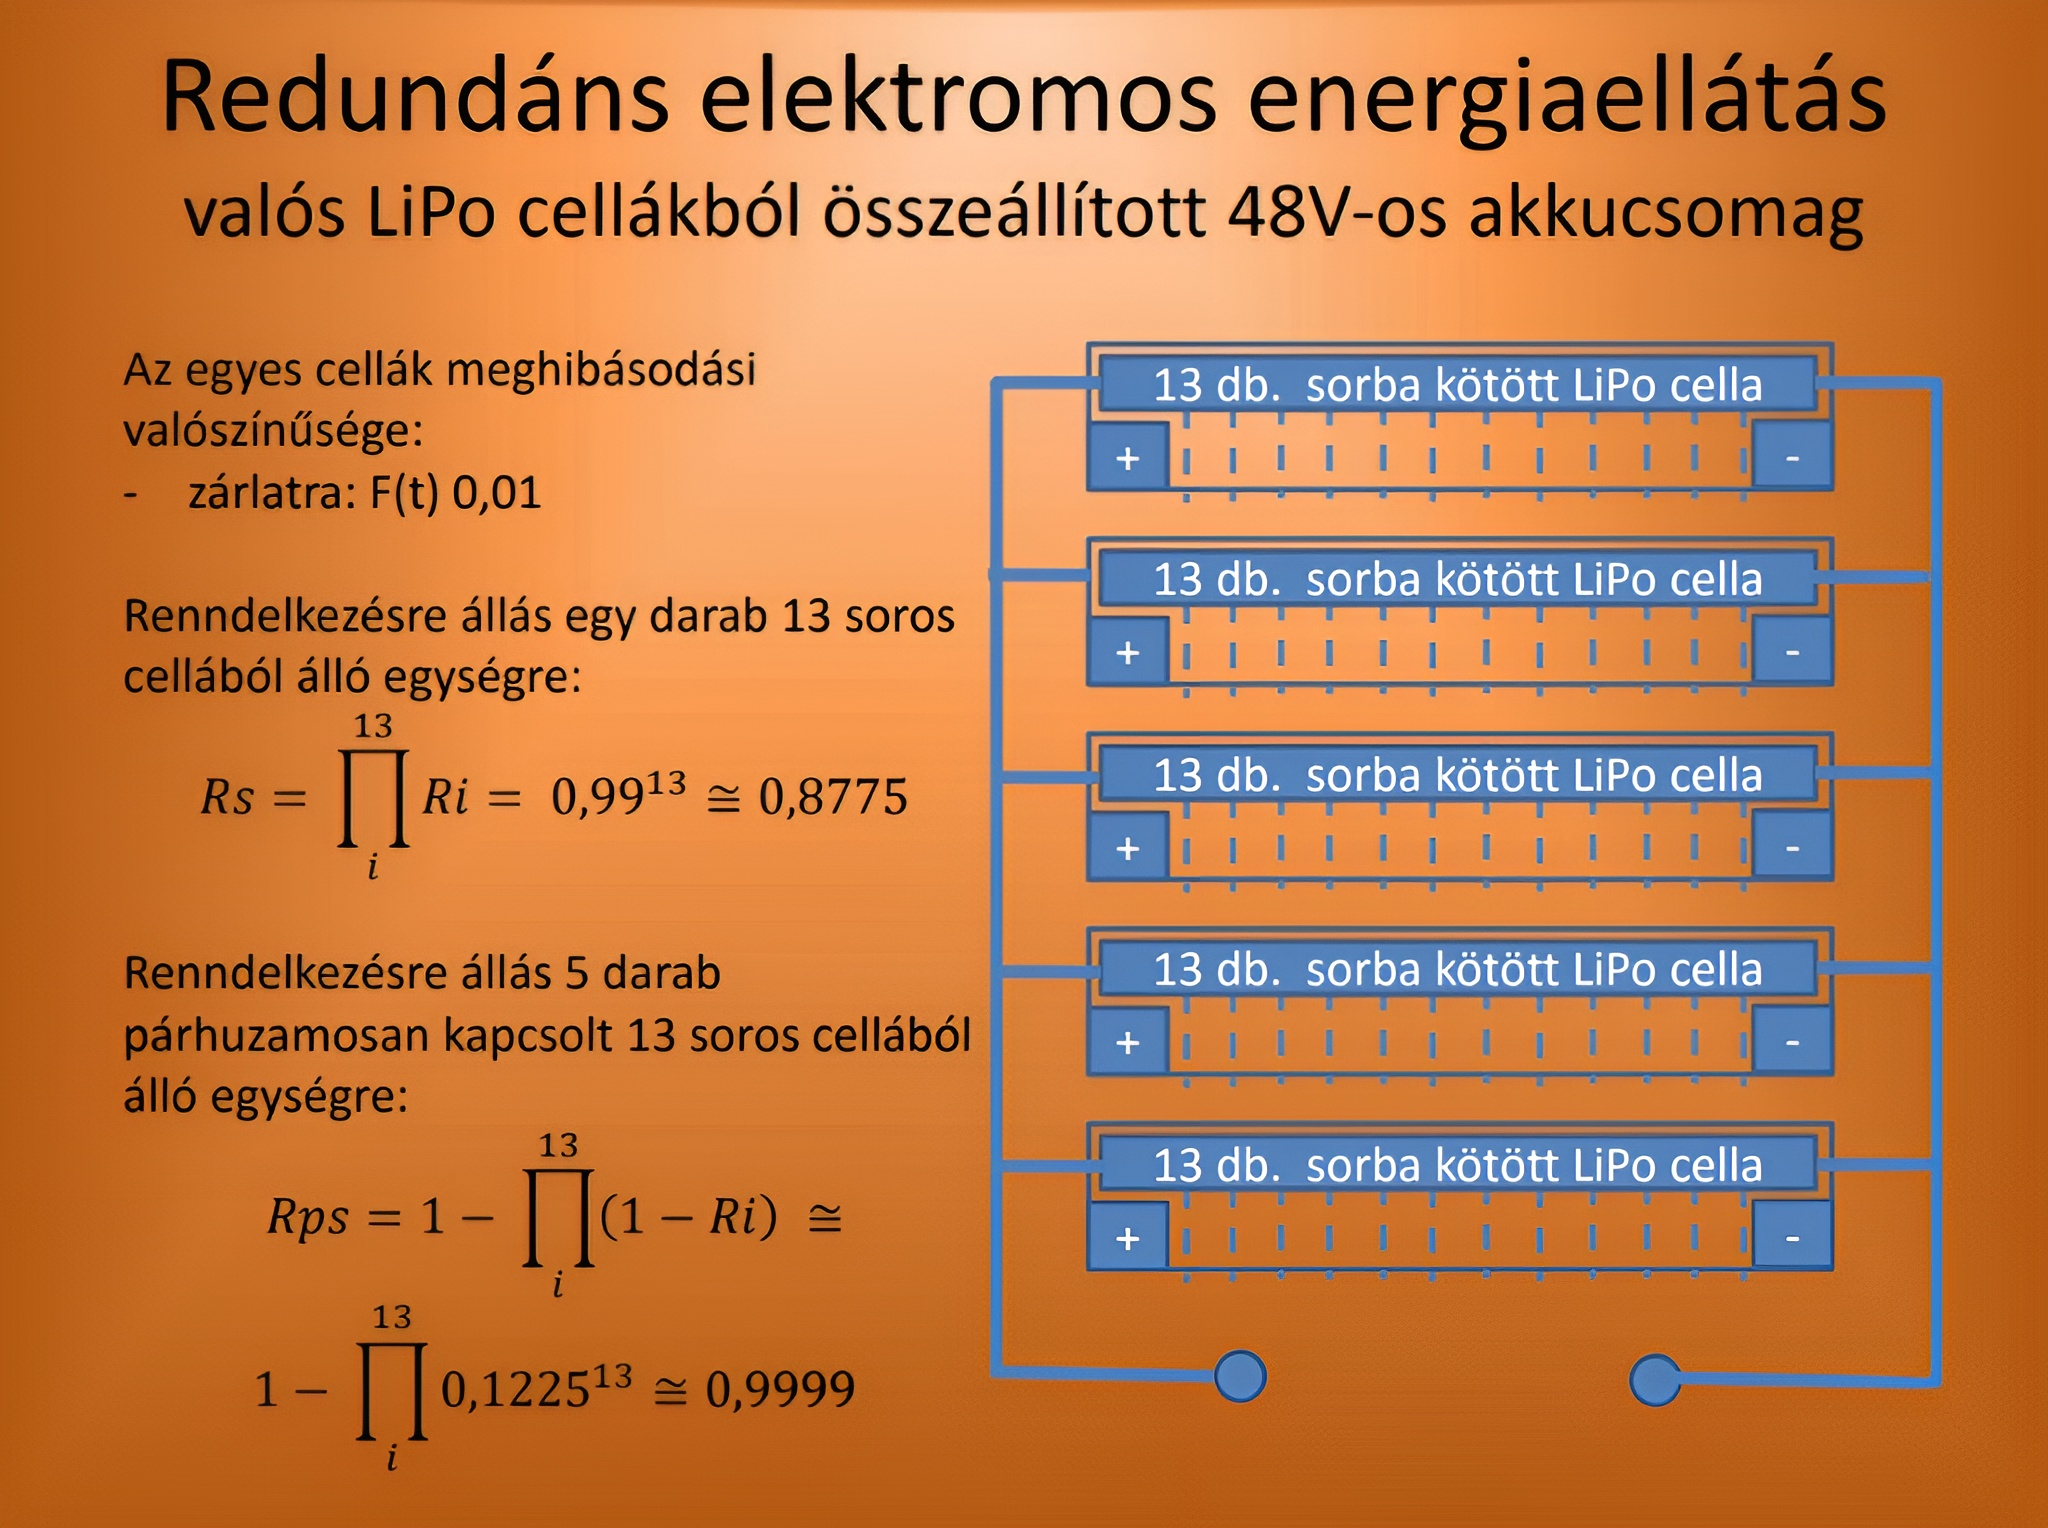
\includegraphics[width=0.7\textwidth]{kep/kep28.png}
    \caption{Redundáns energia ellátás III.}
    \label{fig:kep28}
\end{figure}

\begin{figure}[H]
    \centering
    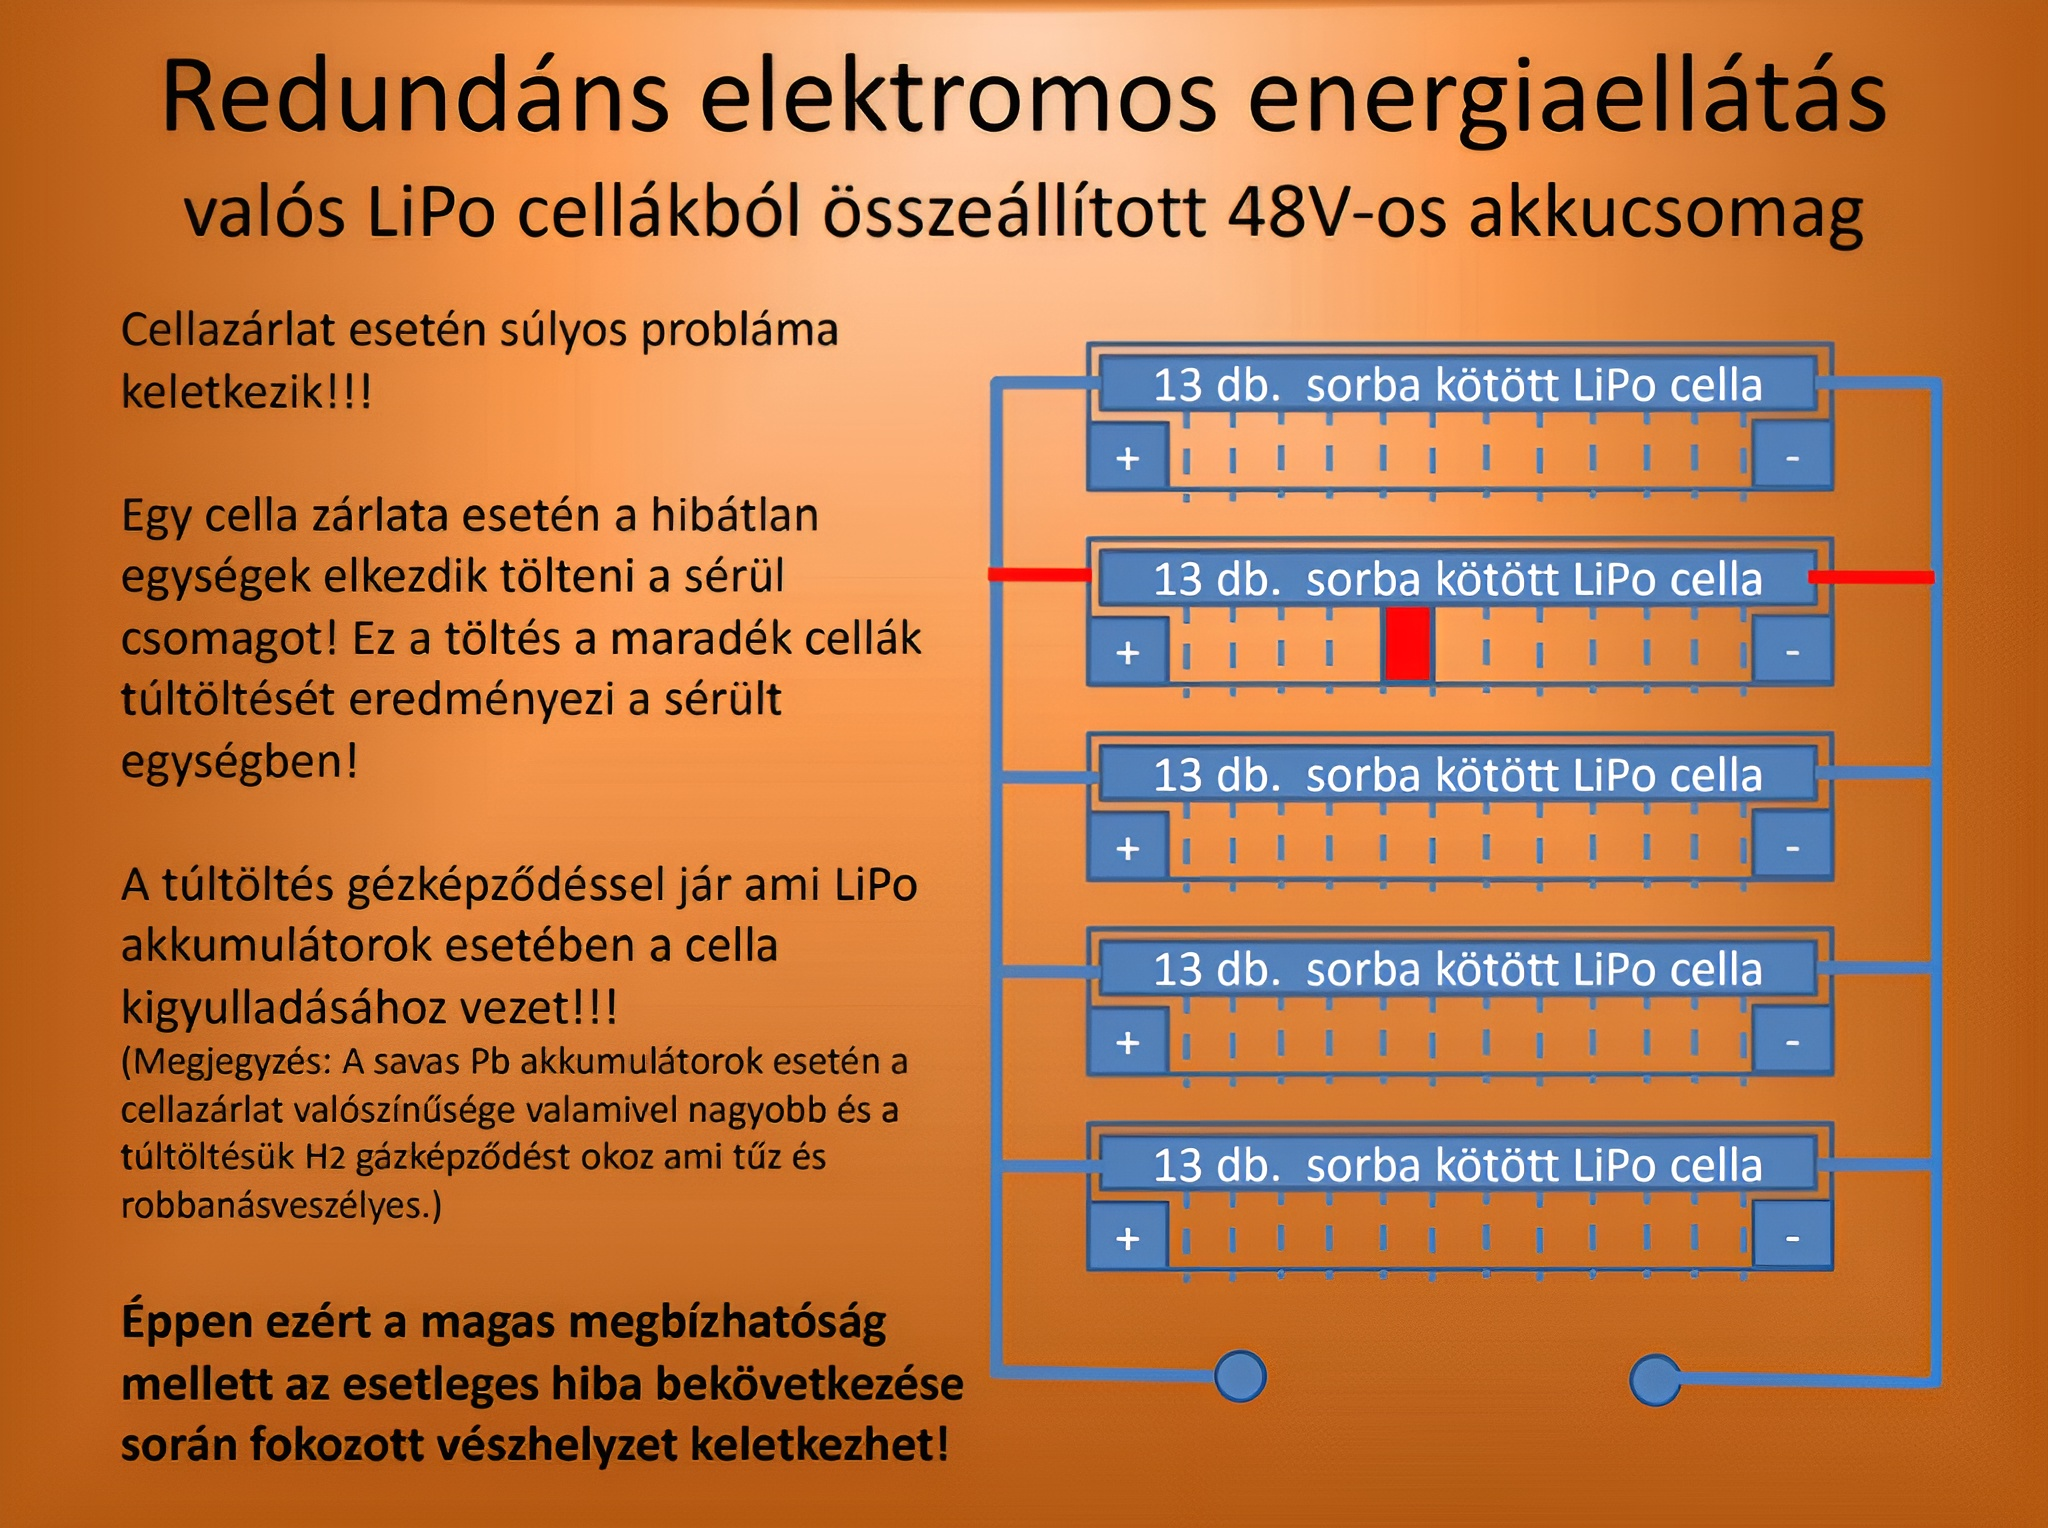
\includegraphics[width=0.7\textwidth]{kep/kep29.png}
    \caption{Redundáns energia ellátás IV.}
    \label{fig:kep29}
\end{figure}

\begin{figure}[H]
    \centering
    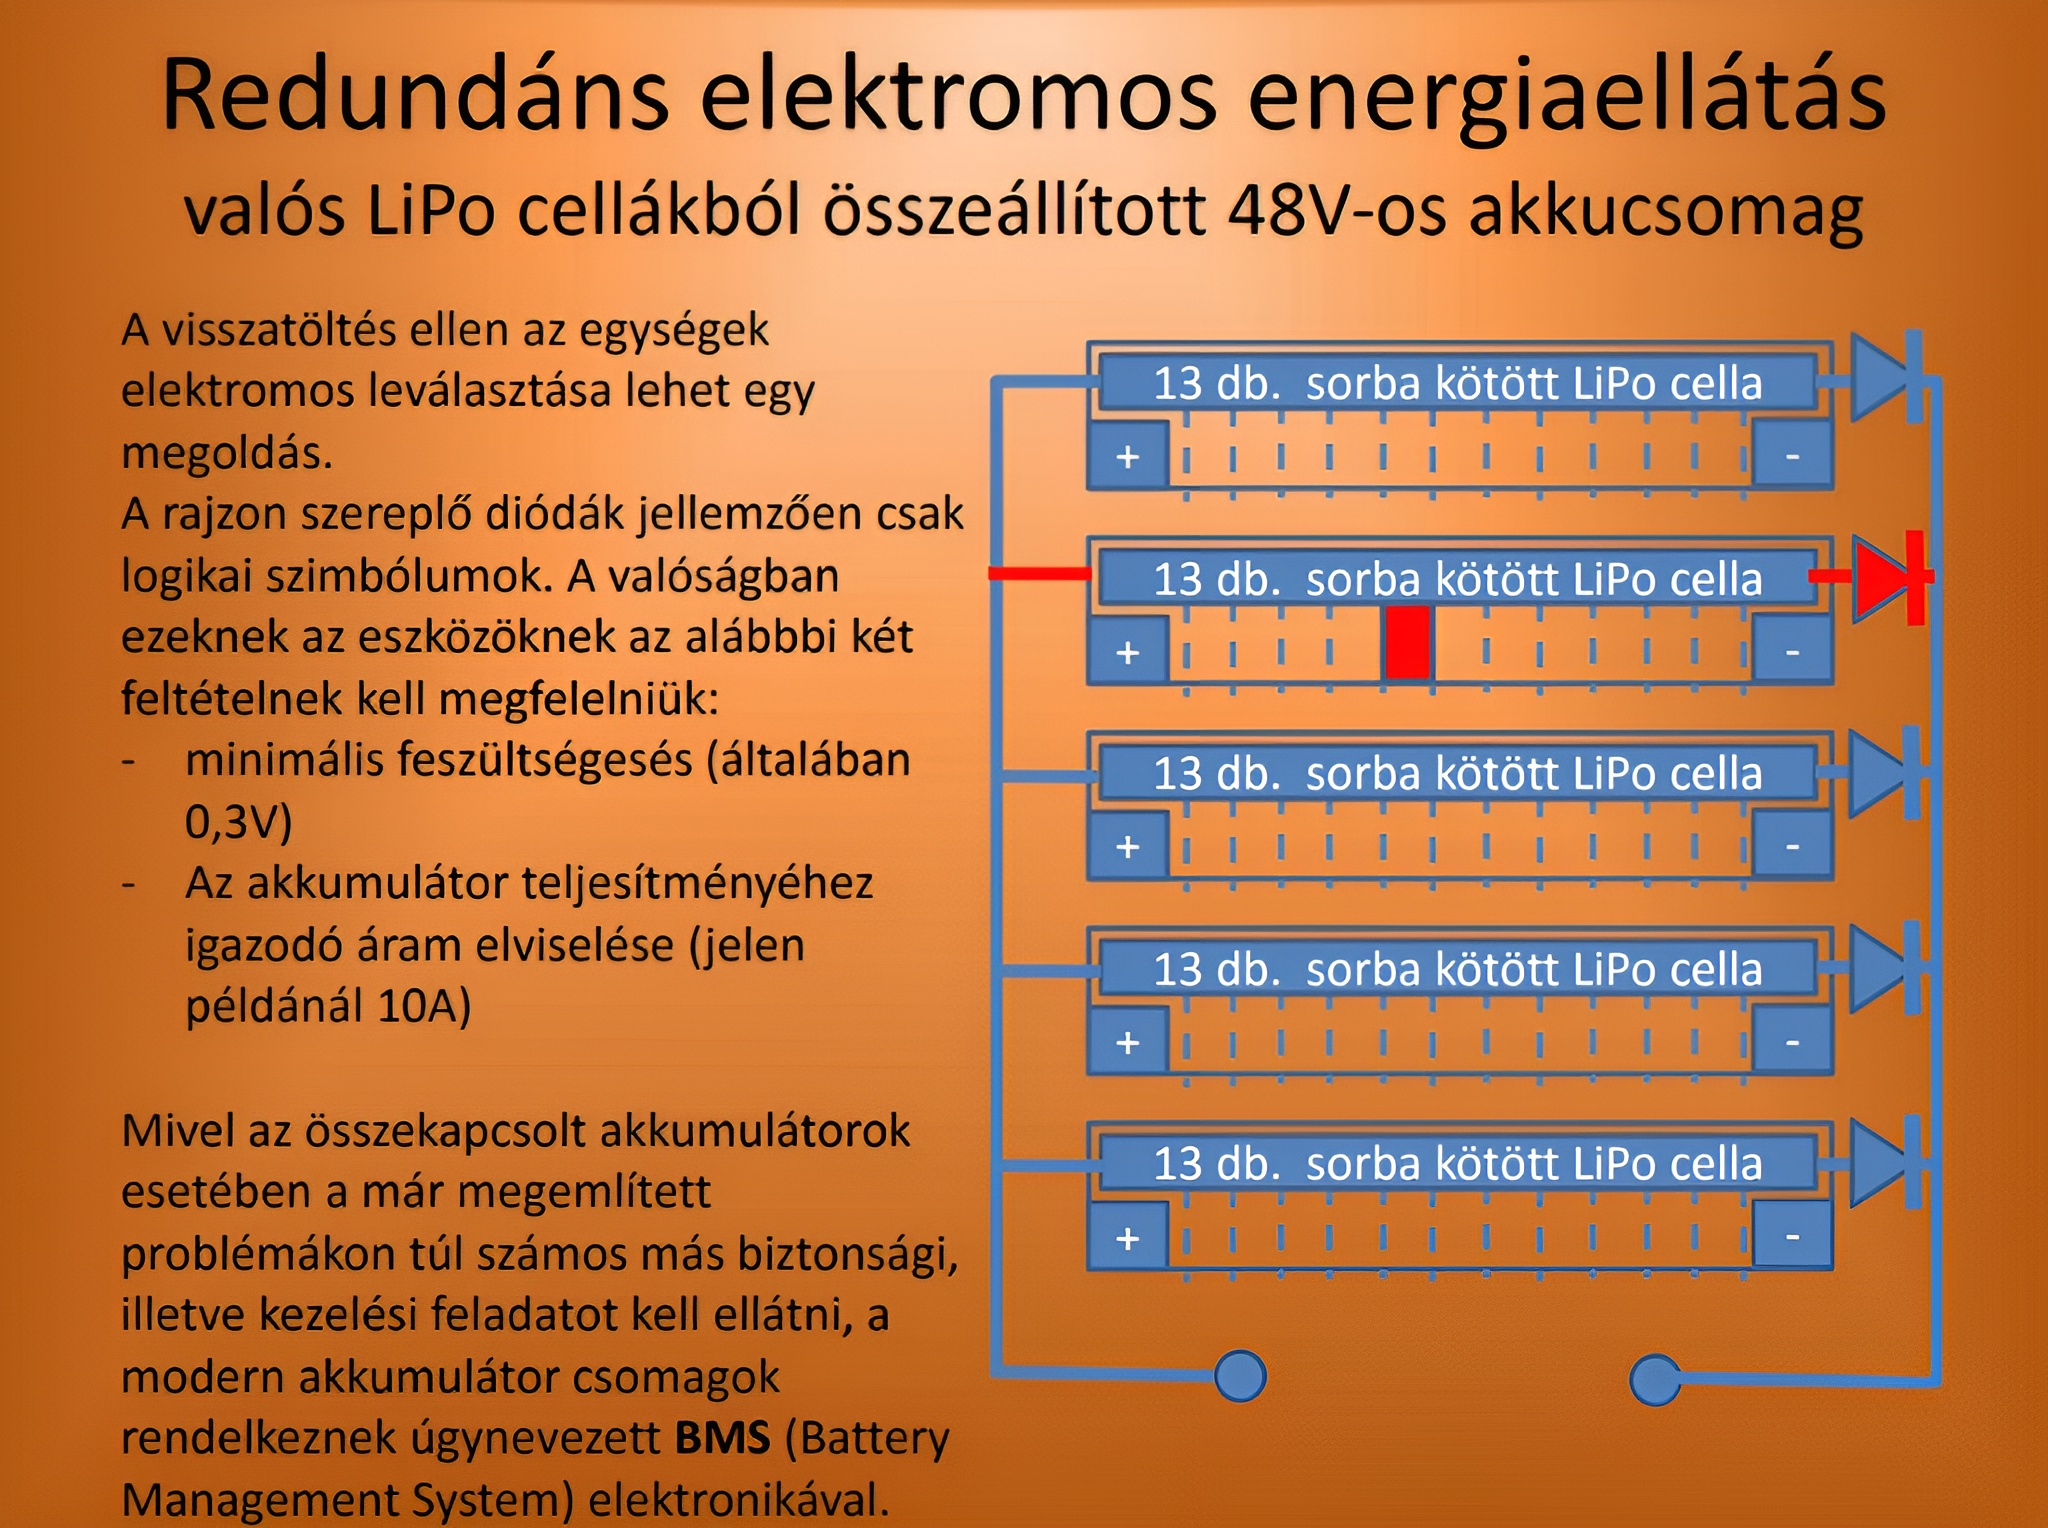
\includegraphics[width=0.7\textwidth]{kep/kep30.png}
    \caption{Redundáns energia ellátás V.}
    \label{fig:kep30}
\end{figure}

\subsection{Cellák élettartama és a biztonság növelése}

\begin{itemize}
    \item \textbf{BMS (Battery Management System)} használata.
    \item BMS használatával az egyes cellák élettartama nő, hiba esetén megvédi a többi cellát.
    \item Az akkukat nem engedi túlmerülni, vagy túltölteni.
    \item Amíg az akku élettartama nem romlott túlzott mértékben, a BMS el tudja fedni ezt.
    \item A BMS tartalékot hagy, amíg újak a cellák nagyobb tartalék lesz az akkukban, viszont ha romlani kezd a telep állapota, azonos teljesítményt tud nyújtani a BMS, amíg van tartalék. A felhasználó úgy érzi, mintha nem romlana az akku teljesítménye.
    \item Több féle BMS megvalósítás létezik, de a fő célja, hogy az egyes cellákat független egységként kezelje, viszont a felhasználó számára az összes cella egy akkuként legyen használható.
\end{itemize}

\begin{figure}[H]
    \centering
    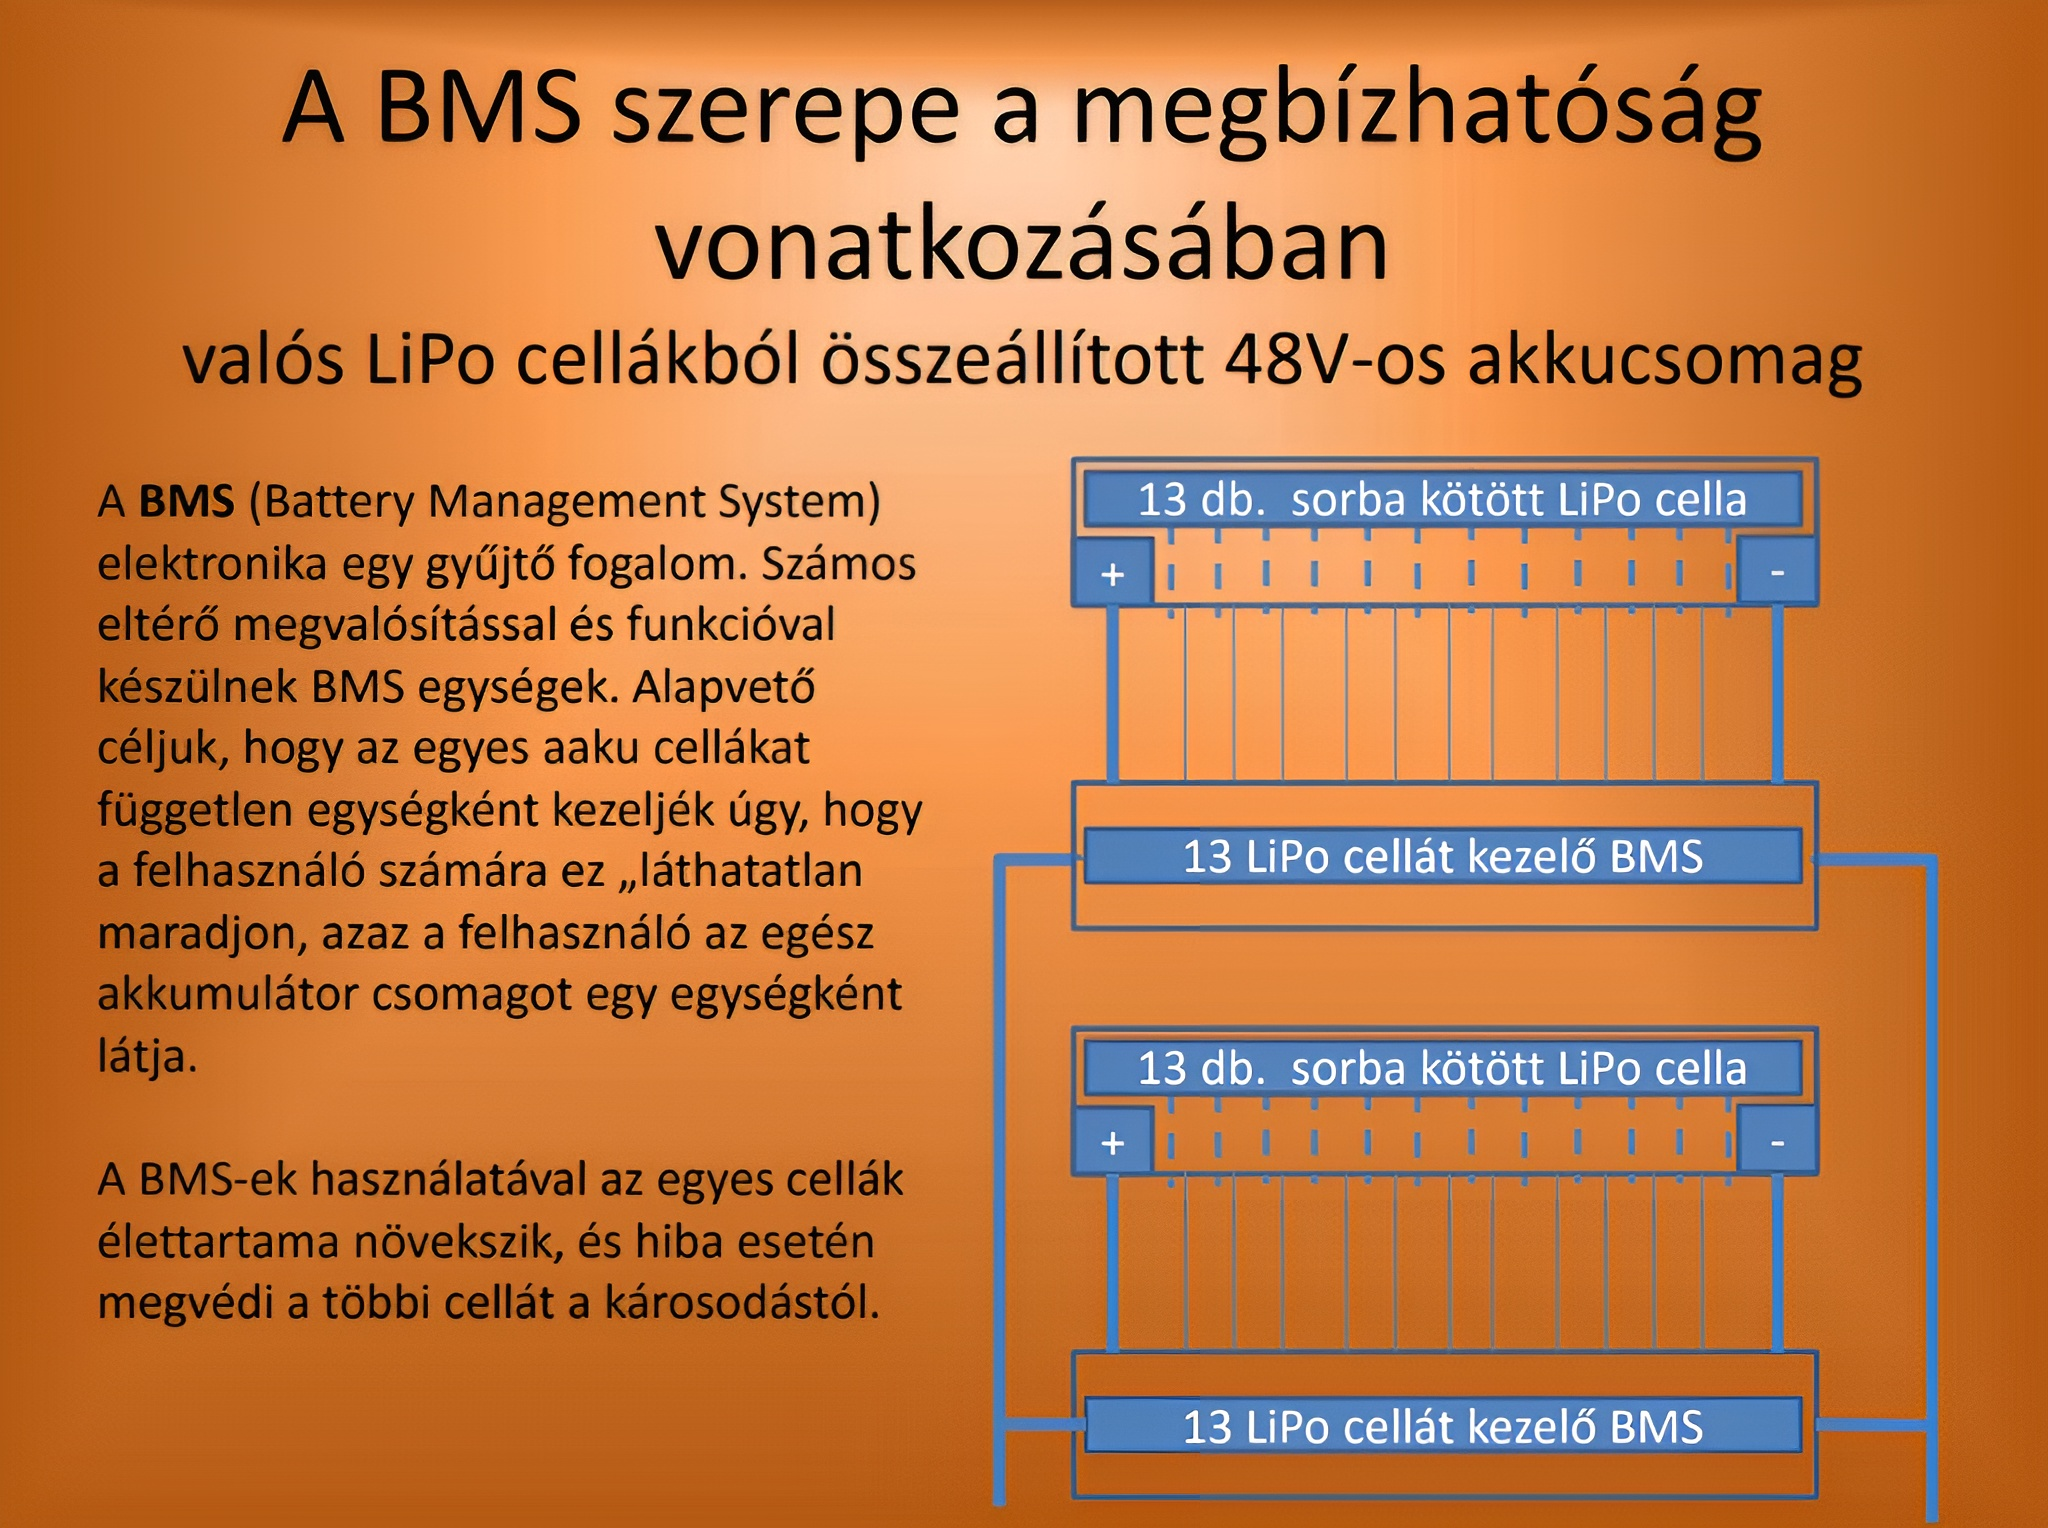
\includegraphics[width=0.7\textwidth]{kep/kep31.png}
    \caption{A BMS jellemzői I.}
    \label{fig:kep31}
\end{figure}

\begin{figure}[H]
    \centering
    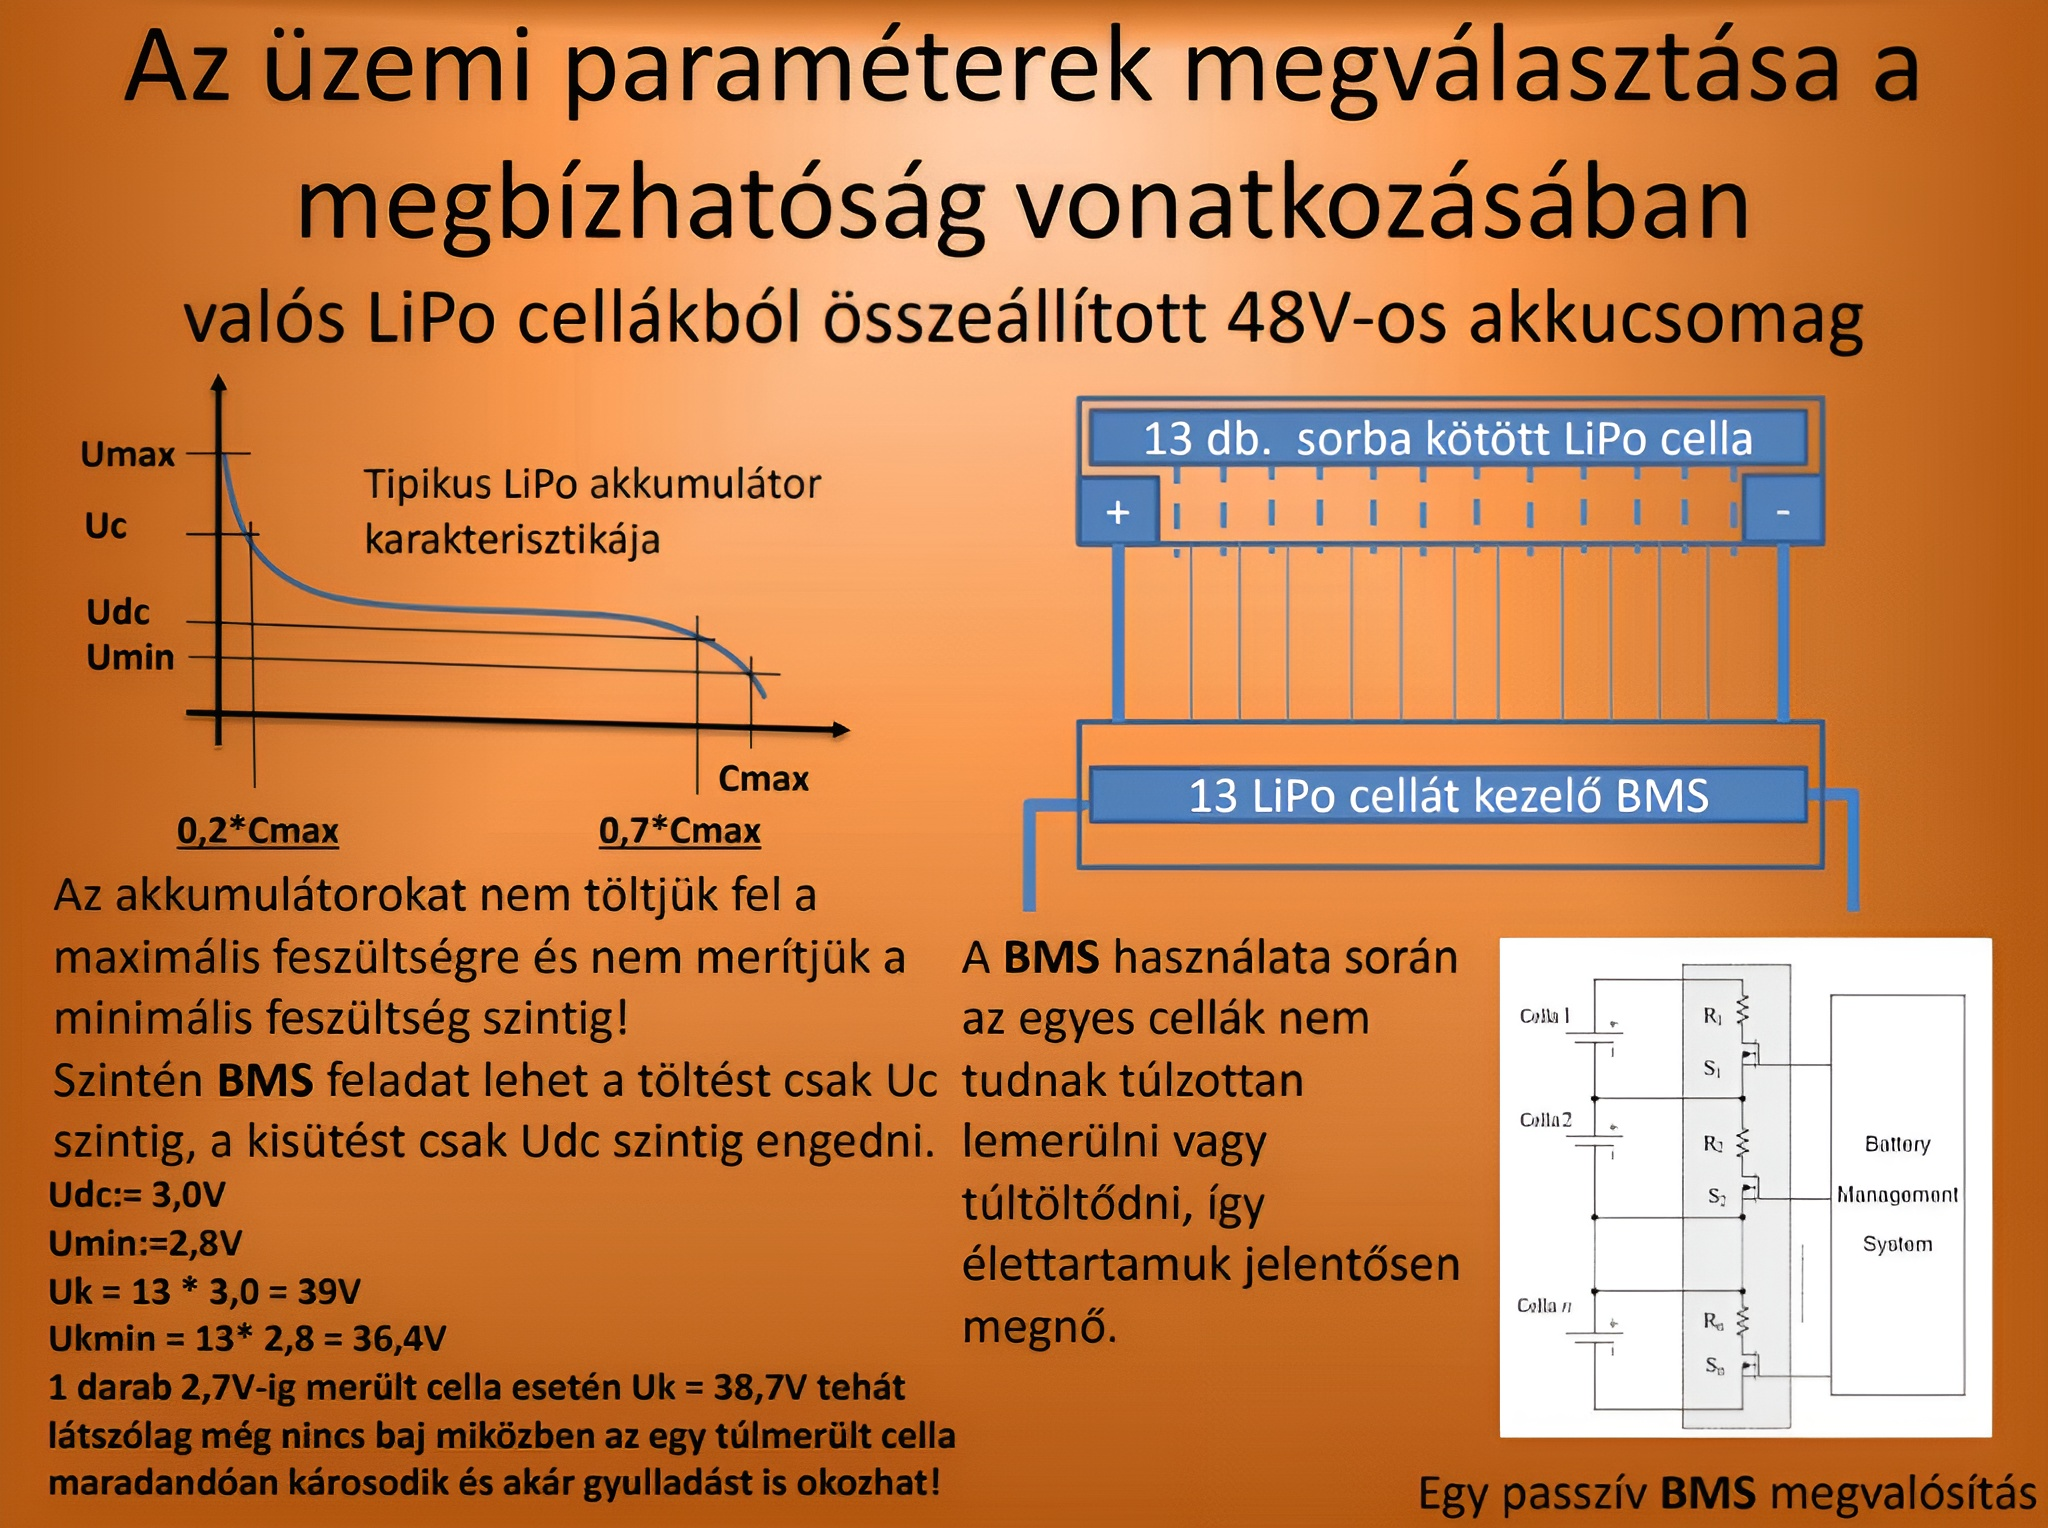
\includegraphics[width=0.7\textwidth]{kep/kep32.png}
    \caption{A BMS jellemzői II.}
    \label{fig:kep32}
\end{figure}

\begin{figure}[H]
    \centering
    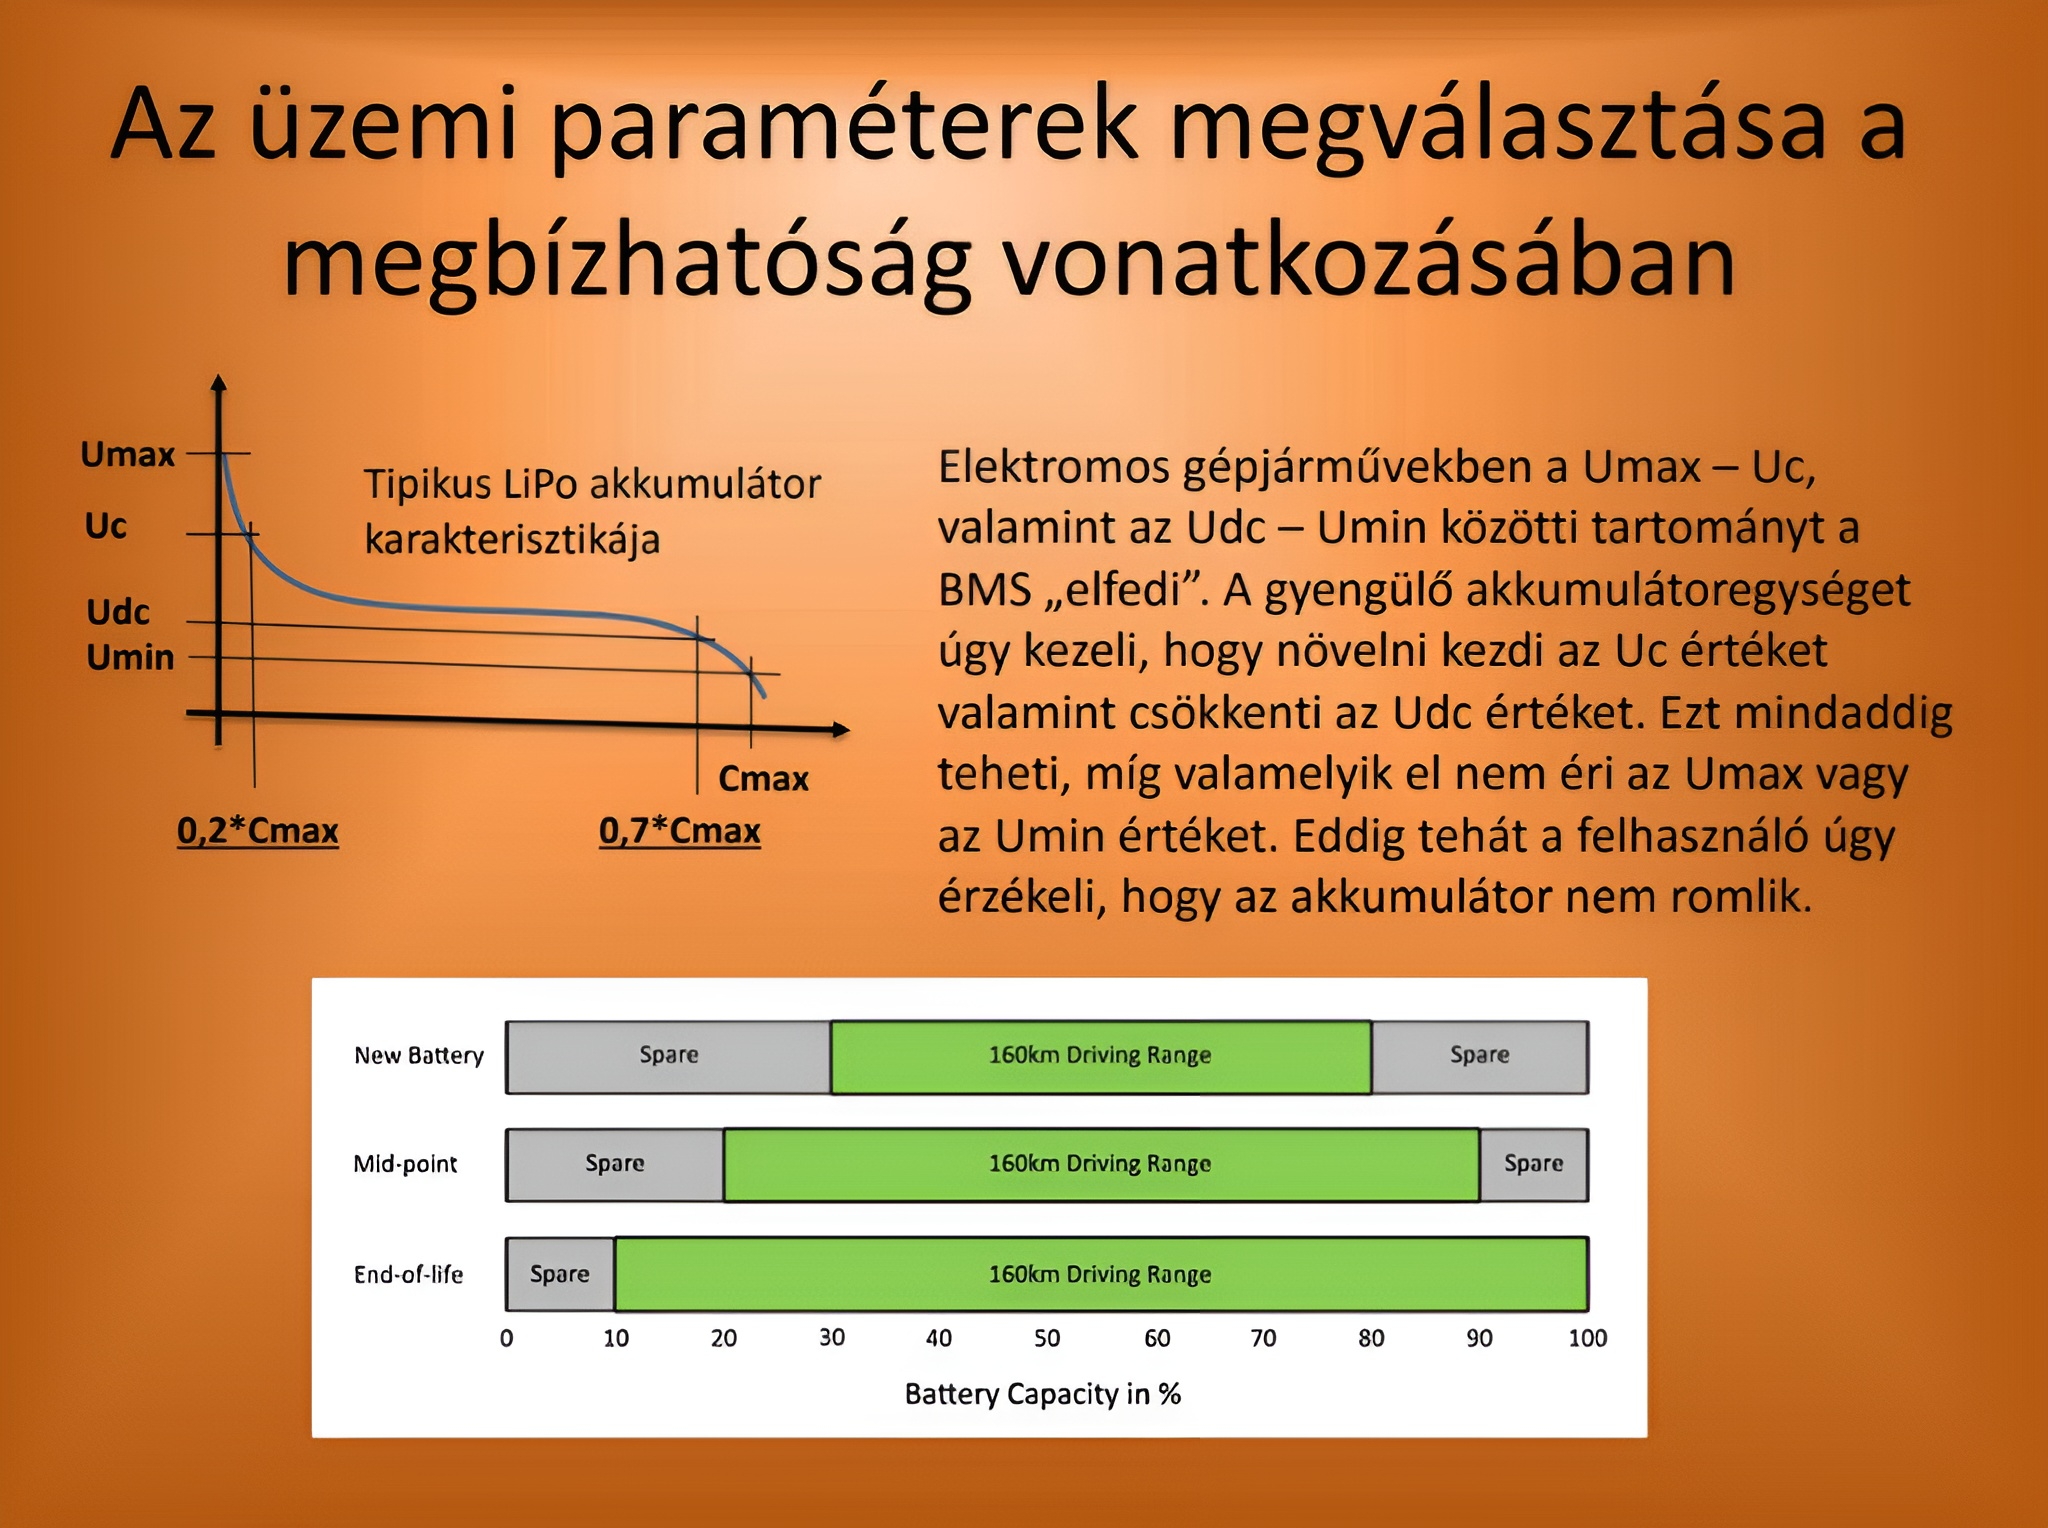
\includegraphics[width=0.7\textwidth]{kep/kep33.png}
    \caption{A BMS jellemzői III.}
    \label{fig:kep33}
\end{figure}

\section{Több forrásból érkező jelek kezelése}

\begin{figure}[H]
    \centering
    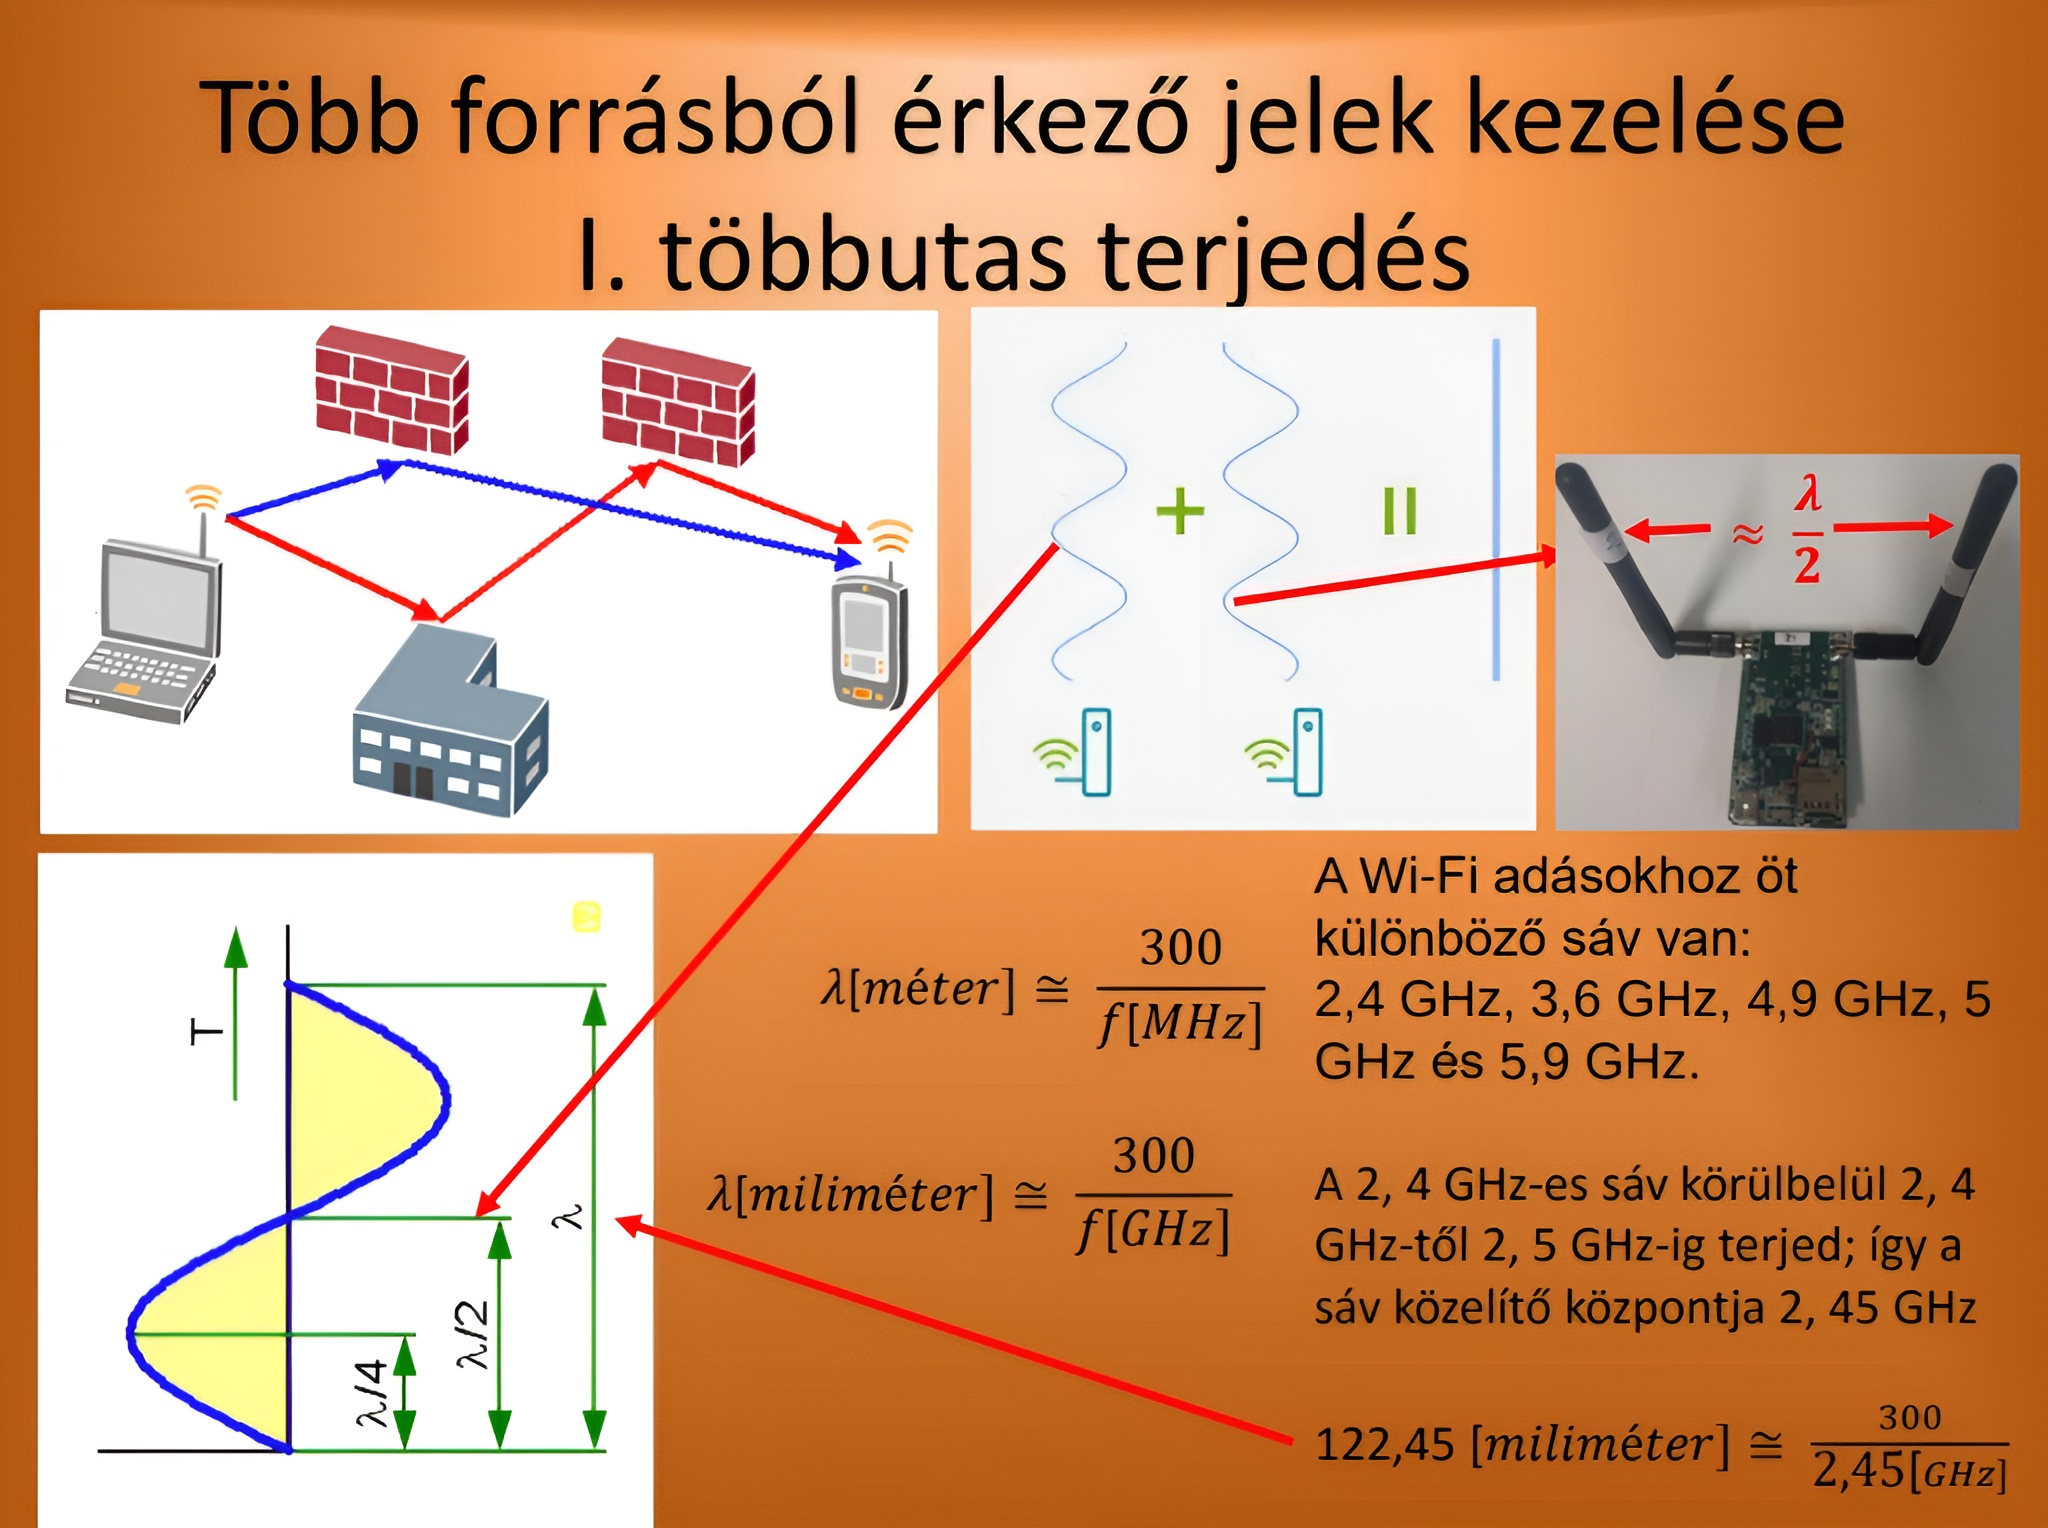
\includegraphics[width=0.7\textwidth]{kep/kep34.png}
    \caption{Több forrásból érkező jelek kezelése I.}
    \label{fig:kep34}
\end{figure}

\begin{figure}[H]
    \centering
    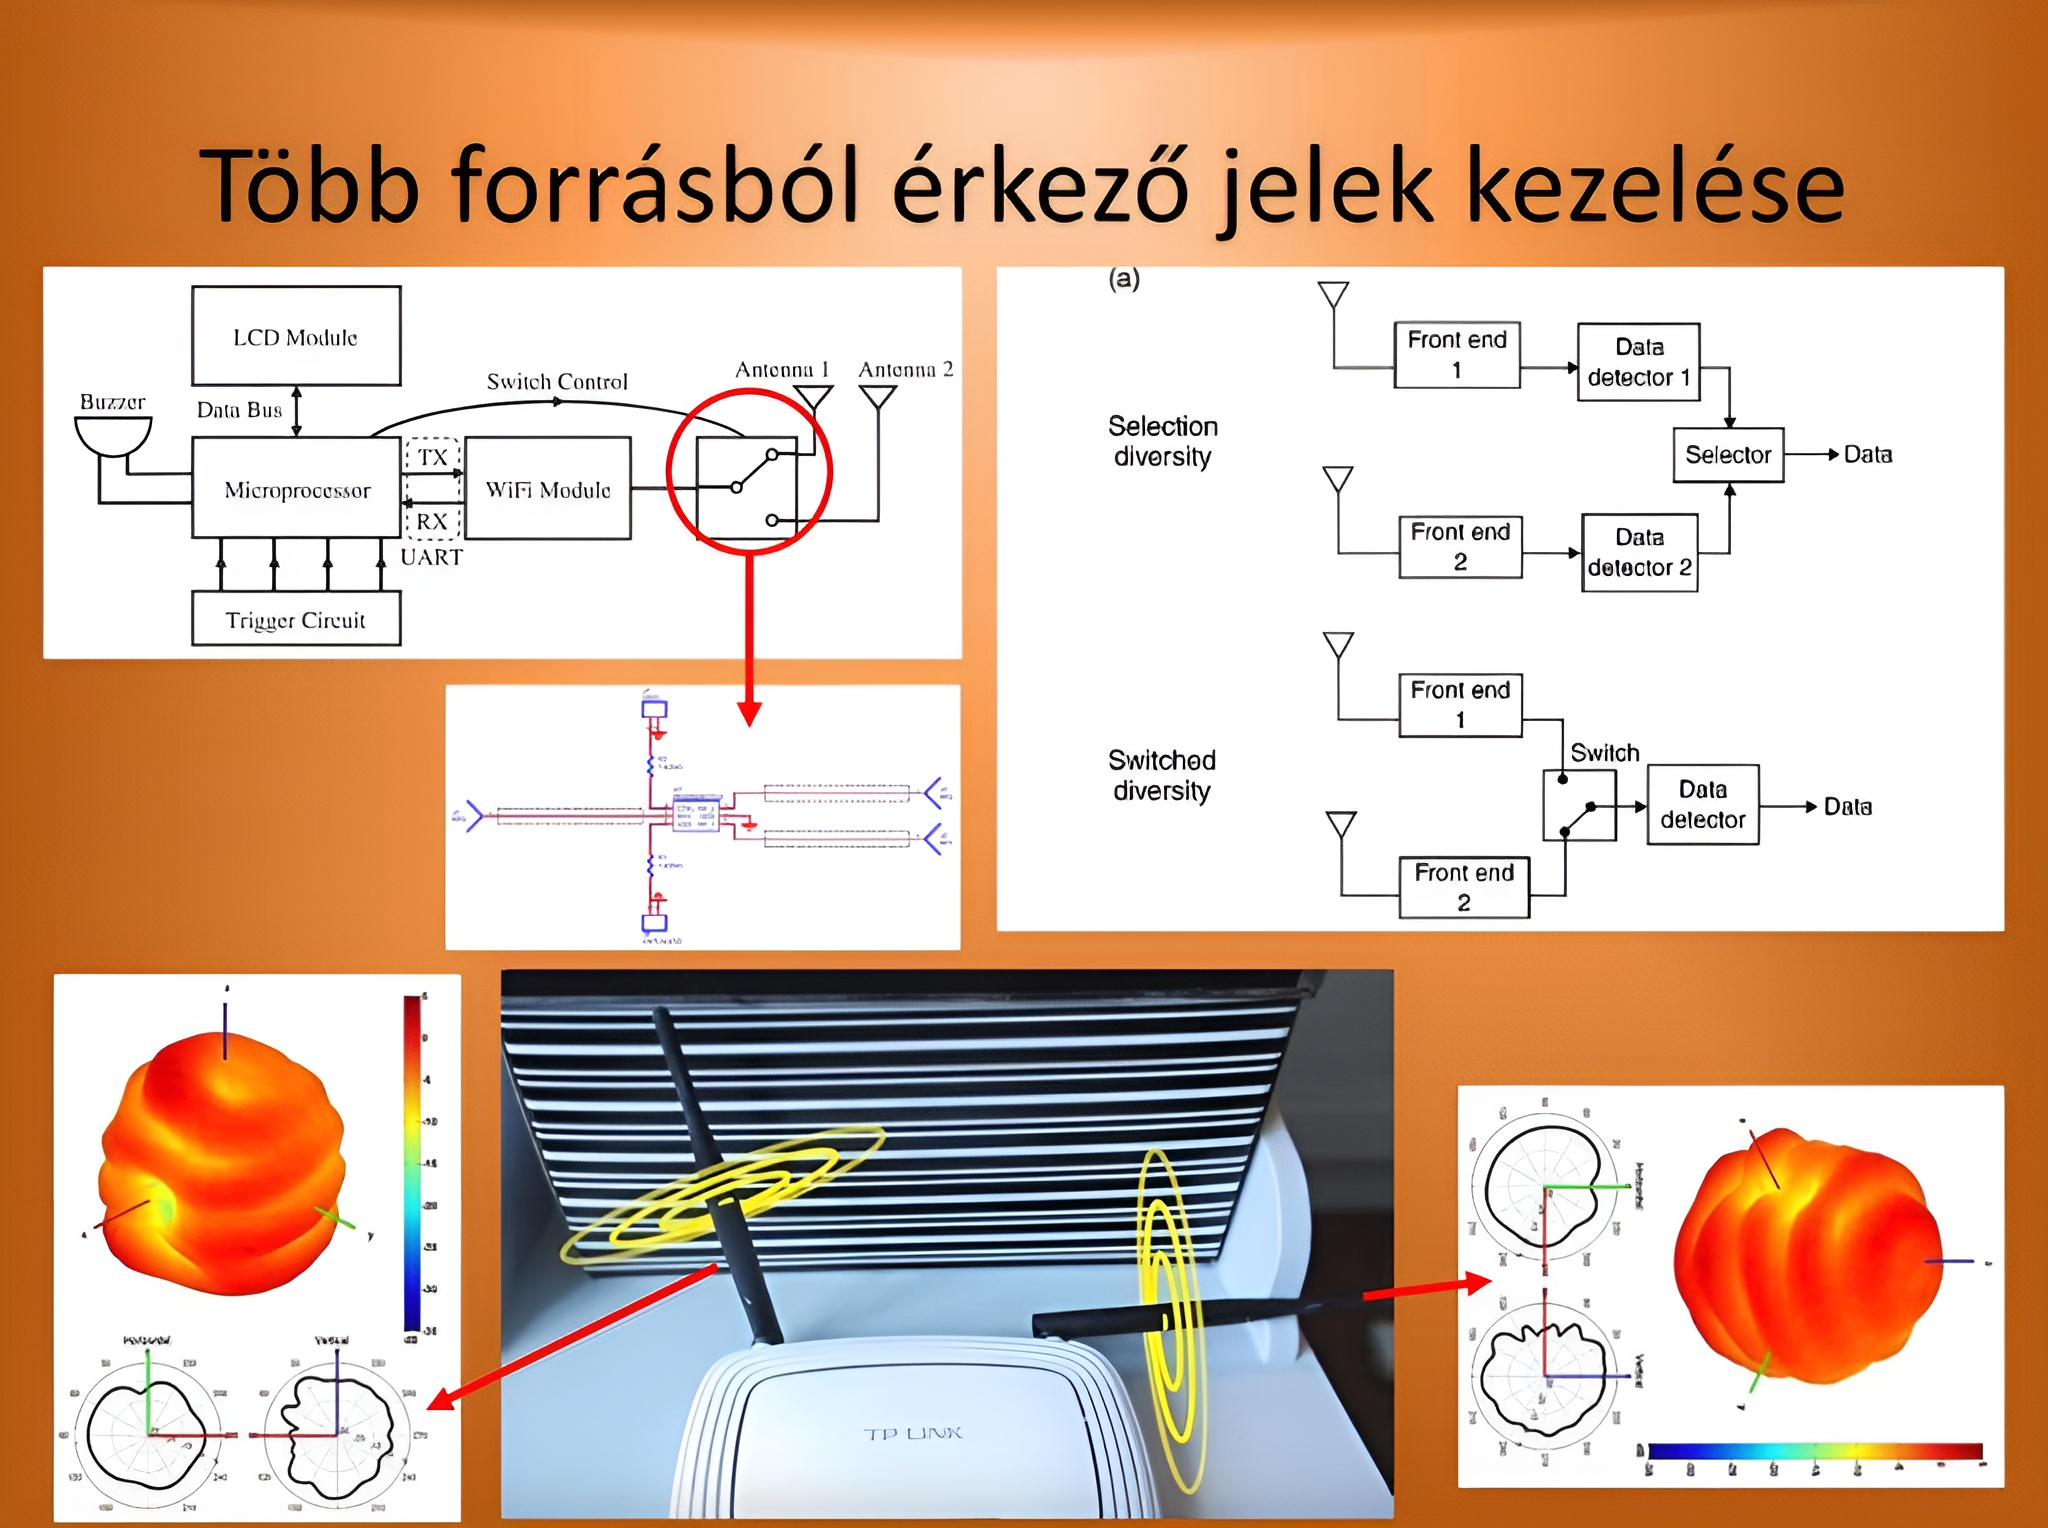
\includegraphics[width=0.7\textwidth]{kep/kep35.png}
    \caption{Több forrásból érkező jelek kezelése II.}
    \label{fig:kep35}
\end{figure}

\begin{itemize}
    \item Több utas terjedés: Több utas terjedés lehet, fázis kioltás történhet, ha éppen olyan helyzetben, pozícióban vannak az eszközök.
    \item Több antennával kezelhető a fáziskioltás problémája.
    \item Számít, hogy az antennák milyen távolságban helyezkednek el egymástól.
    \item Antennák karakterisztikája: irány karakterisztika, merre sugároz vagy honnan tud jól venni jelet.
    \item Több antennás rendszerekkel kezelhető az antenna iránykarakterisztikájának a problémája.
\end{itemize}

\section{Megoldás a több forrásból érkező jelek kezelésére}

\begin{itemize}
    \item Több RC vevő használata, majd szelektorral kiválasztani az egyik működő vevőt és azt a jelet átadni a vezérlőnek.
    \item A vevő interferenciája kezelhető lesz a több vevő használatával, és a csatorna pontos behangolásával.
    \item Ha másik csatorna is üzemel az adott frekvencián, blokkolódhat a jel.
    \item Ilyenkor egy másodlagos frekvenciára kell átállni, az adó sugározhat két frekvencián egyszerre, és hibás jel esetén a vevő átállhat a másodlagos csatornára.
    \item A teljes vezérlő jel kiesése kezelhető, ha a kapcsolat megszűnése esetén az eszköz átállautonóm működésre.
    \item Például a modellrepülő a távirányító vezérléséről átáll egy beépített robotpilótára. Programhiba, vagy más meghibásodás esetén átállhat egy másodlagos robotpilóta vezérlésére.
    \item Amennyiben másik frekvencián a robotpilótával van működő kapcsolat, adható számára parancs vagy vezérlés, hogy melyik irányba, vagy hogyan repüljön, anélkül hogy a felhasználónak kéne kormányoznia a távirányítón.
\end{itemize}

\begin{figure}[H]
    \centering
    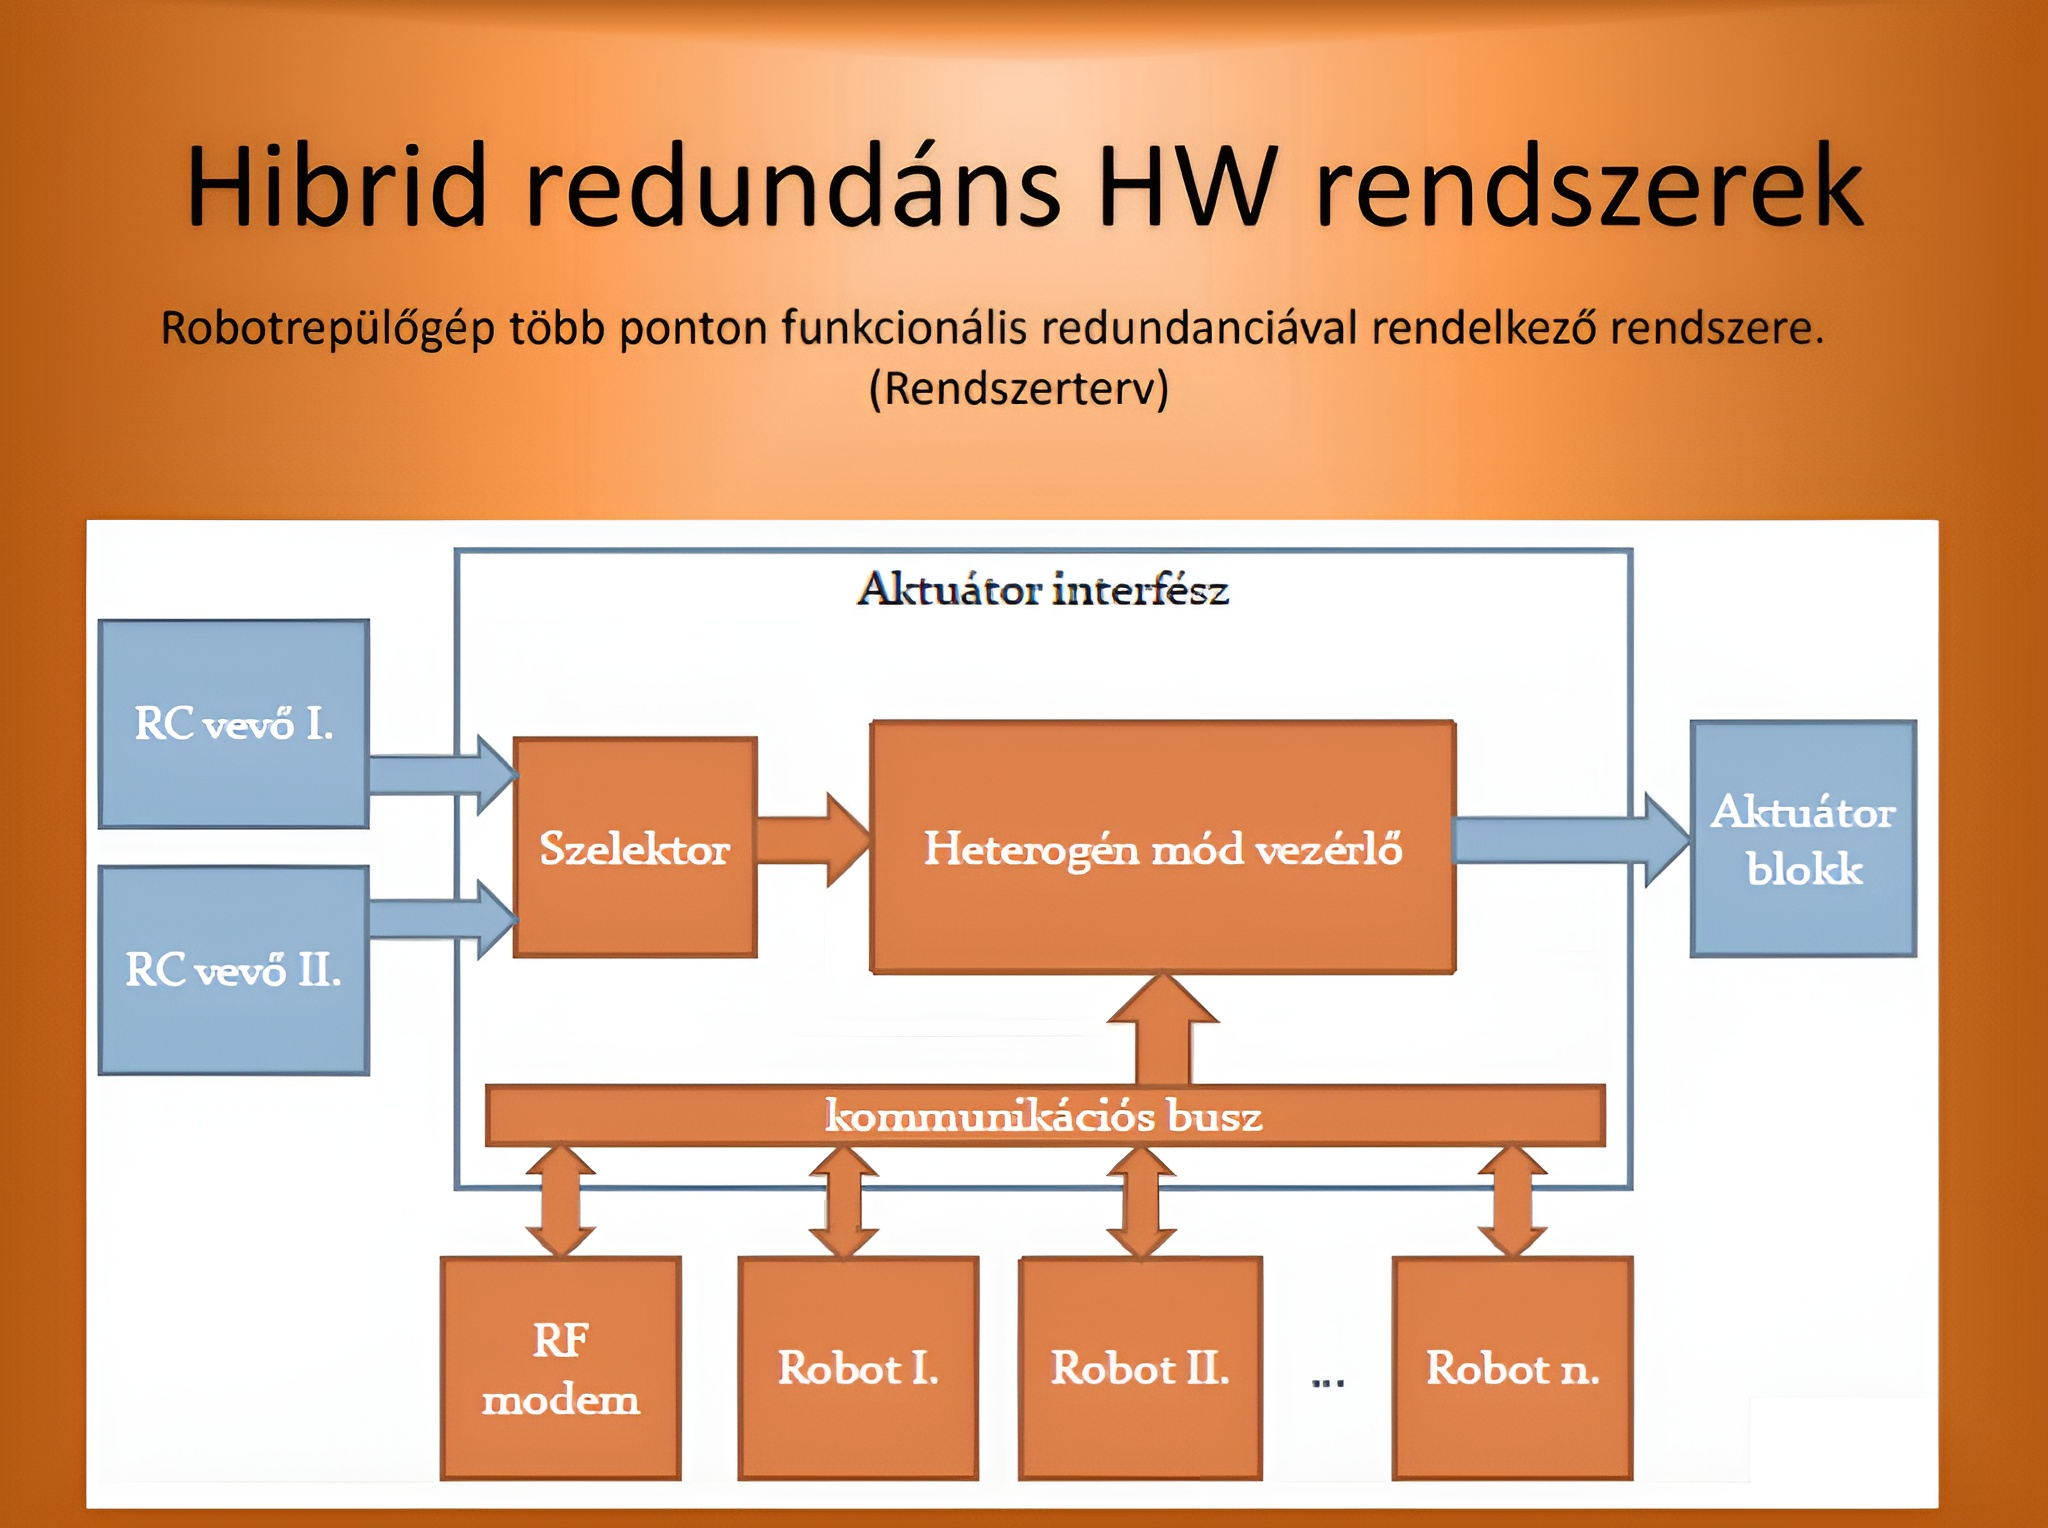
\includegraphics[width=0.7\textwidth]{kep/kep36.png}
    \caption{Több forrásból érkező jelek kezelése III.}
    \label{fig:kep36}
\end{figure}

\begin{figure}[H]
    \centering
    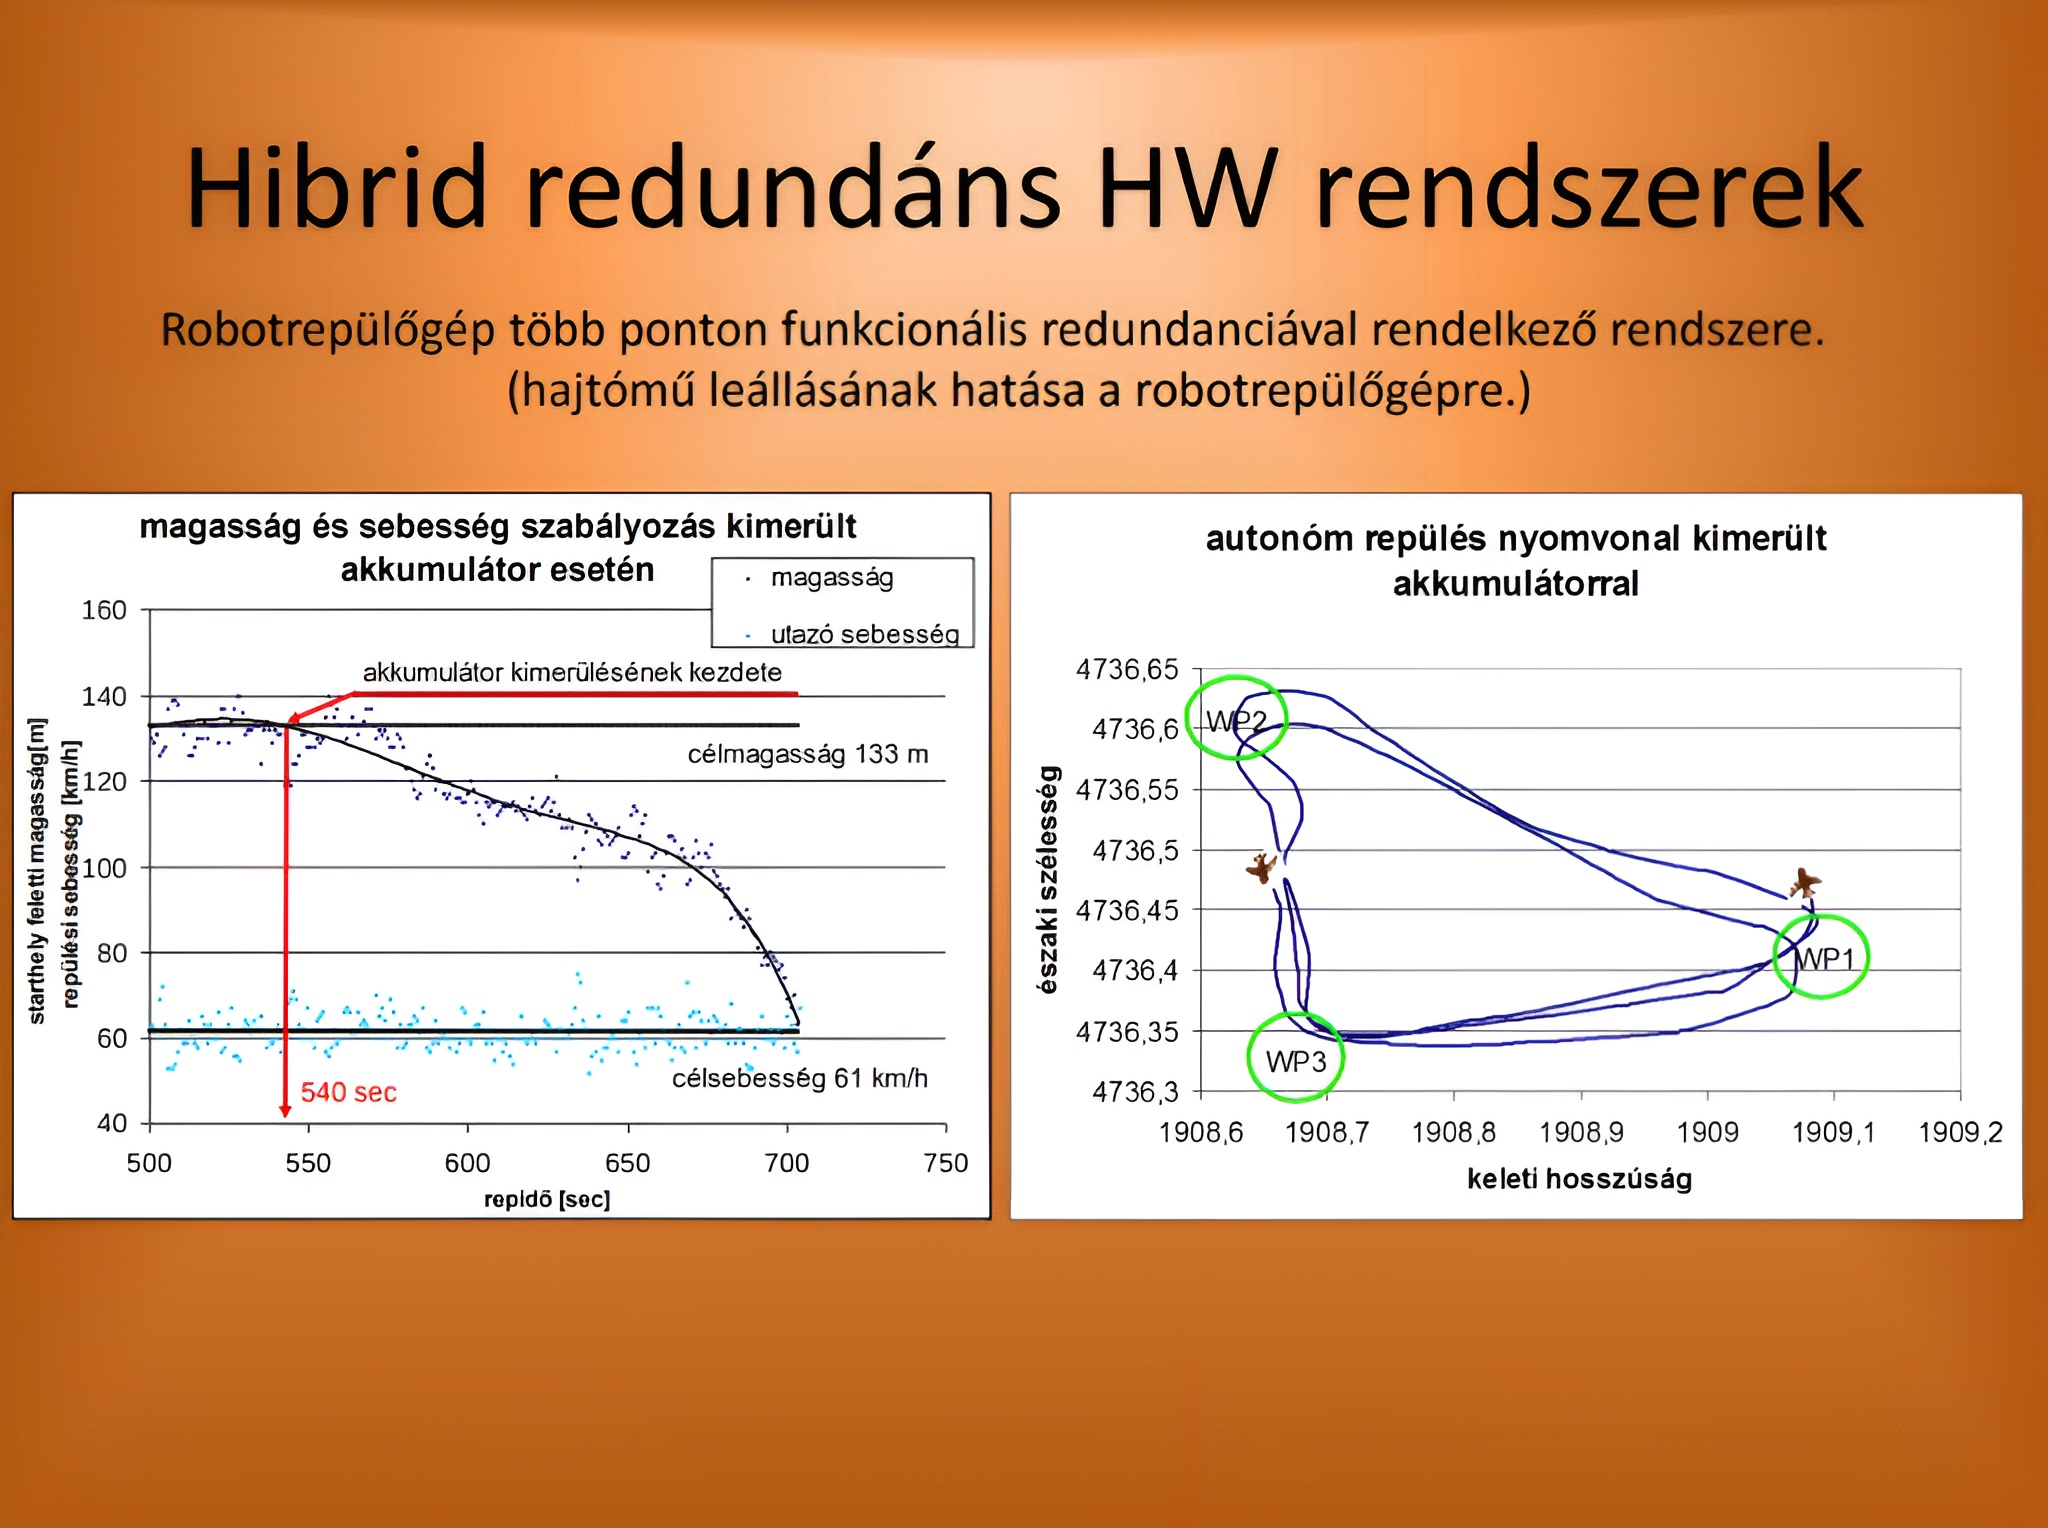
\includegraphics[width=0.7\textwidth]{kep/kep37.png}
    \caption{Több forrásból érkező jelek kezelése IV.}
    \label{fig:kep37}
\end{figure}

\section{FPGA vezérlő alkalmazása}

\begin{itemize}
    \item Egy-egy hardveres út meghibásodása esetén van rá lehetőség, hogy azok kihagyásával programozzuk újra a chipet, így még használható marad csökkentett tudással.
    \item Akár futásidőben újrakonfigurálható hardveregységek is megvalósíthatók.
    \item Léteznek biztosíték jellegű vezetékek, tehát kiégethetők. Ez a típusú chip csak egyszer programozható.
    \item Analóg rendszerekkel is megvalósítható programozható áramkör.
\end{itemize}

\subsection{Szimulációs többségi redundancia}

\begin{itemize}
    \item Több panelt, pl. 3db Arduinot bekötünk
    \item Tincercad szimuláció
    \item Csak szinkron módban működik
\end{itemize}

\subsection{Jelminőségen alapuló redundancia}

\begin{itemize}
    \item Pl. 2db Arduino bekötése
    \item Egy szavazó áramkör alkalmazása
\end{itemize}

\begin{figure}[H]
    \centering
    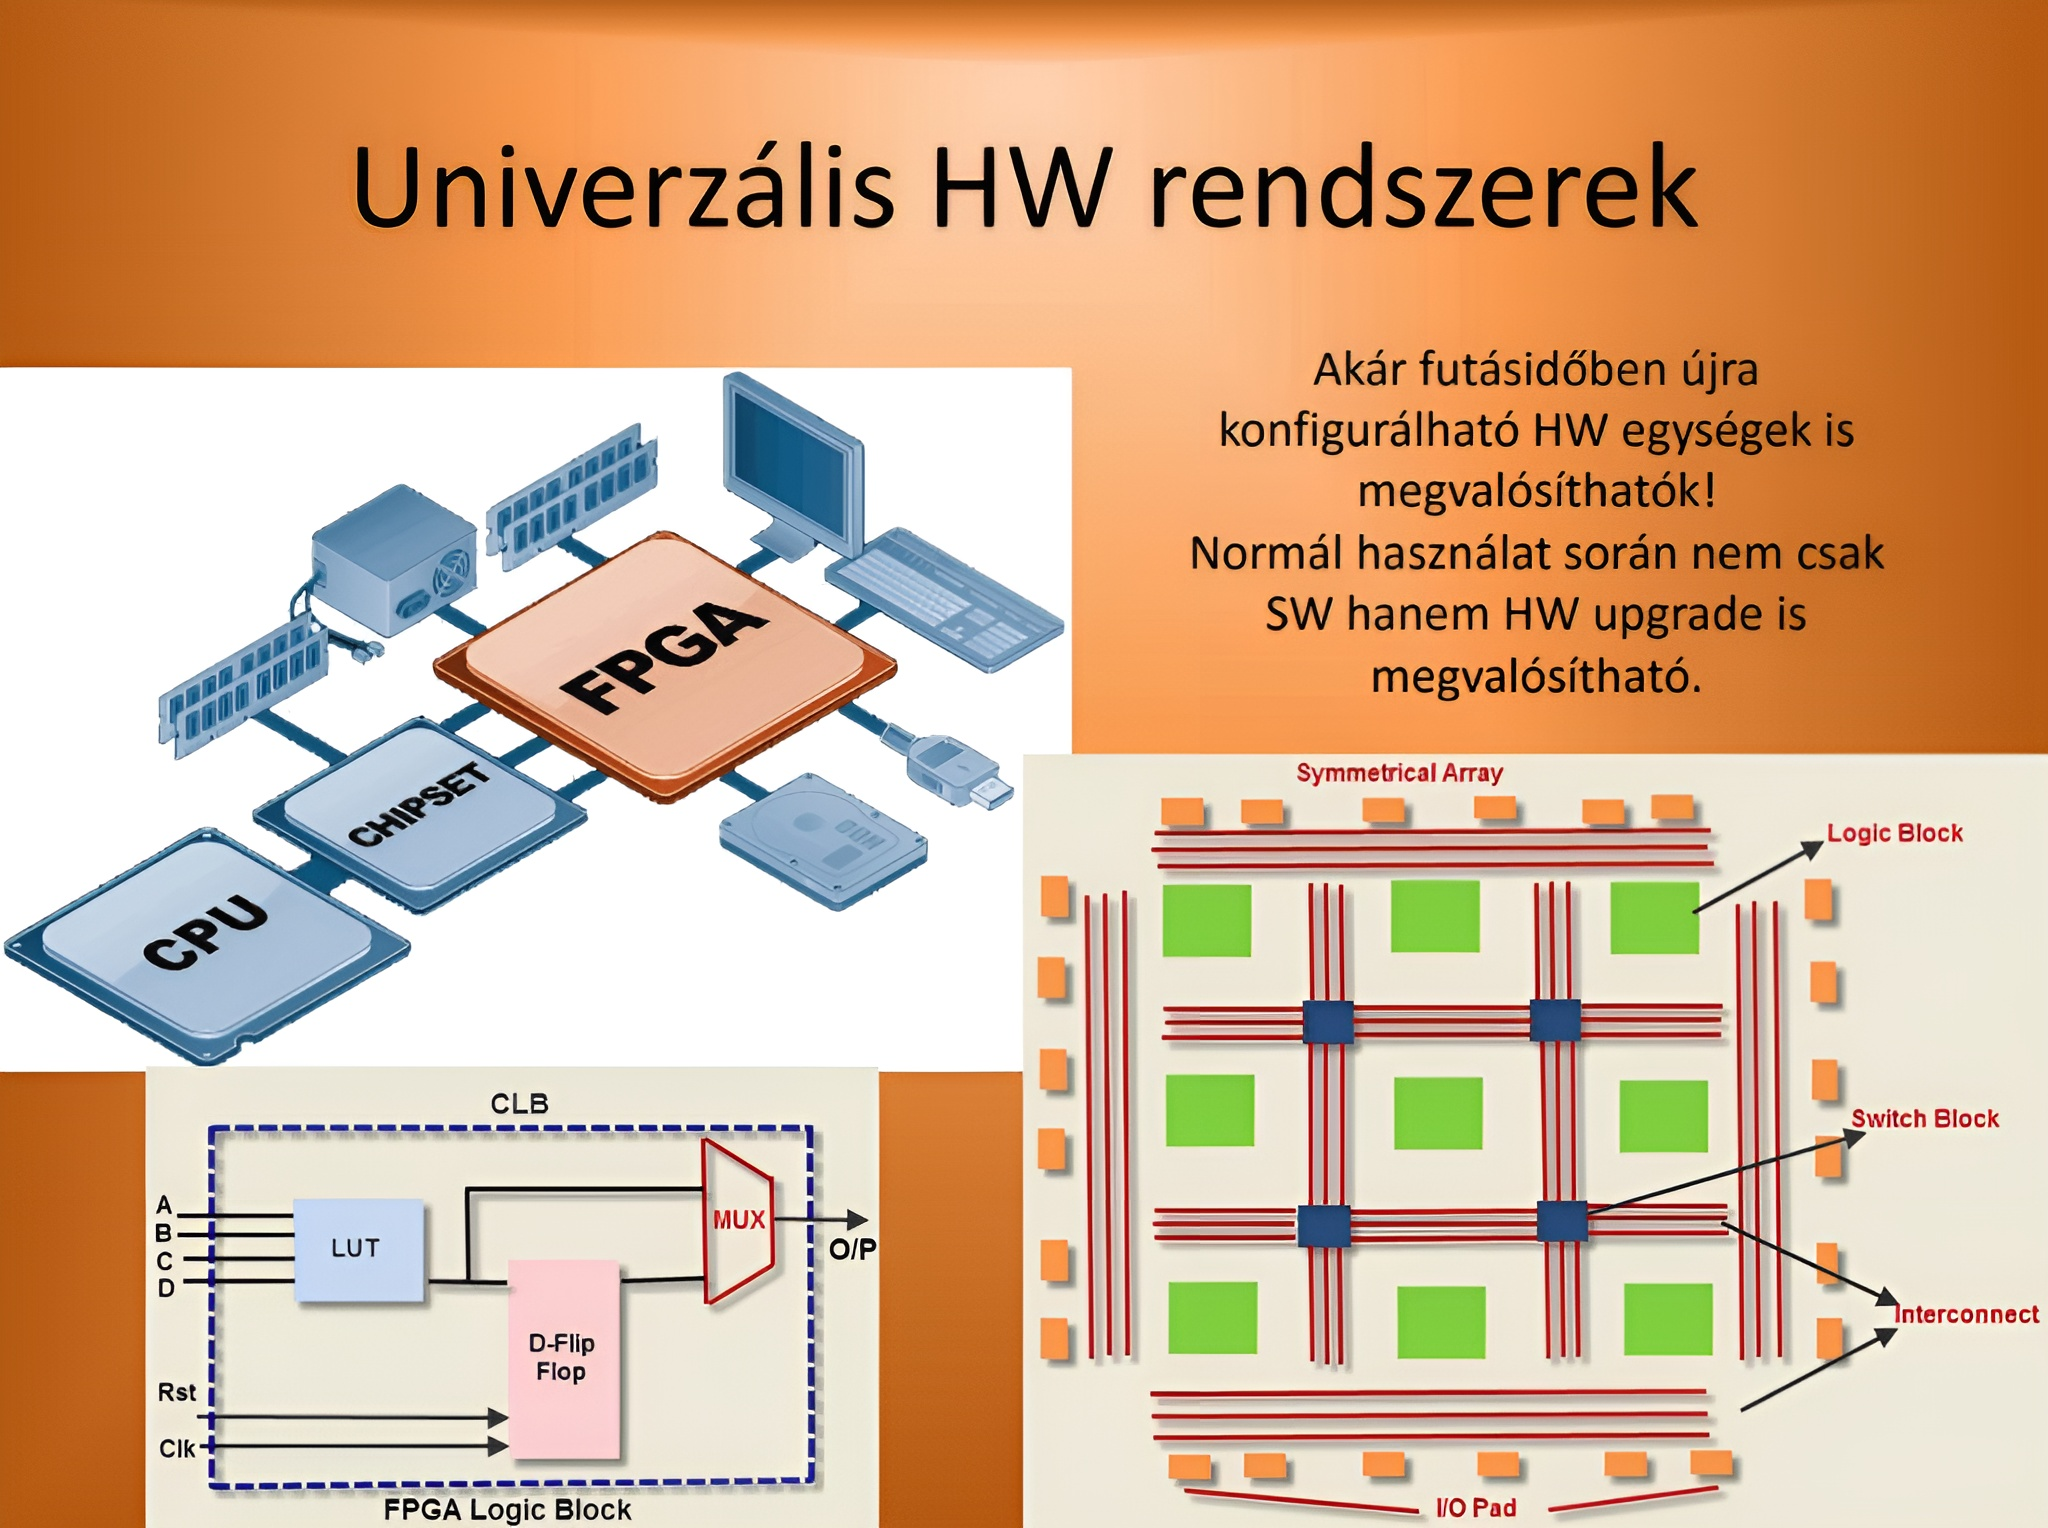
\includegraphics[width=0.7\textwidth]{kep/kep38.png}
    \caption{FPGA vezérlő I.}
    \label{fig:kep38}
\end{figure}

\begin{figure}[H]
    \centering
    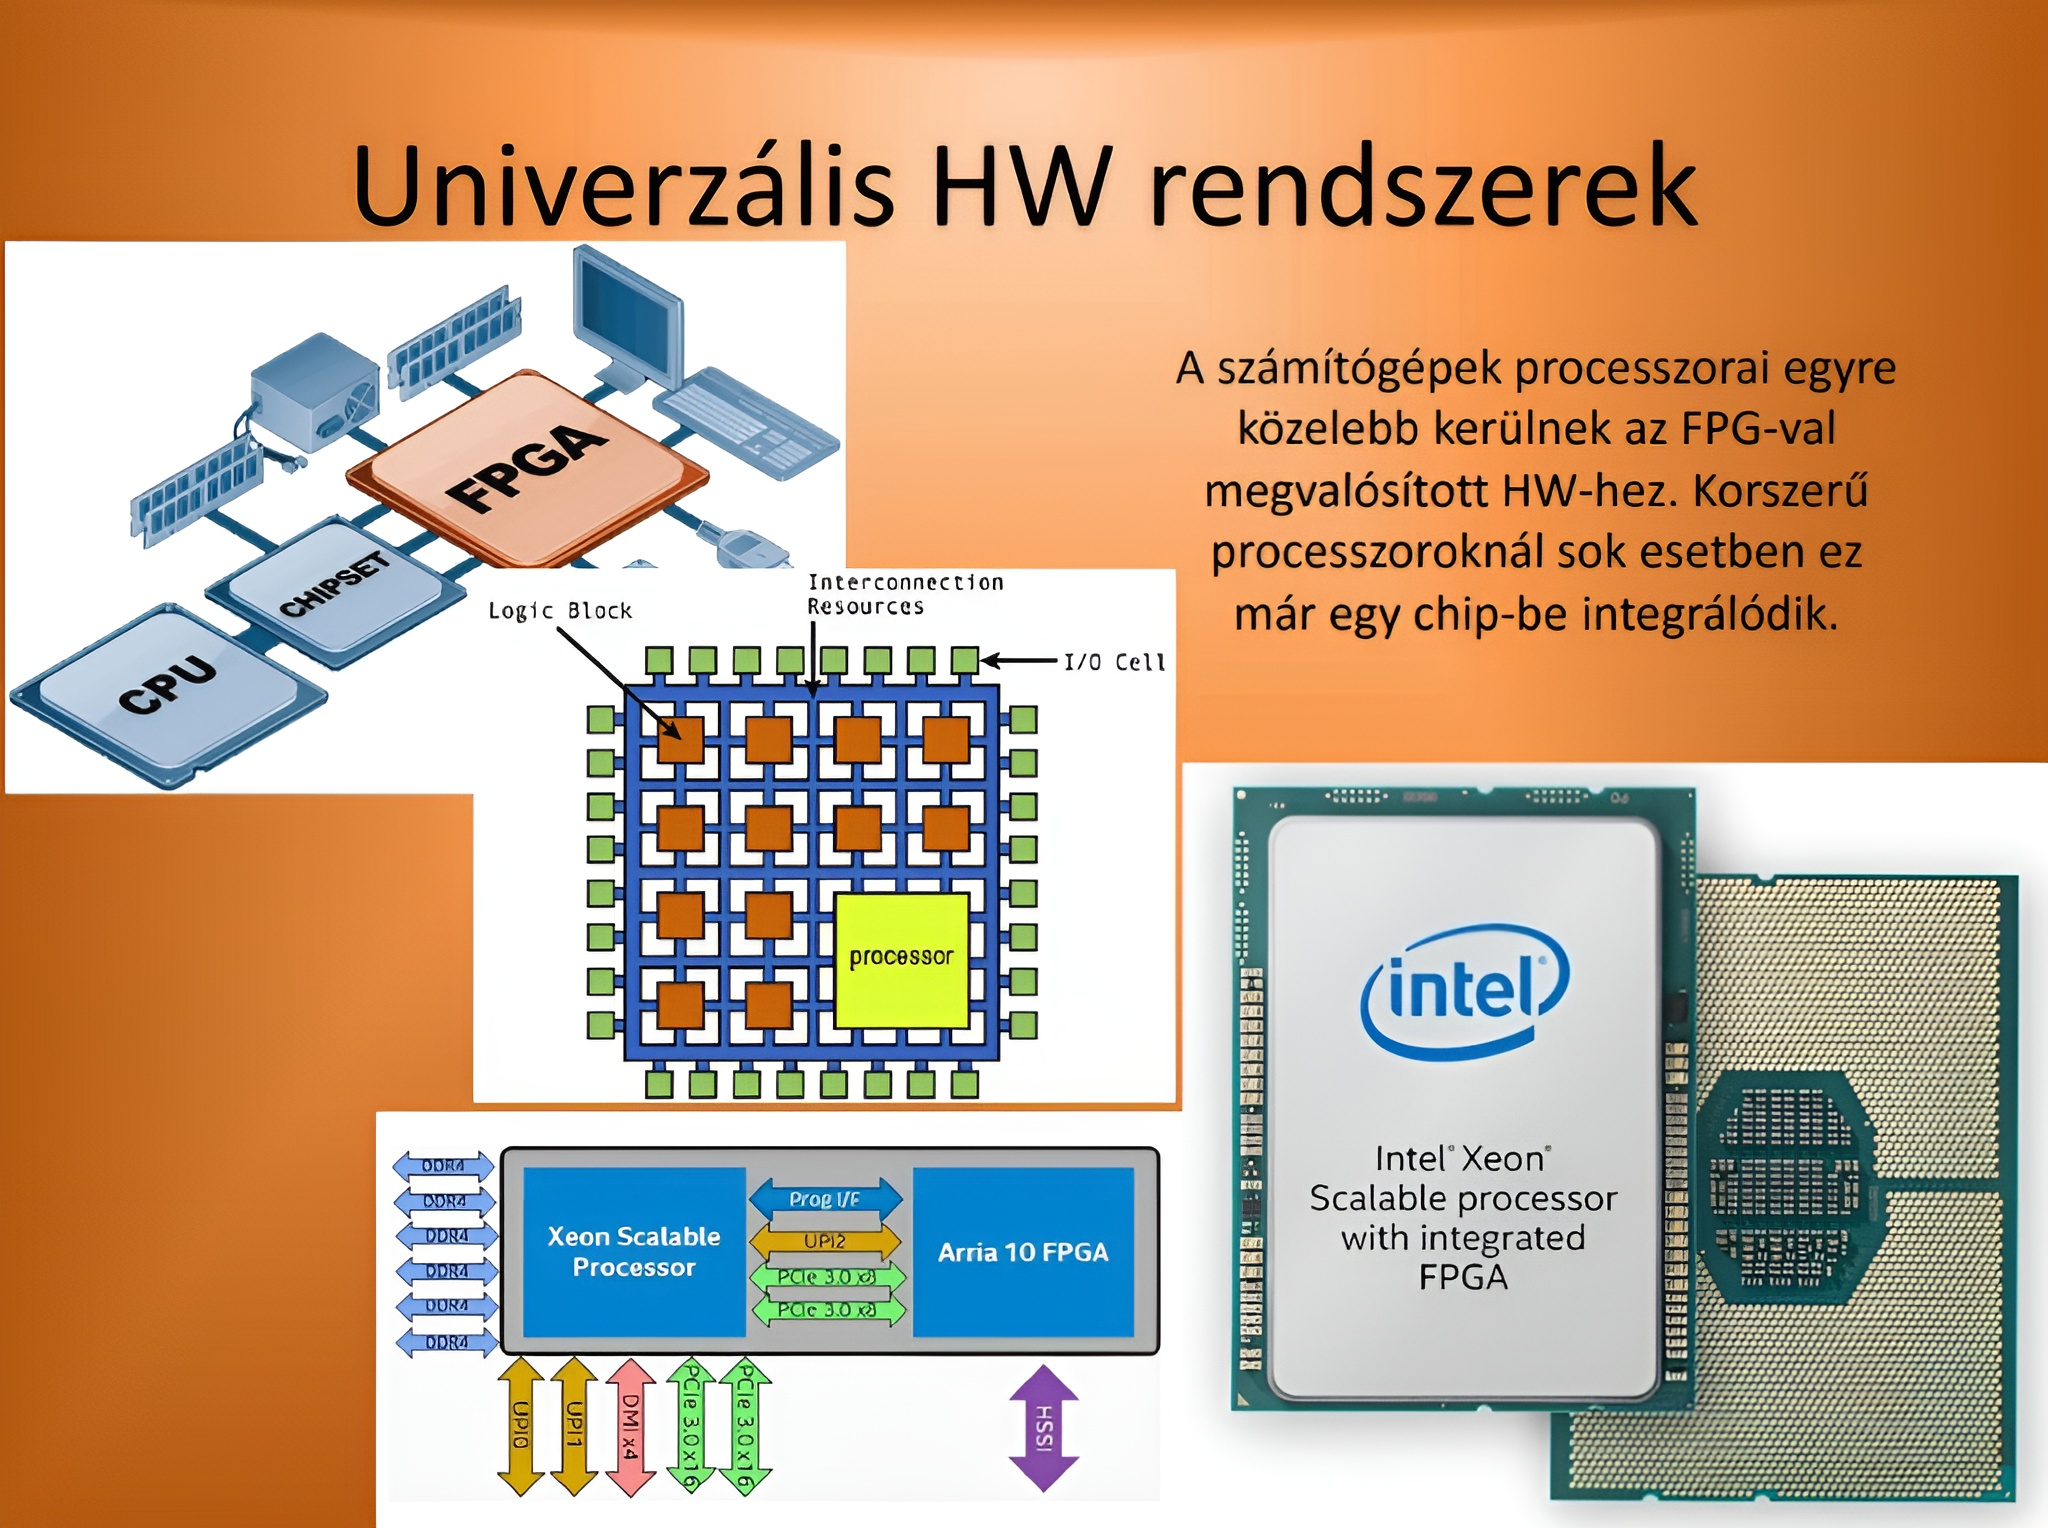
\includegraphics[width=0.7\textwidth]{kep/kep39.png}
    \caption{FPGA vezérlő II.}
    \label{fig:kep39}
\end{figure}

\begin{figure}[H]
    \centering
    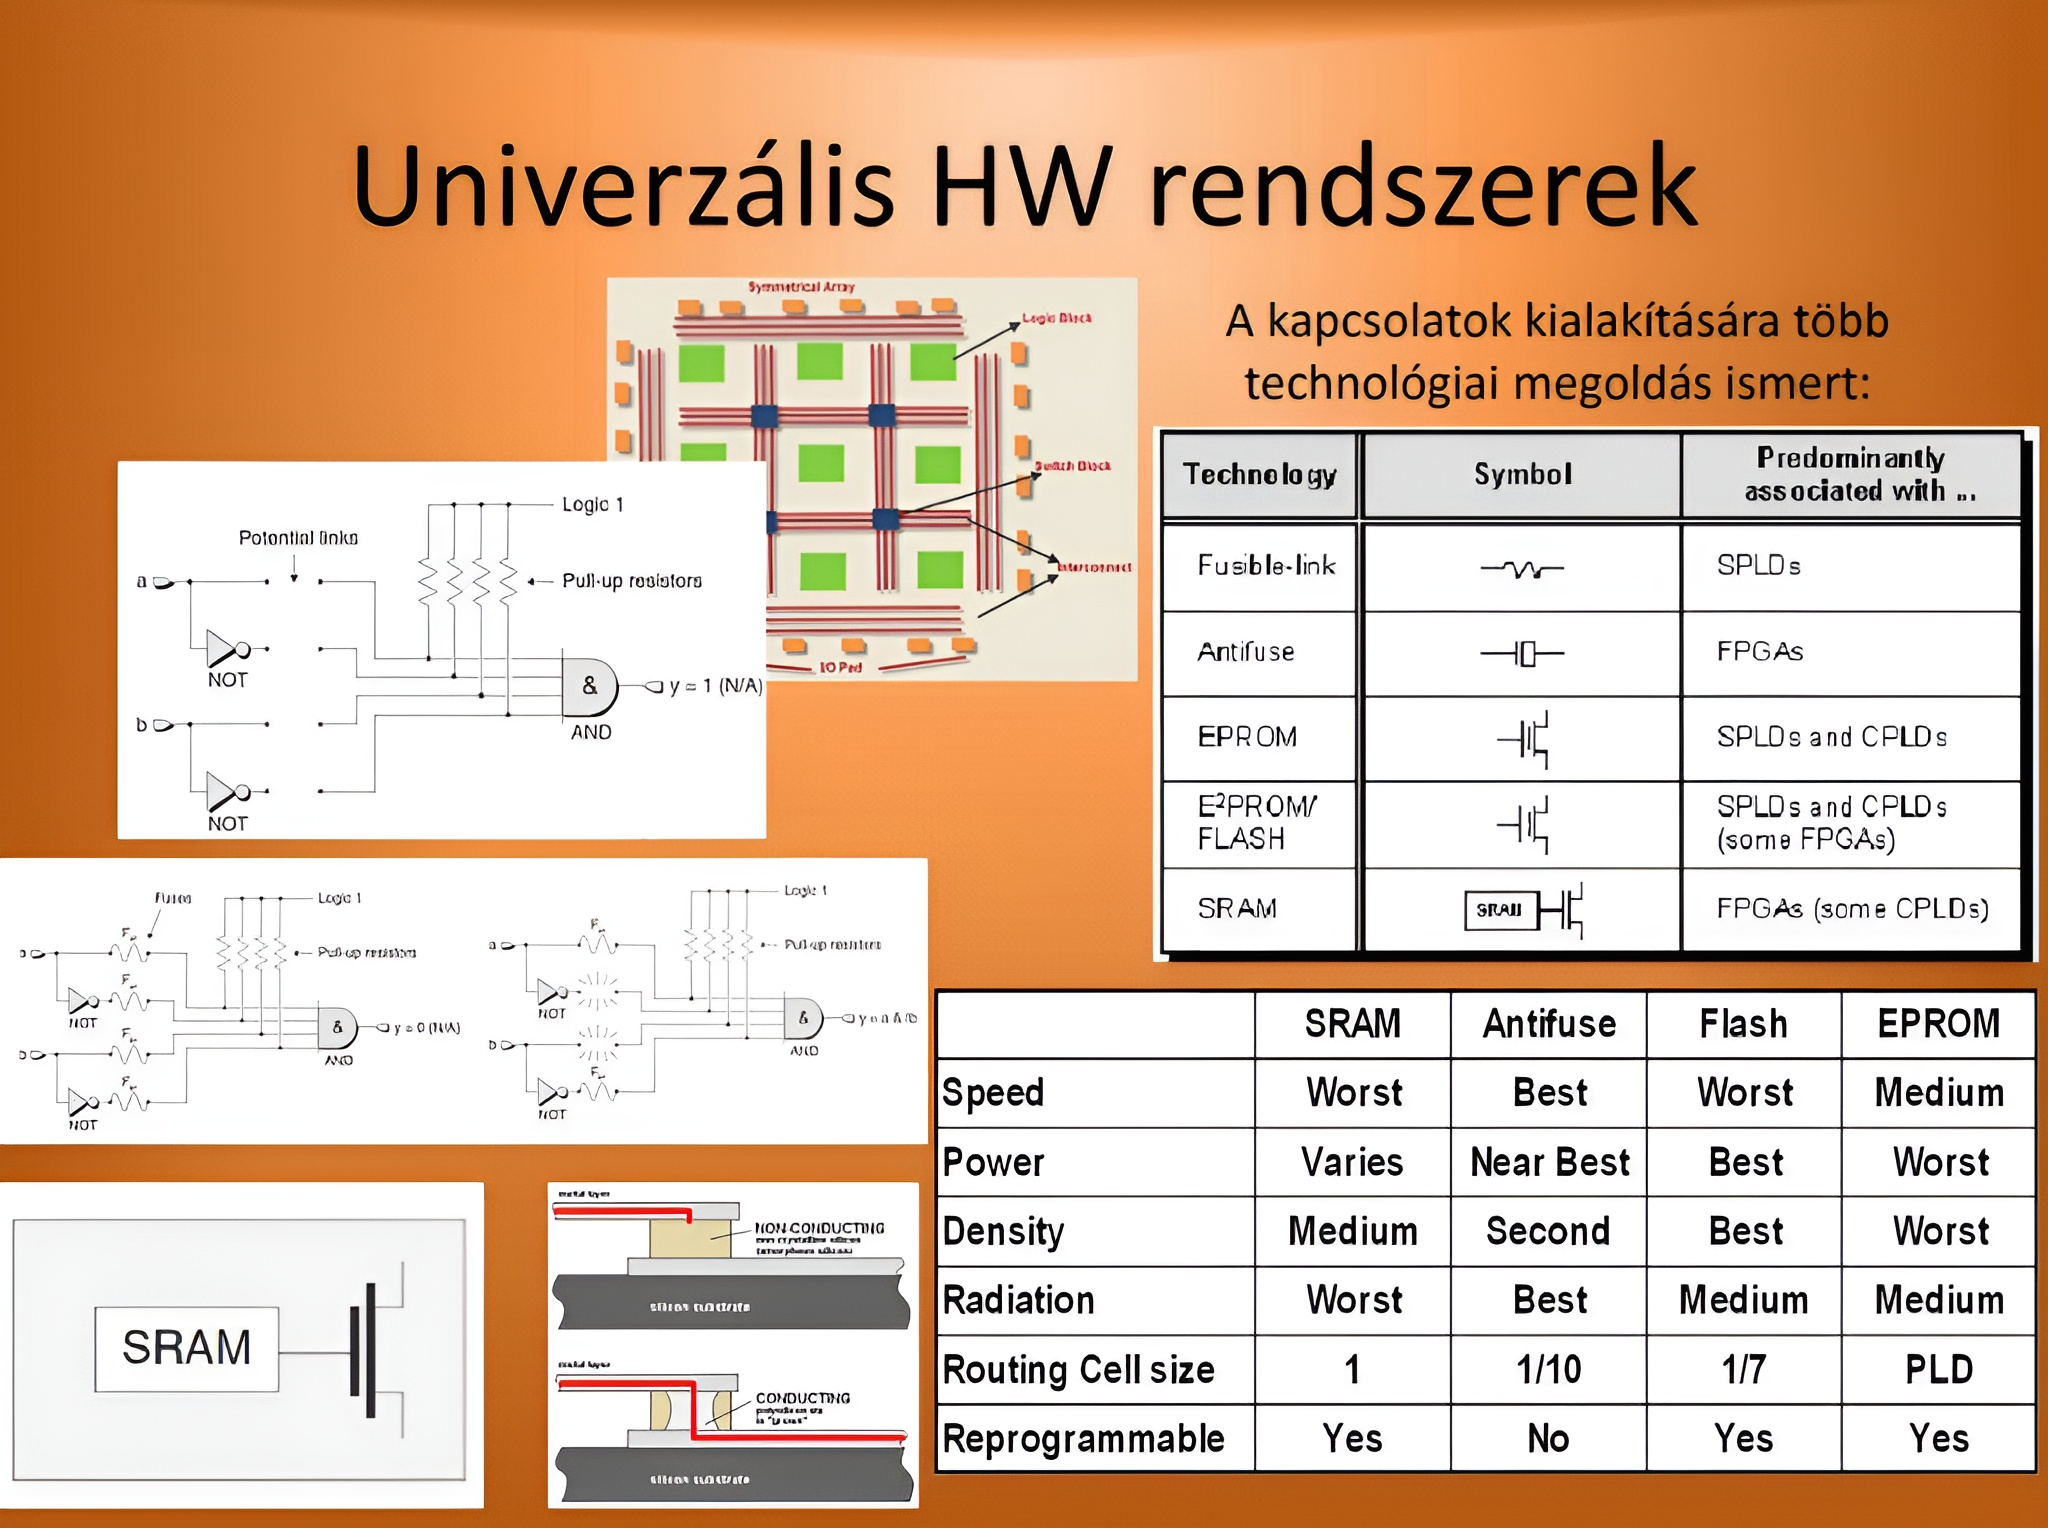
\includegraphics[width=0.7\textwidth]{kep/kep40.png}
    \caption{FPGA vezérlő III.}
    \label{fig:kep40}
\end{figure}

\end{document}
